%%%%%%%%%%%%%%%%%%%%%%%%%%%%%%%%%%%%%%%%%
% Journal Article
% LaTeX Template
% Version 1.4 (15/5/16)
%
% This template has been downloaded from:
% http://www.LaTeXTemplates.com
%
% Original author:
% Frits Wenneker (http://www.howtotex.com) with extensive modifications by
% Vel (vel@LaTeXTemplates.com)
%
% License:
% CC BY-NC-SA 3.0 (http://creativecommons.org/licenses/by-nc-sa/3.0/)
%
%%%%%%%%%%%%%%%%%%%%%%%%%%%%%%%%%%%%%%%%%

%----------------------------------------------------------------------------------------
%	PACKAGES AND OTHER DOCUMENT CONFIGURATIONS
%----------------------------------------------------------------------------------------

\documentclass[twoside,onecolumn]{article}

\usepackage[sc]{mathpazo} % Use the Palatino font
\usepackage[T1]{fontenc} % Use 8-bit encoding that has 256 glyphs
\linespread{1.05} % Line spacing - Palatino needs more space between lines
\usepackage{microtype} % Slightly tweak font spacing for aesthetics

\usepackage[english]{babel} % Language hyphenation and typographical rules

\usepackage[hmarginratio=1:1,top=32mm,columnsep=20pt]{geometry} % Document margins
\usepackage[hang, small,labelfont=bf,up,textfont=it,up]{caption} % Custom captions under/above floats in tables or figures
\usepackage{booktabs} % Horizontal rules in tables

\usepackage{lettrine} % The lettrine is the first enlarged letter at the beginning of the text

\usepackage{enumitem} % Customized lists
\setlist[itemize]{noitemsep} % Make itemize lists more compact

\usepackage{abstract} % Allows abstract customization
\renewcommand{\abstractnamefont}{\normalfont\bfseries} % Set the "Abstract" text to bold
\renewcommand{\abstracttextfont}{\normalfont\small\itshape} % Set the abstract itself to small italic text

\usepackage{titlesec} % Allows customization of titles
\renewcommand\thesection{\Roman{section}} % Roman numerals for the sections
\renewcommand\thesubsection{\roman{subsection}} % roman numerals for subsections
\titleformat{\section}[block]{\large\scshape\centering}{\thesection.}{1em}{} % Change the look of the section titles
\titleformat{\subsection}[block]{\large}{\thesubsection.}{1em}{} % Change the look of the section titles

\usepackage{fancyhdr} % Headers and footers
\usepackage{lastpage}
\pagestyle{fancy} % All pages have headers and footers
\fancyhead{} % Blank out the default header
\fancyfoot{} % Blank out the default footer
\fancyhead[C]{$\bullet$ Tone and genes: new data and methods $\bullet$} % Custom header text
\fancyfoot[RO,LE]{\thepage/\pageref{LastPage}} % Custom footer text

\usepackage{titling} % Customizing the title section

\usepackage{hyperref} % For hyperlinks in the PDF
\hypersetup{
	colorlinks=true,
	linkcolor=blue,
	filecolor=blue,
	urlcolor=blue,
	citecolor=blue,
	bookmarks=true,
	hyperindex=true,
}
\urlstyle{same}

\usepackage{enumitem} % lists

\usepackage{graphicx} % figures
\usepackage[outdir=./]{epstopdf} % EPS figures
\usepackage{tikz} % Tikz figures
\usepackage{subcaption} % subfigures

\usepackage{tabularx} % tables
\usepackage{multirow}
\usepackage{makecell}

\usepackage{amsmath} % math

\usepackage{doi}
\usepackage{natbib} % References
\bibliographystyle{plainnat} % APA


%----------------------------------------------------------------------------------------
%	TITLE SECTION
%----------------------------------------------------------------------------------------

\setlength{\droptitle}{-4\baselineskip} % Move the title up

\pretitle{\begin{center}\Huge\bfseries} % Article title formatting
\posttitle{\end{center}} % Article title closing formatting
\title{Tone and genes: new data and methods support the negative effect of the ``derived'' allele of \textit{ASPM} on tone, but not of \textit{Microcephalin}} % Article title
\author{%
\textsc{Dan Dediu} \\[1ex] % Your name
\normalsize Laboratoire Dynamique Du Language (DDL) UMR5596,\\
\normalsize Université Lumière Lyon 2, Lyon, France \\ % Your institution
\normalsize \href{mailto:dan.dediu@univ-lyon2.fr}{dan.dediu@univ-lyon2.fr} % Your email address
%\and % Uncomment if 2 authors are required, duplicate these 4 lines if more
%\textsc{Jane Smith}\thanks{Corresponding author} \\[1ex] % Second author's name
%\normalsize University of Utah \\ % Second author's institution
%\normalsize \href{mailto:jane@smith.com}{jane@smith.com} % Second author's email address
}
\date{\today} % Leave empty to omit a date
\renewcommand{\maketitlehookd}{%
\begin{abstract}
\noindent While it is generally accepted that language and speech have genetic foundations, and that the widespread inter-individual variation observed in many of their aspects is partly driven by variation in genes, it is much less clear if differences between languages may aso be partly rooted in our genes.
One such proposal is that the frequencies of the so-called ``derived'' alleles of two genes involved in brain growth and development, \textit{ASPM} and \textit{Microcephalin}, in a population are related to the probability that the population speaks a tone language or not.
The study used a cross-linguistic statistical approach, showing that these associations are ``special'' when considered to many other possible relationships between human geentic variants and linguistic features.
Recently, experimental evidence became available that strongly supports the proposal that the ``derived'' allele of \textit{ASPM} influences tone perception and/or processing within individuals, but that failed to find any effect of \textit{Microcephalin}.
Motivated by these experimental findings, I conduct here a cross-linguistic statistical test of these hypotheses, using a larger and updated dataset of 175 samples from 129 unique (meta)populations, and a battery of methods including mixed-effects regressionm, mediation and path analysis, decision trees and random forests, using permutations and restricted samping to control for the confounding effects of genealogy (language familis) and contact (macroareas).
Overall, the results support the negative weak effect of \textit{ASPM}-D against complex tone and the use of tone in general above and beyond the strong counfounding influences of shared history and contact; in contrast, they suggest that the original association between tone and \textit{MCPH1} was a false positive, being fully explained by the differences between populations and languages within and outside Africa.
Thus, these cross-linguistic population-scale statistical results are fully consonant with the inter-individual-level experimental results, and suggest that the observed linguistic diversity is partly explained by genetic diversity.
\end{abstract}
}

%----------------------------------------------------------------------------------------

\begin{document}

% Print the title
\maketitle

%----------------------------------------------------------------------------------------
%	ARTICLE CONTENTS
%----------------------------------------------------------------------------------------

\section{Introduction}

\lettrine[nindent=0em,lines=2]{I} t is becoming increasingly accepted that, in order to fully understand language, its origins, evolution, change, and patterns of diversity, we need to re-root it into its wider environment \citep{dediu_language_2017,blasi_human_2019,everett_language_2016}.
This comprises not only climate \citep{everett_language_2016}, altitude \citep{everett_evidence_2013} and ecology \citep{bentz_evolution_2018}, but also the biology of the speakers \citep{dediu_language_2017}.
While the \emph{universal} effects of the species-wide shared properties of our perception, processing and production of language have a long history of intense study \citep{christiansen_language_2008,ohala_sound_1989,yu_origins_2013}, much less attention has been given to \emph{inter-individual variation} and its influences on the emergence of the observed patterns of linguistic diversity \citep{dediu_language_2017}.

One of the first well-supported proposals linking the biological and linguistic diversities is represented by \citet{dediu_ladd_2007}, which suggested that the cross-linguistic distribution of \emph{linguistic tone} is partly explained by the population frequency of certain genetic variants (or \emph{alleles}) of two genes involved in brain growth and development, \textit{ASPM} and \textit{Microcephalin}.
The evidence in support of this suggestion consisted of a set of statistical analyses, showing that indeed, after controlling for the effects of shared history and contact, these alleles have a weak negative effect on the probability that a language is a tone language.
It was further speculated that this is due to a negative \emph{bias} that is very weak at the individual level (as any normal child can acquire perfectly the phonological system of any human language she has proper exposure to), but that can be \emph{amplified} by the repeated transmission of language across generations in populations of speakers with similar biases \citet{dediu_ladd_2007,ladd_bioling_2008,dediu_humbiol_2011}.
Because the frequency of these alleles varies between populations, the presence and/or strength of this bias should vary as well, helping explain why tone languages are distributed the way they are, but, emphatically, this is but one weak explanatory factor, easily overwritten by other, much stronger forces, such as language contact and language-internal developments \citep{hombert_tone_1979,yip_tone_2002,hombert_towards_1975} or climate \citep{everett_language_2016}.

However, this proposal has been greeted with a certain scepticism  (with some exceptions; e.g., \citealp{roberts_traffic_2013}) due to several factors, one of the most important being, as detailed in Section \ref{summary_dediu_ladd}, methodological.
This resulted in the perception that, most probably, the effect of the two alleles on tone was, at best, a false positive, an artefactual result of the inadequacy of the data and of the incapacity of the statistical techniques to effectively control for confounds, or, at worst, yet another case of ``double-dipping'' (or ``circular analysis'') in which the same data is used to generate a hypothesis and then to test it \citep{kriegeskorte_circular_2009}.
Nevertheless, as emphasized in the original publication and in several subsequent ones \citep{dediu_ladd_2007,ladd_bioling_2008,dediu_humbiol_2011}, this study should be seen as \emph{generating} hypotheses while trying to reduce the probability of false positives, using the best available data and methods.

During the intervening years, various approaches to testing this hypothesis have been tried.
For example, in \citet{dediu_jtb_2008} and \citet{dediu_jtb_2009} I used computer simulations of different implementations of such a genetic bias (both Bayesian and ``ad-hoc'') in different types of settings (simple transmission chains, transmission chains with two agents per generation, and complex societies) to show that, under certain conditions, weak biases rooted in genetics can be amplified by the repeated transmission of language to produce correlations similar to those observed between tone and the two alleles.
If tone was affected by the genetic structure of the population, and given that, in general, allele frequencies change much slower than language, then we could predict that tone should tend to be quite stable.
Applying Bayesian phylogenetic methods from evolutionary biology to language structures, \citet{dediu_procb_2011} found that, indeed, tone tends to be among the most stable features of language -- a finding supported by other, sometimes widely different, methods \citep{dediu_cysouw_2013,kauhanen_geospatial_2018}.

But probably the most convincing type of test for this hypothesis is represented by an \emph{experimental} design, whereby a link can be found between the genome of an individual and her performance related to linguistic tone.
(There are other types of evidence, involving for example, animal models or molecular genetics, but these are still far in the future.)
However, besides the high costs and the logistics of such designs, the fundamental issue is the \emph{operationalization} of this bias in terms of actual psycholinguistic or neuro-cognitive tasks which have high reliability, show enough inter-individual variation, and are arguably related to the learning, perception, processing or production of linguistic tone.
Several such attempts were made, including the perception of missing fundamental tones \citep{ladd_missingfund_2013}, the use of pitch variation in word segmentation \citep{caldwellharris_factors_2015}, and the learning of an artificial tone language in an fMRI paradigm \citep{asaridou_repetition_2016} -- but while all these produced interesting results, they failed to shed much light on the nature of the bias.

While these experimental approaches were purely at the behavioural or neuro-cognitive levels, without any genetic component, \citet{wong_plosone_2012} took a completely different route.
They recruited a total of 32 young adults, native speakers of American English and self-identified ``Caucasians''.
These participants were genotyped for the alleles of interest for the two genes, \textit{ASPM} and \textit{Microcephalin}, and performed a set of behavioural and neuro-cognitive tasks in order to test if (and in what way) their genotype predicted their behavioural and/or neural responses after controlling for various confounds (age, sex, auditory working memory, and phonemic awareness).
In a nutshell, the behavioural task of interest was a ``tone perception task'' where the participant heard a resynthesized Mandarin vowel with one of three Mandarin tones superimposed.
The participant had to indicate which way the pitch was going, by selecting the correct arrow among two shown on the screen ($\rightarrow$ for Mandarin tone 1 level, $\nearrow$ for tone 2 rising, and $\searrow$ for tone 4 falling).
13 of these participants also took part in an fMRI adaptation experiment, which looked at how the brain's response ``adapts'' to the repeated presentation of the same Mandarin tone.
Despite being relatively underpowered, this experiment did find an effect of \textit{ASPM} on the ``tone perception task'', but apparently in the opposite direction to that predicted by \citet{dediu_ladd_2007}, and failed to find any effect for \textit{Microcephalin}.
The opposite sign of \textit{ASPM}'s effect could be due to several factors, including the genetic background of the participants and the fact that they did not speak a tone language \citep{wong_plosone_2012}, but most probably it is because the ``tone perception task'', instead of operationalising what the native speakers of a tone language such as Mandarin Chinese do, captures what speakers of an intonation language (such as English) do, namely separate the pitch contour from the segments \citep[p. 340]{caldwellharris_factors_2015} -- if this is the case, then \citet{wong_plosone_2012}'s results are actually precisely in the direction predicted by \citet{dediu_ladd_2007}.

Building on this work, \citet{wong_sciadv_2020} recruited a massive sample of 426 native speakers of Cantonese (a language with a complex tone system), mostly from Hong Kong.
All these participants were genotyped not only for the two alleles of interest for \textit{ASPM} and \textit{Microcephalin}, but for a further 20 more variants in a total of 10 genes that have been involved in the brain, cognition, speech and language (\textit{CDK5RAP2}, \textit{COMT}, \textit{DRD1}, \textit{DRD2}, \textit{CNTNAP2}, \textit{ATP2C2}, \textit{CMIP} and \textit{FOXP2}).
After a hearing test, they provided the number of years of musical training, performed a test of non-verbal intelligence, and four experimental tasks: ``lexical tone perception'' (an ABX task matching the last tone to the first or the second), ``musical pitch perception'' (judging if pairs of short melodies were identical or different in one note), ``rhythm perception'' (as above, but the difference was in rhythm), and a working memory task.
Among all the possible associations between the genetic variants and the measures, only that between ``lexical tone perception'' and \textit{ASPM} was significant, even after controlling for non-verbal IQ and years of musical training; moreover, the effect was in the direction predicted by \citet{dediu_language_2017}, and its effect size was compatible with a weak bias and with other known genetic effects \citep{wong_sciadv_2020}.

Therefore, taken together, \citet{wong_plosone_2012} and especially \citet{wong_sciadv_2020}, very strongly suggest that the cross-linguistic effect of \textit{ASPM} on linguistic tone, proposed by the earlier exploratory study in \citet{dediu_language_2017}, has an individual basis.
Citing previous work, \citet{wong_sciadv_2020} suggest that this is mediated by \textit{ASPM}'s effects on the structure of the auditory cortex (including Heschl’s gyrus), influencing thus the perception and processing of pitch.
Thus, we could conclude that, while not being the last word on the matter, this represents a beautiful example of a hypothesis-generating exploratory study leading, more than 10 years later, to an experimental hypothesis-testing design, supporting the initial proposal using completely different data and methods.
However, this scientific success story generated two nagging questions for me: (i) what is going on with \textit{Microcephalin}?, and (ii) the data, methods and results in \citet{dediu_ladd_2007} are from 2005--2006: how would they look in 2020?

For (i), both experimental studies \citep{wong_plosone_2012,wong_sciadv_2020} fail to find any evidence for an effect of \textit{Microcephalin} and, while this could be a false negative (its effect is too weak to be detected even with more than 400 participants) or simply not captured by the tasks, it is worthwhile taking it at face value and assuming that \textit{Microcephalin} could have very well been a false positive in the original \citet{dediu_ladd_2007} study.
For (ii), the intervening years have seen a revolution in the methods used to ask cross-cultural questions \citep{ladd_correlational_2015}, ranging from the generalisation of mixed-effects/hierarchical regression \citep{jaeger_mixed_2011,gelman_data_2006}, to the use of Bayesian methods \citep{blasi_human_2019,mcelreath_statistical_2020}, permutation/randomisation \citep{janssen_randomization_2006}, and of phylogenetics \citep{bouckaert_mapping_2012} and machine learning \citep{her_statistical_2020}.
Likewise, the availability and quality of linguistic (and cultural) data has dramatically improved, with databases such as \textit{WALS Online} (\url{https://wals.info}; \citealp{dryer_wals_2013}), \textit{PHOIBLE} (\url{https://phoible.org}; \citealp{moran_phoible_2014}), \textit{LAPSyD} (\url{http://www.lapsyd.ddl.cnrs.fr}) and \textit{D-PLACE} (\url{https://d-place.org/}; \citealp{kirby_dplace_2016}) being easily accessed by humans and machines.
On the genetic side, while the genomic coverage of the data has exploded (we now have not only full exomes and genomes, but epigenetic data as well), both in modern and archaic humans (including Neanderthals and Denisovans), it has remained rather circumscribed geographically and ethno-linguistically, despite efforts such as the \textit{1000 genomes project} (\url{https://www.internationalgenome.org/}; \citealp{the_1000_genomes_2015}), the \textit{Simons Genome Diversity Project} (\url{https://www.simonsfoundation.org/simons-genome-diversity-project/}; \citealp{mallick_simons_2016}), and the \textit{The ALlele FREquency Database} (\textit{ALFRED}; \url{https://alfred.med.yale.edu/alfred/index.asp}; \citealp{rajeevan_alfred_2003}).
So, if we were to collect new linguistic and genetic data, and use the methods now available, how would the relationship between \textit{ASPM}, \textit{Microcephalin} and tone look like?
And would we see any sign that there's something amiss with \textit{Microcephalin}?

This paper first summarises the original data, methods and results in \citet{dediu_ladd_2007}, then describes the new data collected (as of early 2020), the methods used and their results, ending with a discussion and conclusions concerning not only the relationship between \textit{ASPM}, \textit{Microcephalin} and tone, but also the role of exploratory studies in science.



%------------------------------------------------

\section{A summary of \citet{dediu_ladd_2007}} \label{summary_dediu_ladd}

\subsection{Two papers in \textit{Science}}

In 2005, two papers from the same research group were published in the same issue of \textit{Science}, each detailing the story of one of two genes: \textit{ASPM} \citep{mekelbobrov_aspm_2005} and \textit{Microcephalin} (or \textit{MCPH1};  \citealp{evans_microcephalin_2005}).
These two genes are involved in brain growth and development, as shown by the fact that several mutations result in \textit{microcephaly} \citep{cox_microcephaly_2006}, and they seem to have played an important role in the evolution of the brain \citep{ali_positive_2008,montgomery_adaptive_2011,montgomery_microcephaly_2014}.
However, the two \textit{Science} papers focused on variants that are \emph{not} involved in microcephaly or, in general, in any other pathology \citep{mekelbobrov_aspm_2005,evans_microcephalin_2005}, but instead seem to be part of the range of normal genetic variation in our species \citep{jobling_human_2013}.
These so-called ``derived'' variants (or \emph{alleles}) of the two genes (henceforth denoted as the ``derived'' alleles, or as \textit{ASPM}-D and \textit{MCPH1}-D, respectively) are characterised each by a change in the sequence of its respective gene, change that is relatively recent and contrasting with the ``ancestral'' version from which they derive.
The papers estimated that \textit{ASPM}-D emerged some 5,800 years ago (95\% confidence interval between 14,100 and 500 years ago), and \textit{MCPH1}-D some 37,000 years ago (between 60,000 and 14,000 years ago).
However, what was truly striking about these alleles was the geographic distribution of their population frequency\footnote{The vast majority of locations on our genome (or \emph{loci}), including genes such as \textit{ASPM} and \textit{MCHP1}, come in pairs, with one copy inherited from the mother and one from the father. Thus, in simple cases as discussed here, each individual can have 0, 1 or 2 ``derived'' alleles in her genome -- independently for each of the two genes. In a population (or group) of people, we can thus compute the frequency of the ``derived'' allele (for each gene independently) by diving the number of ``derived'' alleles across individuals to the total number of individuals genotyped in the population. This can vary between 0\% (the ``derived'' allele is absent from the population) and 100\% (everybody has it) but, importantly, its estimation can be affected by many types of errors and biases, the most important being the number of people that are genotyped, the genealogical relationships between them, and their representativity for the considered (meta)population. Please see \citet{jobling_human_2013} for a gentle introduction to population and evolutionary genetics.}; please see \citet[Fig. 1., p. 1721]{mekelbobrov_aspm_2005} and \citet[Fig. 3., p. 1719]{evans_microcephalin_2005} for the original maps, and Figure \ref{Fig:gene_maps} for maps using the new data\footnote{While not relevant to the \citet{dediu_ladd_2007} hypothesis, it is nevertheless important to mention that the original papers claimed that (a) the ``derived'' alleles of both \textit{ASPM} and \textit{Microcephalin} were evolving under positive natural selection (i.e., that there is a selective advantage to the individuals having them in their genomes), and (b) that this selective advantage was probably related to cognition. However, the method they used to test for positive selection is not robust, and the selection signal is probably an artefact \citep{currat_comment_2006,timpson_comment_2007}. More importantly, given the controversies the original papers generated \citep{saini_superior_2019}, subsequent work did not find any influence of these ``derived'' alleles on cognition, brain size or any other such phenotypes \citep{mekelbobrov_noselection_2007,rushton_noevidence_2007} (with some debatable exceptions; \citealp{woodley_relationship_2014,frost_aspmwriting_2008}).}.

\subsection{The hypothesis}

There were three factors that prompted us to explore the relationship between these two ``derived'' alleles and linguistic tone:

\begin{enumerate}[label={\alph*)}]
	\item the striking visual resemblance between the maps of the two ``derived'' alleles (Figure \ref{Fig:gene_maps}) and that of linguistic tone (Figure \ref{Fig:map_tone} and \url{https://wals.info/feature/13A}),
	\item the probable involvement of the two genes in brain growth and development, and
	\item the accumulating evidence of a genetic basis for language and speech.
\end{enumerate}

Thus, while the suggestion that these two ``derived'' alleles influence tone was \emph{not} an \textit{a priori} hypothesis that pre-existed seeing the data, but instead was prompted by the data itself, it did nevertheless have pre-existing theoretical roots, especially in the prediction that, given their genetic bases and the widespread inter-individual and inter-group genetic variation, there should be aspects of language and speech whose patterns of diversity are influenced by genetic diversity \citep{dediu_msc_2002,dediu_phd_2007}.
Therefore, it is important to see \citet{dediu_ladd_2007} as an attempt to \emph{reject} the hypothesis of a link between the geographic distribution of \textit{ASPM}-D, \textit{MCPH1}-D and tone, using a super-set of the data partly responsible for the generation of this hypothesis.
The failure to achieve this rejection can be taken, \textit{in extremis} \citep{collins_tone_2016}, as a confirmation that human visual perception is really good at detecting matching patterns and that \citet{dediu_ladd_2007} is a futile and misleading exercise in ``dubble dipping''/''circular analysis'', or, as repeatedly highlighted \citep{dediu_ladd_2007,dediu_phd_2007,ladd_bioling_2008}, as the generation of a hypothesis from a combination of data and theoretical expectations, followed by the reduction of the probability of a false positive.

\subsection{The data}

In order to check this hypothesis, we started from the genetic data in \citet{evans_microcephalin_2005} and \citet{mekelbobrov_aspm_2005}, consisting of the frequency of the two ``derived'' alleles in 59 populations, relatively widespread across the globe, but with a clear bias towards Africa and Eurasia, and very little data from the Americas and the Pacific, and no data from Australia.
We manually mapped these populations to languages (using the meta-data in the two papers), and we collected data concerning not only their tone systems (using a binary coding of ``no tone'' versus ``tone'') but also various other structural aspects of language (mostly from \citealp{haspelmath_wals_2005}, supplemented with data from other secondary and primary sources, including questionnaires sent to specialists in various languages); likewise, we collected data about the frequency of many more genetic loci spread across the genome in these populations from databases such as \textit{ALFRED} \citep{rajeevan_alfred_2003} and \textit{HGDP} \citep{cavallisforza_hdgp_2005} (see \citealp{dediu_ladd_2007} and \citealp{dediu_phd_2007} for details).
Due to missing and ambiguous data, we included only 49 of these 59 populations in our analyses (with the 5 populations from the Americas being used as a test case).

\subsection{The methods}

With these, we estimated the association between tone and the population frequencies of \textit{ASPM}-D and \textit{MCHP1}-D either individually, using Pearson’s \textit{r} correlation coefficients, and together, using logistic regression.
Besides evaluating the effect sizes and the statistical significance of these measures of association as such, we also compared their effect sizes against those of all possible associations between all the linguistic features and all the genetic markers in our database.
This procedure quantifies ``how special'' the relationship between tone and the two ``derived'' alleles is relative to what would be expected when repeatedly picking random aspects of language and our genome, allowing us to \emph{implicitly} control for multiple confounds, such as climate, environment, contact, language family diversification, and past demographic processes and events.

On top of this, we also \emph{explicitly} controlled for two major confounds \citep{ladd_correlational_2015}: shared inheritance and contact.
The first refers to the fact that the features of related languages are not independent due to inheritance from their common ancestor (``Galton's problem''; \citealp{mace_galtonproblem_1994}), a point also applicable to the genetic makeup of populations that descend from a common ancestor.
The second captures the fact that languages in contact tend to exchange features, just as populations may exchange genes.
For this explicit control, \citet{dediu_ladd_2007} used the \emph{Mantel test} \citep{mantel_detection_1967}, which computes the (partial) correlations between two distance matrices (possibly controlling for others), and repeatedly permutes the data in order to compensate for the non-independence of the observations.
The distances used were (the first two are of interest for the hypothesis, the last two are the confounds):

\begin{itemize}
	\item the ``structural distance'' between languages, defined as the Euclidean distance on the space defined by one or more structural features: small distances reflects a higher structural similarity between the languages,
	\item the ``genetic distance'' between populations, defined as Nei’s \textit{D} \citep{nei_genetic_1972}: small distances means that the populations have very similar allele frequencies,
	\item the ``geographic distance'' between languages, computed as the great circle distances constrained by the geography of the continents: presumably languages closer in space would have had more chances for linguistic and genetic exchanges, and
	\item the ``historical linguistic distance'', quantifies the degree of genealogical closeness between two languages using the classification in the 15\textsuperscript{th} edition of the \textit{Ethnologue} \citep{gordon_ethnologue15_2005}.
\end{itemize}

\subsection{The main results}

The Pearson correlations between tone and \textit{ASPM}-D ($r = -0.53$, $p = 9.63\cdot10^{-5}$) and \textit{MCPH1}-D ($r = -0.54$, $p = 7.22\cdot10^{-5}$) are not only highly significant, but also stronger than most (>98.5\%) of all the possible 25,558 such correlations.
Likewise, the logistic regression of tone on both \textit{ASPM}-D and \textit{MCPH1}-D simultaneously was very good (Nagelkerke $R^2 = 52.8\%$, $\beta_{ASPM-D} = -7.2$, $p = 0.010$, $\beta_{MCPH1-D} = -4.9$, $p = 0.026$) and better than 97.3\% of all the 11,582,690 possible such logistic regressions.

Turning to the Mantel correlations: $r = 0.17$, $p = 0.015$ for tone--geography, $r = 0.07$, $p = 1.0$ for \textit{ASPM}-D--geography, $r = 0.54$, $p < 0.001$ for \textit{MCPH1}-D--geography; $r = 0.33$, $p < 0.001$ for tone--(\textit{ASPM}-D,\textit{MCPH1}-D), $r = 0.29$, $p = 0.003$ for tone--(\textit{ASPM}-D,\textit{MCPH1}-D) while controlling for geography, and $r = 0.28$, $p < 0.001$ for tone--(\textit{ASPM}-D,\textit{MCPH1}-D) while controlling for geography and history.

\subsection{Potential issues}

However, besides the nature of the hypothesis and its testing discussed above, there are several potential issues with the data and the methods.
Concerning the data, first, the main constraint on the data was the availability of frequency information for the ``derived'' alleles, limiting the study to the skewed and rather small sample in \citet{evans_microcephalin_2005} and \citet{mekelbobrov_aspm_2005}.
Second, the identification of some samples was far from unambiguous, resulting in uncertain judgements with respect to the linguistic variables (tone in particular).

While the comparison with the empirical distribution of many other similar associations should control for many potential confounds, the technique used for their explicit control, namely the Mantel test, is far from ideal.
First, it does not quantify the association between the actual values, but between distances derived from these values, introducing extra degrees of freedom and potential noise.
For example, the way geographical distance is computed assumes a linear effect on contact, and the historical linguistic distance assumes that unrelated languages are only slightly more dissimilar than languages in the same family but different ``genera'' (a distance of 4 versus 3).
Second, controlling for the historical and geographical distances does not fully model their effects on the relationship between tone and the two ``derived'' alleles (see below).
For these (and other reasons), the Mantel test is very rarely used nowadays, the preference being to explicitly model the sources of statistical non-independence using, for example, phylogenetic approaches, mixed effects/hierarchical models, permutation/randomisation or restricted sampling.

I now turn to the current study, detailing its data, methods and results.


%------------------------------------------------

\section{Data}

Despite the advances of the last 14 years, the availability of frequency data for the ``derived'' alleles of \textit{ASPM} and \textit{MCPH1} is still the limiting factor for this update.
Therefore, I first collected all the currently available genetic data, followed by its merging with the linguistic data.
Please note that I focus here only on the relationship between tone and the two ``derived'' alleles, and not on its comparison with other comparable relationships as in the original \citet{dediu_ladd_2007}; therefore, I only collected and analysed data on \textit{ASPM}-D, \textit{MCPH1}-D and tone.

\subsection{The ``derived'' alleles}

\paragraph{Definition.}
The original \citet[p. 1720]{mekelbobrov_aspm_2005} paper identified the ``derived'' allele of \textit{ASPM} in relation to ``haplotype 63'' and two of its ploymorphic nonsynonymous sites in exon 18 in an open reading frame (ORF), A44871G and C45126A, with ancestral alleles A and C, respectively, and the derived ones, G and A.
More recent publications however, use SNP (single nucleotide polymorphism) \textit{rs41310927} (\url{https://www.ncbi.nlm.nih.gov/snp/rs41310927}) with ancestral allele T and derived allele C.
Likewise, the original \citet[p. 1717]{evans_microcephalin_2005} paper identified the ``derived'' allele of \textit{MCPH1} (or \textit{Microcephalin}) in relation to G37995C in exon 8 in an ORF with ancestral allele G and derived one C.
More recent publications use SNP \textit{rs930557} (\url{https://www.ncbi.nlm.nih.gov/snp/rs930557}) with ancestral allele G and derived allele C.

\paragraph{Data sources.}
For the collection of population frequency data concerning the two ``derived'' alleles, I used a total of 7 sources (see Table \ref{Tab:gene_data_sources}): besides the original papers \citet{evans_microcephalin_2005} and \citet{mekelbobrov_aspm_2005}, I extracted information from the experimental study of \citet{wong_sciadv_2020} on Cantonese speakers, as well as from several large genetic databases.
However, it is important to note that, while most databases contain information about the actual ``derived'' alleles or the corresponding SNPs (\textit{rs41310927} and \textit{rs930557}), not all do, but instead contain data on other SNPs that are in very tight LD (linkage disequilibrium) with them.
I used \textit{LDlink}’s ``LDproxy Tool'' (\url{https://ldlink.nci.nih.gov/?tab=ldproxy}) to obtain the list of all SNPs in LD with the target ones across all the populations in that database -- see Table \ref{Tab:snps_in_ld} for the list of retained ``proxy'' SNPs.
Please note that, while increasing the coverage of the data, this procedure is not perfect, in that LD may differ between populations and geographic regions, potentially introducing noise.

\begin{table}[h]
	\caption{Data sources used for estimating the population frequency of the ``derived'' alleles, including the number of samples/populations (column ``\#'') for which such data was available.}
	\label{Tab:gene_data_sources}
	\centering
	\begin{tabularx}{\textwidth}{|X|X|X|r|}
		\toprule
		\textbf{Source} & \textbf{URL} & \textbf{Description} & \textbf{\#} \\
		\midrule
		\citet{mekelbobrov_aspm_2005} & \url{https://science.sciencemag.org/content/309/5741/1720} & original source for \textit{ASPM}-D & 59 \\
		\citet{evans_microcephalin_2005} & \url{https://science.sciencemag.org/content/309/5741/1717} & original source for \textit{MCPH1}-D & 59 \\
		\citet{wong_sciadv_2020} & \url{https://advances.sciencemag.org/content/6/22/eaba5090} & >400 Cantonese speakers; \textit{rs41310927} \& \textit{rs930557} & 1 \\
		\textit{LDLink} & \url{https://ldlink.nci.nih.gov/?tab=home} & ``[...] a suite of web-based applications [...] to [...] interrogate linkage disequilibrium [...]''; the \textit{1000 genomes} data; used to obtain ``proxy'' SNPs and frequency information & 26 \\
		\textit{gnomAD} & \url{https://gnomad.broadinstitute.org} & Genome Aggregation Database v2.1.1; very broad populations & 7 \\
		\textit{dbSNP} & \url{https://www.ncbi.nlm.nih.gov/snp} & Aggregation of information form multiple databases, mostly using very broad populations & 15 \\
		\textit{1000 genomes} & \url{https://www.internationalgenome.org} & The information is included in other databases (\textit{gnomAD}) & - \\
		\textit{ALFRED} &	\url{https://alfred.med.yale.edu/alfred/index.asp} & The ALlele FREquency Database; information for many populations and samples & 141 \\
		\bottomrule
	\end{tabularx}
\end{table}

\begin{table}[h]
	\caption{The original loci and their ``proxy'' SNPs, with their ``derived'' allele and the data sources (with the number of unique samples/populations) from which frequency information was obtained.}
	\label{Tab:snps_in_ld}
	\centering
	\begin{tabularx}{\textwidth}{|r|X|X|X|X|}
		\toprule
		\textbf{Target} & \textbf{Proxy} & \textbf{``Derived'' allele} & \textbf{Position and LD} & \textbf{Data sources (\#)} \\
		\midrule
		\multirow{7}{*}{\textit{ASPM}-D} & ``haplotype 63'' & ``haplogroup D'' & the target & \citet{mekelbobrov_aspm_2005} (59) \\
		& \textit{rs41310927} & C & the target & \citet{wong_sciadv_2020} (1), \textit{LDLink} (26), \textit{gnomAD} (7), \textit{dbSNP} (14) \\
		& \textit{rs41308365} & A & chr1:197070707; $D’=1.00$, $R^2=1.00$ & \textit{LDLink} (26), \textit{gnomAD} (7), \textit{dbSNP} (2) \\
		& \textit{rs3762271} & T & chr1:197070442; $D’=1.00$, $R^2=1.00$ & \textit{LDLink} (1), \textit{gnomAD} (7), \textit{dbSNP} (14), \textit{ALFRED} (141) \\
		& \textit{rs41304071} & T & chr1:197063352; $D’=1.00$, $R^2=1.00$ & \textit{LDLink} (26), \textit{dbSNP} (7) \\
		& \textit{rs147068597} & A & chr1:197058136; $D’=1.00$, $R^2=1.00$ & \textit{LDLink} (26) \\
		& \textit{rs61819087} & G & chr1:197084857; $D’=1.00$, $R^2=1.00$ & \textit{LDLink} (26), \textit{dbSNP} (6) \\
		\midrule
		\multirow{3}{*}{\textit{MCPH1}-D} & G37995C & C & the target & \citet{evans_microcephalin_2005} (59) \\
		& \textit{rs930557} & C & the target & \citet{wong_sciadv_2020} (1), \textit{LDLink} (32), \textit{dbSNP} (18) \\
		& \textit{rs1129706} & G & chr8:6304814; $D’=0.995$, $R^2=0.936$ & \textit{ALFRED} (141) \\
		\bottomrule
	\end{tabularx}
\end{table}

\paragraph{The populations/samples/meta-populations.}
The unit (the ``group'') for which allele frequency information is given varies between and even within these data sources and cannot be considered \textit{a priori} equivalent nor unique between and within data sources.
For example, \textit{100 genomes} (and \textit{LDLink}) contain populations such as ``African/African-American'', ``Han Chinese in Beijing, China'' and ``Mende in Sierra Leone'', while \textit{ALFRED} may contain very specific samples from arguably the same (meta)populations, such as \texttt{SA004380P} and \texttt{SA004595X}, both ``Khanty''.
Thus, I manually matched these units within and between samples using the meta-information available in each database, resulting in 175 unique \emph{samples} contained in 129 unique \emph{(meta)populations}, where possible based on those available in \textit{ALFRED}; each sample has a unique \texttt{ID}, while for each population, besides a unique \texttt{ID}, I also provide a ``readable'' name.
With these, a (meta)population may contain a single sample (e.g., ``Abkhaz'' [\texttt{PO000844Q}] contains just the \textit{ALFRED} sample \texttt{SA004584V}, while ``Adygei'' [\texttt{PO000017I}] contains three samples, \texttt{SA001509P}, \texttt{SA004373R} and \texttt{SA004585W}).
For details about this matching, please see Supplementary Materials \ref{SM:pop_match}.

\paragraph{The frequencies of the ``derived'' alleles.}
For each unique sample there might be frequency information available for more than one locus; for example, for \textit{ASPM}-D in the ``Adygei'' [\texttt{PO000017I}] sample \texttt{SA001509P}, there is information for \textit{A44871G} from \citet{mekelbobrov_aspm_2005} (frequency $f=0.40$ from $N=30$ alleles) and for \textit{rs3762271} from \textit{ALFRED} ($f=0.41$, $N=34$).
In such cases, I computed the \emph{weighted average frequency} as
$$wavg = \frac{\sum_{i}{f_{i} \cdot N_{i}}}{\sum_{i}{N_{i}}}$$
where $i$ goes over all data sources with relevant information, $f_{i}$ is the allele frequency and $N_{i}$ the number of genotyped alleles (normally twice the number of genotyped individuals) in the data source $i$ (in the example above, $wavg(SA001509P) \approx 0.405$).
While this procedure does not establish subjective preferences between data sources, nor does it take into account the potentially imperfect LD between some of the ``proxy'' loci and the ``target'', it does give more credence to larger samples, resulting in an aggregate frequency estimate that should be more robust than each estimate independently.

\paragraph{The distribution of the ``derived'' alleles.}

The patterns of distribution remain similar to those in the original \textit{Science} papers (Figure \ref{Fig:gene_maps}).
The frequency of \textit{ASPM}-D is globally below $\approx 60\%$, is very low in sub-equatorial Africa and the Americas, higher in eastern Eurasia, and highest in western Eurasia.
\textit{MCPH1}-D is almost absent in sub-equatorial Africa and relatively high everywhere else, reaching fixation (100\%) in some samples.

\begin{figure}[h]
  \centering
	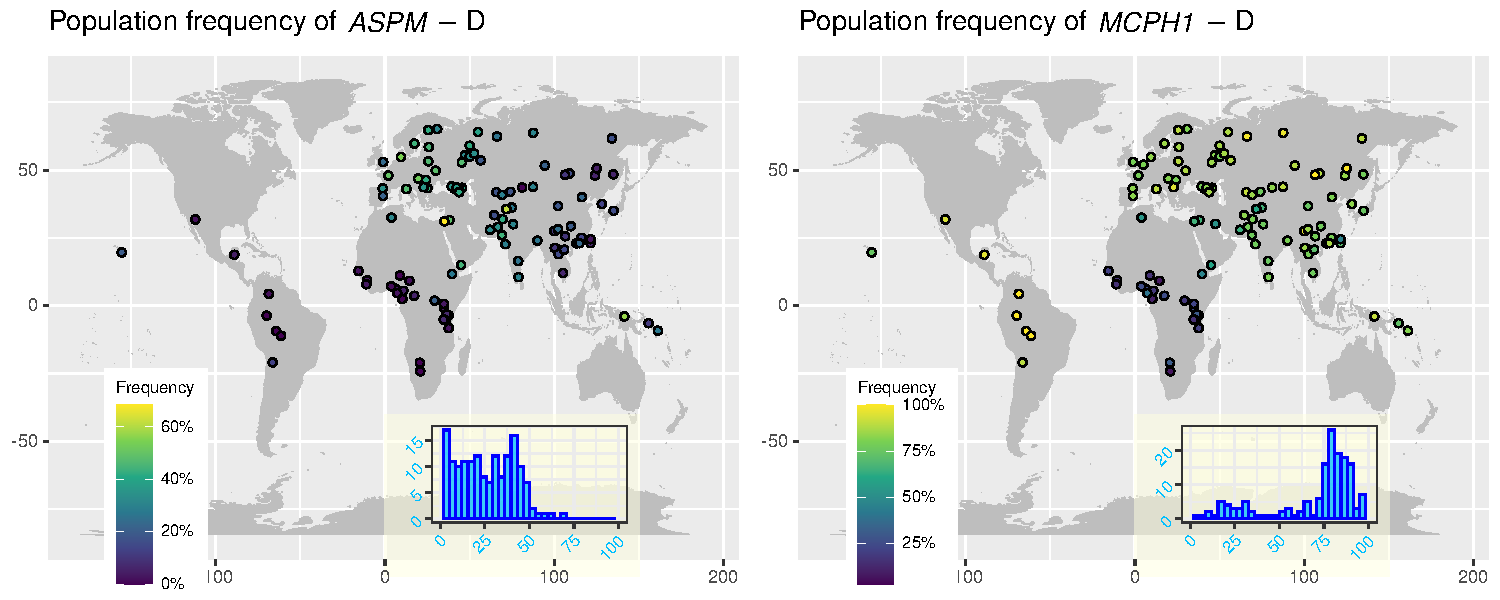
\includegraphics[width=\textwidth]{../../code/figures/map_alleles}
	\caption{The distribution of the two ``derived'' alleles in the newer data. Left: \textit{ASPM}-D, right: \textit{MCPH1}-D. Each circle on the maps represents a unique sample, and its colour represents the frequency (as the percent) of the ``derived'' allele in that sample. The inset show the overall histogram of the allele frequency across all the samples. Please note that the maximum percentage (corresponding to the lightest colour) differs between the two panels.}
	\label{Fig:gene_maps}
\end{figure}


\subsection{Tone}

\paragraph{Matching samples to languages.}

In most cases, the mapping of a given genetic sample to one (or more) language(s), using the provided metadata, is far from obvious.
To this end, I used all the available information about the sample in the data source giving the allele frequency\footnote{For example, the description of the population ``Adygei'' [\texttt{PO000017I}] in \textit{ALFRED}, available at \url{https://alfred.med.yale.edu/alfred/recordinfo.asp?UNID=PO000017I}, gives general data about the population, including links to the \textit{Ethnologue}, as well as more specific information about each particular sample, possibly including reference(s) to the actual publication(s).}, in combination with other sources such as \textit{Wikipedia} (\url{https://www.wikipedia.org}), the \textit{Ethnologue} (\url{https://www.ethnologue.com}), the \textit{Glottolog} (\url{https://glottolog.org}), \textit{WALS} (\url{https://wals.info}), and the \textit{ISO 639-3 Registration Authority} website (\url{https://iso639-3.sil.org}), plus general knowledge about the distribution of the world's languages and ethnic groups.
While this resulted in clear matches in many cases, with 139 samples (80\%) being uniquely matched to a single language (e.g., the samples of the ``Adygei'' [\texttt{PO000017I}] population were uniquely matched to the \textit{Adyghe} language, Glottocode \texttt{adyg1241}, ISO-639-3 \texttt{ady}), and 23 samples to 2 languages each (e.g., the ``Bakola Pygmy'' were mapped to either/both \textit{Gyele} [\texttt{gyel1242}, \texttt{gyi}] and \textit{Kwasio} [\texttt{kwas1243}, \texttt{nmg}]), there were also more ambiguous mappings: 4 samples mapped to 3 languages each, 4 to 3, 1 each to 5, 6, 7 and 9 languages, 1 to 23 languages (the \textit{ALFRED}/\textit{HGDP} sample \texttt{SA001501H} ``Papuan'', where the best I could do was to map it to a whole set of potential \textit{Sepik}, \textit{Ndu}, \textit{Ap Ma}, and\textit{ Lower Speik-Ramu} languages), and 1 mapping to no less than 144 languages (this ``monster'' is the \texttt{SA004382R} ``Micronesians'' sample, which could only be mapped to a whole subset of the \textit{Austronesian} family).
This ambiguous mapping introduces an extra level of uncertainty.

\paragraph{Data sources.}

I collected data from five sources (see Table \ref{Tab:tone_data_surces}).
I used the 2014 version of the \textit{WALS Online} \citep{dryer_wals_2013}, which gives tone as a 3-way classification (``Feature 13A'') in a machine-readable format (\texttt{CSV}).
I manually collected the tone data from the \textit{LAPSyD} website (\url{http://www.lapsyd.ddl.cnrs.fr/lapsyd/index.php}) in early 2020, noting, for each language, the 5-way classification and the given number of tones.
The binary classification of tone (present/absent) used in the \citet{dediu_ladd_2007} paper is available in Annex 6 of my PhD thesis (\citealp{dediu_phd_2007}, \url{https://doi.org/10.5281/zenodo.4252896}); it was manually curated from several primary and secondary sources (see \citealp{dediu_phd_2007} and \citealp{dediu_phd_2007} for details).
For \textit{PHOIBLE} \citep{moran_phoible_2014}, I downloaded the 2.0.1 version of the database and I extracted only the symbols used for tone (\texttt{SegmentClass = "tone"}), manually removing some symbols that appear only very rarely (see Figure \ref{Fig:rare_phoible_tone_symbols}).
Unfortunately, the data of \textit{The World Phonotactics Database} (\citealp{donohue_world_2013}; \textit{WPHON}) was not accessible as of April 2020, so I used instead the latest available snapshot from the Internet Archive/the WayBackMachine from 8 June 2019, available at \url{https://web.archive.org/web/20190608215845/http://phonotactics.anu.edu.au/features.php}, marked as ``Updated: 4 May 2017'', which I converted to \texttt{CSV} by adapting the \texttt{Python} script \texttt{phonotactics.py} available from \url{https://gist.github.com/xflr6/800401204fe15a6d1b9289149725b790} (\verb|download_and_convert_WPD.py|); this database gives the actual number of ``tonal contrasts'' in a language.

I also used the \textit{Glottolog} \citep{hammarstrom_glottolog_2018} version 4.1 (\url{https://glottolog.org}) for the genealogical classification of languages in \emph{language families}, and in \textit{macroareas}.


\begin{table}[h]
  \caption{Data sources for linguistic tone with the number of languages (the ``\#'' column).}
  \label{Tab:tone_data_surces}
  \centering
  \begin{tabularx}{\textwidth}{|X|X|X|r|}
    \toprule
    \textbf{Source} & \textbf{URL} & \textbf{Content} & \textbf{\#} \\
    \midrule
    \textit{WALS Online} \citep{dryer_wals_2013} & \url{https://wals.info/feature/13A} & 3-way classification: ``No tones'', ``Simple tone system'' \& ``Complex tone system''  & 513 \\
    \textit{LAPSyD} & \url{http://www.lapsyd.ddl.cnrs.fr/lapsyd/index.php} & 5-way classification: ``None'', ``Marginal'', ``Simple'', ``Moderately complex'' \& ``Complex'', as well as the actual number of tones  & 569 \\
    \textit{DL2007} \citep{dediu_ladd_2007} & \citet[Annex 6, p. 373--386]{dediu_phd_2007}; \url{https://doi.org/10.5281/zenodo.4252896} & Binary classification: ``No'' vs ``Yes''  & 60 \\
    \textit{PHOIBLE} \citep{moran_phoible_2014} & \url{https://phoible.org} & Actual tone symbols (\url{https://phoible.org/parameters})  & 2030 \\
    \textit{The World Phonotactics Database} (\textit{WPHON}) \citep{donohue_world_2013} & \url{https://web.archive.org/web/20190608215845/http://phonotactics.anu.edu.au/features.php} & Number of tones  & 3160 \\
    \bottomrule
  \end{tabularx}
\end{table}

\begin{figure}[h]
  \centering
  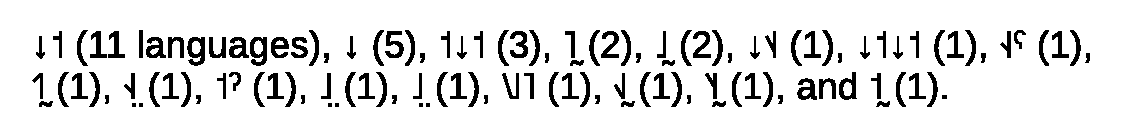
\includegraphics[width=10cm]{phoible_rare_tone_symbols}
  \caption{The tone symbols in \textit{PHOIBLE} that were removed because they appeared too rarely in the database (with the number of occurrences in parentheses).}
  \label{Fig:rare_phoible_tone_symbols}
\end{figure}


\paragraph{Tone classifications.}

Given these sources, I decided to compile information about tone in three formats (codings):

\begin{enumerate}
  \item a \emph{binary} coding, opposing languages that do not use any tone system to those that do (i.e., absence vs. presence): ``No''/''Yes'';
  \item a \emph{3-way ordered} coding of tone system complexity: ``None'' < ``Simple'' < ``Complex'';
  \item a \emph{count} of the number of tones (or tone symbols) used to describe a language, ranging from 0 (no tone) to a maximum dependent on the data source.
\end{enumerate}

The rules for obtaining these coding for each data source are given in Table \ref{Tab:tone_coding_rules}.
Please note that the counts were \emph{rebased}, in the sense that those few languages reported as having 1 tone/symbol were recoded as having 2\footnote{The fact that they are very few (6 for \textit{LAPSyD}, 4 for \textit{PHOIBLE}, and 3 for \textit{WPHON}), coupled with a case-by-case analysis, suggested that they can be safely collapsed with the languages with 2, all being considered as having simple tone systems.}, followed by the subtraction of 1 for all languages with at least 2 tones/symbols (i.e., the languages with 0 tones/symbols stay at 0, but all languages with $n \geq 2$ tones/symbols are recoded as having $n-1$ tones/symbols) -- in this way, we have a continuum of counts from 0 up to the original maximum -1.

\begin{table}[h]
  \caption{How I coded tone for each data source. The given rules are of the form \textit{original value(s)}  $\mapsto$ \textit{coded value}; $\ast$ means ``all other original value(s)''; ``as is'' means the value as given by the data source without change; ``rebase'' applies only to the counts (see text for details); ``--'' means that the data source did not contribute to the coding (does not contain useful information).}
  \label{Tab:tone_coding_rules}
  \centering
  \begin{tabularx}{\textwidth}{|r|X|X|X|}
    \toprule
    \textbf{Source} & \textbf{Binary} & \textbf{3-way} & \textbf{Count} \\
    \midrule
    \textit{WALS} & \makecell[l]{``None'' $\mapsto$ ``No''\\ $\ast \mapsto$ ``Yes''} & as is & -- \\
    \midrule
    \textit{LAPSyD} & \makecell[l]{``None'' $\mapsto$ ``No''\\ $\ast \mapsto$ ``Yes''} & \makecell[l]{``None'' $\mapsto$ ``None''\\``Marginal'' $\mapsto$ ``Simple''\\``Simple'' $\mapsto$ ``Simple''\\ $\ast \mapsto$ ``Complex''} & rebase \\
    \midrule
    \textit{DL2007} & as is & -- & -- \\
    \midrule
    \textit{PHOIBLE} & \makecell[l]{0 $\mapsto$ ``No''\\ $\ast \mapsto$ ``Yes''} & \makecell[l]{0 $\mapsto$ ``None''\\ $\leq 2 \mapsto$ ``Simple''\\ $\ast \mapsto$ ``Complex''} & rebase \\
    \midrule
    \textit{WPHON} & \makecell[l]{0 $\mapsto$ ``No''\\ $\ast \mapsto$ ``Yes''} & \makecell[l]{0 $\mapsto$ ``None''\\ $\leq 3 \mapsto$ ``Simple''\\ $\ast \mapsto$ ``Complex''} & rebase \\
    \bottomrule
  \end{tabularx}
\end{table}

\paragraph{Reconciliation of the sources.}

While the agreement between these five sources is very good (see Supplementary materials \ref{SM:tone_agreeemnt_sources}), there are some languages for which they disagree (e.g., \textit{Angaataha} [\texttt{anga1290}, \texttt{agm}] is coded as ``Moderately complex'' in \textit{LAPSyD}, but as ``Simple'' in \textit{WALS}).
Moreover, few languages are coded in all sources.
Therefore, it would be preferable to arrive at an \emph{agreement} coding of tone that (a) reconciles any existing conflicts and (b) can retain as many languages as possible.
To this end, I implemented the following algorithm.

\paragraph{For the categorical classifications (binary and 3-way),}
I implemented a set of rules based on a hierarchy of the sources and the pattern of agreements and disagreements between them; while still subjective, this is fully replicable, transparent and can be easily modified.
I preferred to use manually-curated categorical classifications over the count-level sources, resulting in the following (rough) ordering in terms of precedence: \textit{LAPSyD} $\geq$ \textit{WALS} $\geq$ \textit{DL2007} $\geq$ \textit{WPHON} $\geq$ \textit{PHOIBLE}.
The actual rules are coded as patterns of information about a given language in the available sources and the actions to be taken (e.g., if a language has information in \textit{LAPSyD}, then this is used no matter what other information is available); in this way, the coding conflicts are implicitly solved by picking the ``highest'' available source.

\paragraph{For the counts,}
I used a similar approach, in that the sources are ordered as \textit{LAPSyD} $\geq$ \textit{WPHON} $\geq$ \textit{PHOIBLE}, with the added twist that for the last two (\textit{WPHON} and \textit{PHOIBLE}) I do not pick the ``raw'' value as given by the database itself, but instead a ``corrected'' value.
More exactly, given that I consider the tone counts in \textit{LAPSyD} as the ``gold standard'', I performed first the quadratic regression of the \textit{LAPSyD} counts on the \textit{WPHON} counts and, separately, on the  \textit{PHOIBLE} counts, and used the (rounded) value predicted by these regression models from the ``raw'' value in the corresponding database.
These regressions are:
$$L = 0.08 (\pm0.04) + 0.92 (\pm0.06)W - 0.04 (\pm0.01)W^2$$
$$L = 0.39 (\pm0.05) + 0.68 (\pm0.09)P - 0.04 (\pm0.02)P^2$$
where $L$ is the predicted \textit{LAPSyD} count from the ``raw'' \textit{WPHON} ($W$) or \textit{PHOIBLE} ($P$) count.
This procedure attempts to ``align'' and ``scale'' the counts (also allowing a non-linear quadratic term) so that they better map between sources.

\paragraph{The \emph{agreement} classification.}
With these, I obtained three agreement classifications (one binary, one 3-way, and one count), that agree very well with the original sources (see Supplementary materials \ref{SM:tone_agreeemnt_with_sources}).
These have the following distributions (see also Figure \ref{Fig:map_tone}):

\begin{itemize}
  \item \emph{binary}: ``No'' (251), and ``Yes'' (70);
  \item \emph{3-way}: ``None'' (242), ``Simple'' (36), and ``Complex'' (22);
  \item \emph{counts}: ``0'' (249), ``1'' (26), ``2'' (23), ``3'' (6), ``4'' (5), ``5'' (3), and ``6'' (2).
\end{itemize}

\begin{figure}[h]
  \centering
  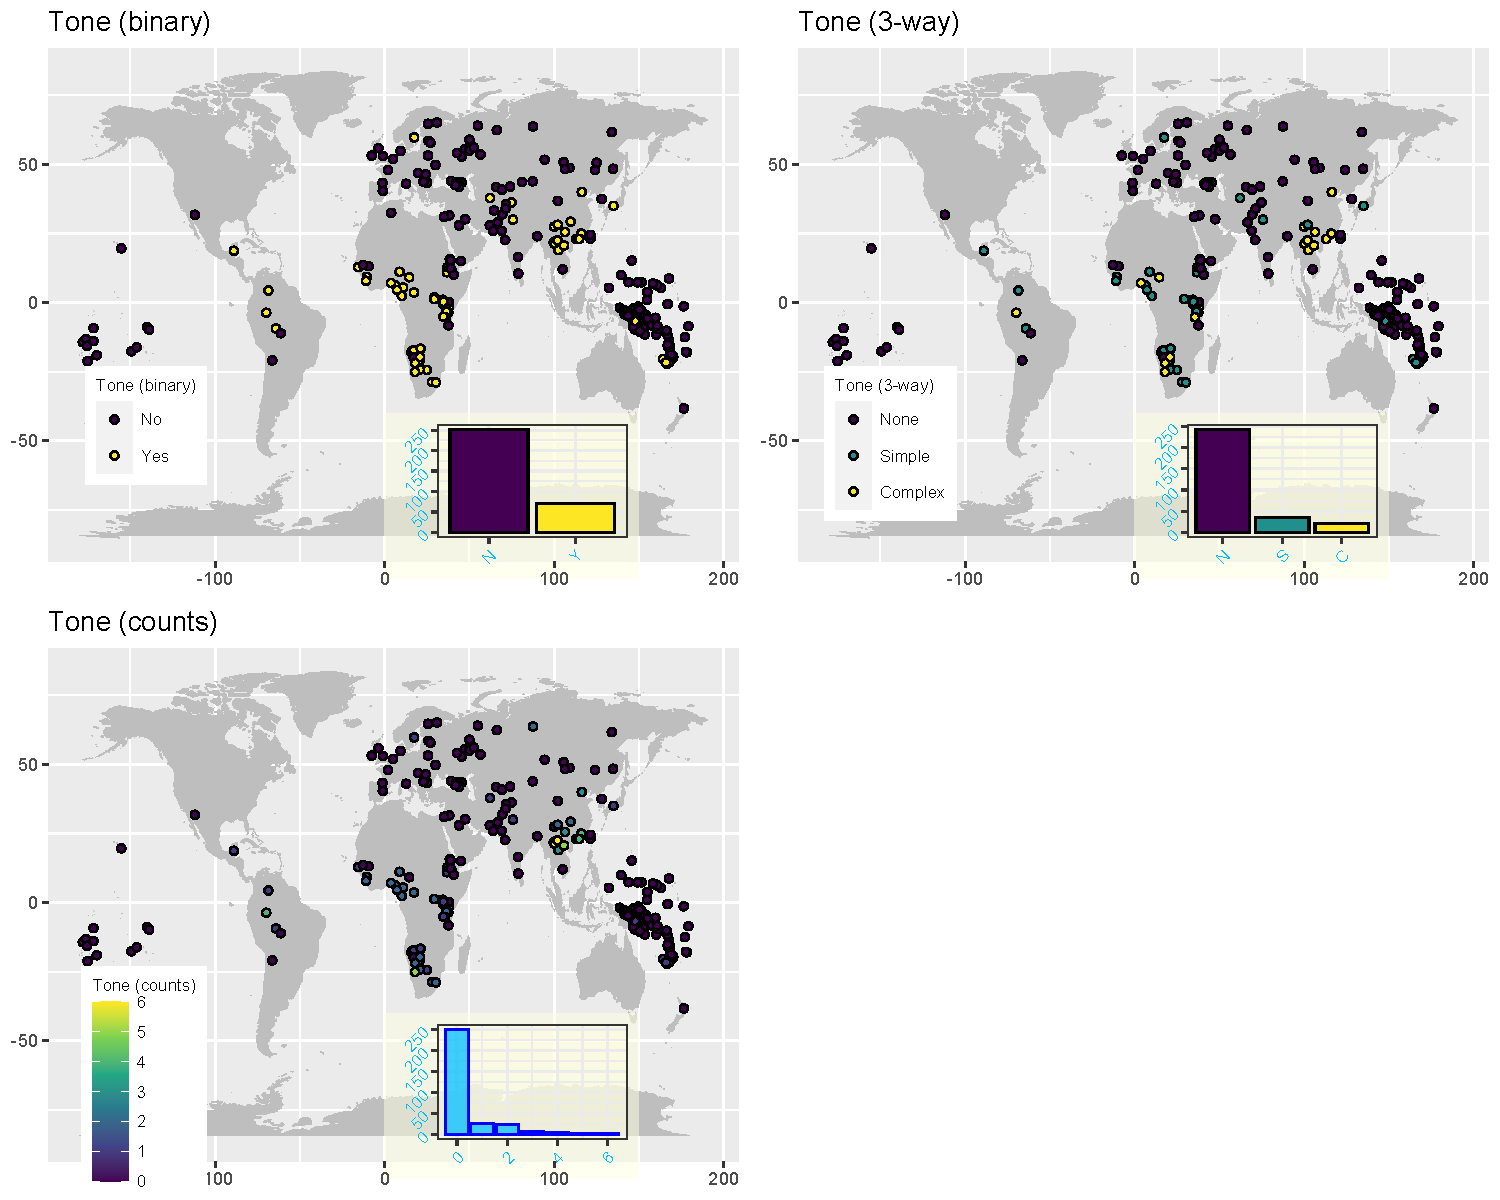
\includegraphics[width=\textwidth]{../../code/figures/map_tone}
  \caption{The distribution of the agreement tone. Each circle on the maps represents a unique language, and its colour represents is value. The insets show the overall distributions across all the languages. Top-left: binary tone (inset horizontal axis: ``N'' = ``No'', ``Y'' = ``Yes''); top-right: 3-way classification (inset horizontal axis: ``N'' = ``None'', ``S'' = ``Simple'', ``C'' = ``Complex''); bottom-left: tone counts.}
  \label{Fig:map_tone}
\end{figure}

For the purposes of the analyses reported here, I considered the following variables referring to tone:

\begin{itemize}
  \item \emph{tone1}: this is a shorter name for the binary coding of tone as ``No'' (251) vs ``Yes'' (70);
  \item \emph{tone2}: this is a binary variable derived from the 3-way coding of tone by opposing ``Complex'' tone systems (coded as ``Yes'', 22 languages) vs ``None'' and ``Simple'' collapsed together (coded as ``No'', in 278 languages);
  \item \emph{counts}: the unchanged tone counts from above.
\end{itemize}



%------------------------------------------------

\section{Methods}

I analysed separately the three variables related to tone, namely \textit{tone1}, \textit{tone2} and tone \textit{counts}.
For each variable, I selected only the entries with non-missing data for it as well as for the two ``derived'' alleles; if, for a given sample, there is more than one possible language or allele frequencies, I only kept those entries that have different tone and/or allele information.
This procedure maintains the uncertainty in the data, and while it might be seen as giving too much voice to ``exceptions'', it avoids giving too much voice to entries that happen to be similar due to close genealogical relatedness.
With these, there are 181 observations among 119 unique Glottolg codes in 35 families for \textit{tone1}, 165 observations among 108 unique Glottolg codes in 35 families for \textit{tone2}, and 184 observations among 121 unique Glottolg codes in 35 families for tone \textit{counts}.


\subsection{Modelling (meta)populations, macroareas and families}

As the \emph{(meta)populations} are fully included in the language families, and most have just a few samples\footnote{Of the 129 unique (meta)populations, 100 have only 1 sample, 17 have 2 samples, 8 have 3, 3 (``Finns'', ``Jews\_Ashkenazi'' and ``Russians'') have 4, and there is only 1 (``Han'') with 5 samples.}, I did not explicitly model them here, as they add too little information to the samples and the language families.

However, the \emph{families} do need to be considered (even if most have only one or a few languages\footnote{Of all the 39 unique families, 16 are represented by a single language, 6 by 2, 5 by 3, 3 by 5, 2 by 7, 3 by 10, and 1 each by 16 (``Afro-Asiatic''), 26 (``Indo-European''), 31 (``Atlantic-Congo'') and 146 (``Austronesian'') languages, respectively.}), as it is essential to properly model the genealogical non-independence between related languages: therefore, I modelled them as \emph{random effects} (in the now standard approach; e.g. \citealp{ladd_correlational_2015}).

\emph{Macroareas}, on the other hand, need special consideration for several reasons:

\begin{itemize}
  \item there is a very skewed geographical sampling (e.g, there is nothing from Australia, and very few data points from the Americas), the dataset being dominated by Eurasia and Africa;
  \item the macroareas (as defined in the \textit{Glottolog}) have, in fact, a pretty unclear status, being probably more justified geographically (``continents'') but arguably less so from the linguistic, anthropological and historical points of view (e.g, ``Africa'' and ``Eurasia'' are treated as unitary, while PNG and Oceania are placed together within ``Papunesia'');
  \item the distribution of the two ``derived'' alleles is also highly skewed geographically, being almost completely absent from Africa.
\end{itemize}

Therefore,

\begin{itemize}
  \item as ``North America'' and 'South America'' each have very few data points, I collapsed them into a single macroarea, ``America'';
  \item in order to control for the influence of the macroareas, I modelled them as \emph{fixed effects};
  \item because the genetic data suggests that the major split is between ``Africa'' and the rest of the world, coupled with the fact that some methods cannot gracefully handle multi-valued factors, made me dichotomise, for some analyses, macroarea in into ``Africa'' vs ``non-Africa''.
\end{itemize}


\subsection{Operationalization of the hypotheses}

Following \citet{dediu_ladd_2007} and \citet{ladd_bioling_2008}, and the direct experimental tests in \citet{wong_plosone_2012} and \citet{wong_sciadv_2020}, I am testing here the following hypotheses:

\begin{itemize}
  \item there is a \textbf{weak negative influence} of the population frequency of \textit{ASPM}-D on \textit{tone1} above and beyond the effects of shared ancestry (\textit{language family}) and contact (\textit{macroarea});
  \item there should be \textbf{no effect} of \textit{MCPH1}-D on \textit{tone1} independent of \textit{language family} and \textit{macroarea}, or it should be much smaller.
\end{itemize}

There are no clear predictions concerning the complexity of tone systems (\textit{tone2} and tone \textit{counts}), but we might expect a negative effect of \textit{ASPM}-D:

\begin{itemize}
  \item there might be a \textbf{weak negative influence} of \textit{ASPM}-D on \textit{tone2} above and beyond \textit{language family} and \textit{macroarea};
  \item there might be a \textbf{weak negative influence} of \textit{ASPM}-D on tone \textit{counts} above and beyond \textit{language family} and \textit{macroarea};
  \item there is \textbf{no particular influence} of \textit{MCPH1}-D on \textit{tone2} independent of \textit{language family} and \textit{macroarea};
  \item there is \textbf{no particular influence} of \textit{MCPH1}-D on tone \textit{counts} independent of \textit{language family} and \textit{macroarea}.
\end{itemize}


\subsection{Throwing the causal baby with the confounding bathwater?}

However, the ``above and beyond the effects of shared ancestry (\textit{language family}) and contact (\textit{macroarea})'' are rather tricky in this particular case, and should be treated with care.
These are indeed potential confounds in any cross-linguistic/cross-cultural/cross-population statistical studies and usually result in artificially inflated (i.e., artificially statistically significant) associations \citep{ladd_correlational_2015}.
This is due to the fact that the languages/cultures/populations are not statistically independent, but more similar than expected by chance due to ``genealogical inertia'' (``Galton's problem''; \citealp{mace_galtonproblem_1994}) and contact.
In our case, tone seems to be both stable genealogically (i.e., the daughter languages have a strong tendency to conserve the tonal system of their proto-language) and relatively easy to borrow between neighbouring languages \citep{yip_tone_2002,dediu_procb_2011,dediu_cysouw_2013,kauhanen_geospatial_2018,collins_tone_2016}.
Likewise, given that the two ``derived'' alleles, \textit{ASPM}-D and \textit{MCPH1}-D, are very probably evolving neutrally \citep{currat_comment_2006}, it is to be expected that their frequencies in any given population are shaped by drift and admixture \citep{jobling_human_2013}.
While in small isolated populations their frequency might fluctuate widely across generations (possibly ending in fixation or complete loss), in larger ones they are expected to be relatively stable.
Moreover, genetic exchanges between populations (due to inter-marriage, migrations...) lead to more similar frequencies, while various barriers (physical or cultural) might lead to increased differentiation \citep{jobling_human_2013,reich_who_2018}.
Thus, any apparent association between tone and the frequency of the ``derived'' alleles in present-day populations might be \emph{non-causal} but \emph{spurious}, due to a fortuitous accident through which it just so happened that a few populations, some generations ago, had a high frequency of the ``derived'' alleles and no tone, accident later amplified by language expansions, demographic processes and contact, making the proper control for these non-independencies a must \citep{roberts_traffic_2013,ladd_correlational_2015}.

On the other hand, if the hypothesis that the ``derived'' alleles induce a weak individual bias that can be amplified by the repeated use and transmission of language across multiple generations \citep{dediu_ladd_2007,dediu_humbiol_2011,ladd_bioling_2008} is true (as strongly suggested by the experimental evidence; \citealp{wong_plosone_2012,wong_sciadv_2020}), then the cross-linguistic/cross-population effects of this \emph{causal} link might look very similar to the very confounds discussed above.
This is so because in populations with a low frequency of the ``derived'' alleles, tone is ``free'' to change (i.e., being innovated, complexified, simplified or lost) under the influence of other processes (internally-motivated sound change, language contact, or even climate; \citealp{yip_tone_2002,hombert_tone_1979,everett_language_2016}), but in populations with a higher frequency of these alleles, there is an extra (weak) force against tone (thus, either a ``push'' away from tone through increased rates of tone simplification and loss, or a ``pull'' towards a lack of tone through a low probability of tonogenesis).
The effects of this ``extra'' force (the \emph{negative bias}) would not be instantaneous, but would presumably require several generations.

There are four important scenarios to analyse: in the first, there is a significant \emph{increase}\footnote{Please note that it is currently unclear what a ``significant'' change in the frequency of the ``derived'' alleles should be, if this change is independent or not of the frequency itself, if there are thresholds or more general non-linearities, and if the frequency is modulated by the structure of the communicative network itself \citep{dediu_jtb_2008,dediu_jtb_2009,josserand_frontiers_2020} -- all in need of specific computational and cross-linguistic work that go beyond the scope of this paper; for my purposes here suffices that there are changes in allele frequency that result in changes in the negative bias towards tone at the language level.} in the frequency of the ``derived'' alleles (due to drift or gene flow), in the second there is a \emph{stable high} frequency of the alleles, in the third, there is a significant \emph{decrease} in this frequency, and in the fourth, a \emph{stable low} frequency of the alleles.

In the first scenario, when the frequency of the ``derived'' alleles increases sufficiently in a population so that the negative bias becomes active, then we would expect that the original language(s) of the population would start simplifying or losing tone (if they had it), or fail to develop or complexify it (even if other conditions hold).
If this process is on the same timescale as language differentiation or faster (a few generations/hundreds of years), it might retrospectively look like a ``regular'' sound change (or, even much harder to ascertain, a failure to change despite favouring conditions), followed (second scenario) by a period of relative stability (lack of tone) across the history of the ensuing language family.
Moreover, given that it is highly improbable that such significant changes in allele frequency happen just in a single population that is large enough to support a viable language, or that it would stay confined there, they would likely affect (relatively simultaneously), or spread among, bigger groups of people speaking multiple languages across larger areas; retrospectively, this might look like a period of tone simplification or loss among several languages in contact which can be interpreted as contact-induced, followed by a period of relative stable lack of tone (second scenario).

In contrast, in the third scenario, the frequency of the ``derived'' alleles decreases sufficiently to remove the negative bias against tone, ``allowing'' the other forces to resume affecting tone, effectively ``opening'' up tonogenesis and tone complexification as possible pathways of language change, possibly followed by the fourth scenario, where the frequency of the ``derived'' alleles is low and the negative bias inactive.
Retrospectively, scenario three would be hard to distinguish from the ``usual'' evolution of tone systems, except by being preceded by a period characterised by a lack of tone in the history of the languages.
Scenario four is that of language change ``as usual'' in the absence of a genetic bias, where tone is gained and lost, complexified and simplified as driven by other factors.

Given what we know about the two ``derived'' alleles, namely that they emerged relatively recently (\textit{ASPM}-D $\approx$ 6,000 years ago, and \textit{MCPH1}-D $\approx$ 37,000 years ago) presumably somewhere in Eurasia, and have since spread and increased in frequency (presumably due to demographic processes of expansion, migration and inter-marriage) slowly and unequally around the globe, it is probable that all scenarios are applicable in different circumstances (linguistic families and geographic areas), but that scenario three is rather improbable.

Thus, because of the intrinsic population dynamics of these ``derived'' alleles, of the weakness of the bias they produce, and of the complex multi-factorial nature of language change (combining many types of influences and a good dose of serendipity), the causal effects of this bias will largely overlap with those of genealogical inertia (because, just as tone, the allele frequencies of the daughter populations are highly correlated between them and with those of the mother population) and areal effects/language contact (because, just as tone, the ``derived'' alleles are spread by people moving and interacting with each other).
Figure \ref{Fig:dag_tone_genes} is a representation of these relationships using Judea Pearl's Directed Acyclic Graph (DAG) approach to causality \citep{pearl_causality_2000,pearl_why_2018,mcelreath_statistical_2020}.

\begin{figure}[h]
  \centering
  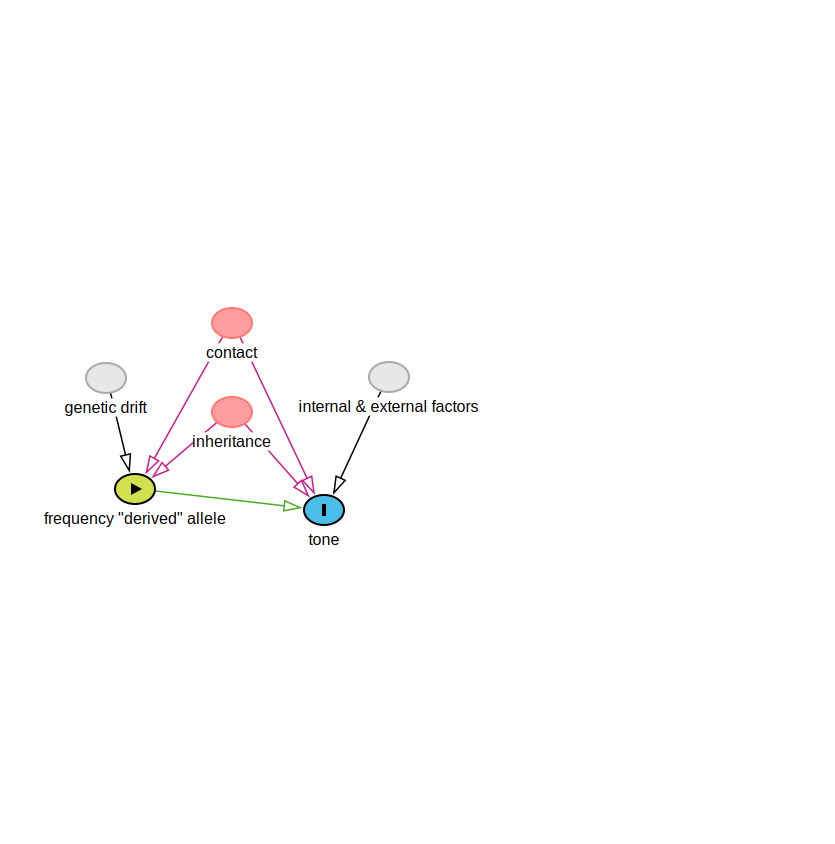
\includegraphics[width=0.75\textwidth]{dag_tone_genes}
  \caption{Simplified model of the causal and spurious relationships between the frequency of the ``derived'' alleles (the \textit{exposure}) and tone (the \textit{outcome}) using Directed Acyclic Graphs (DAGs). The arrows represent direct causal effect; the grey nodes are unmeasured variables.}
  \label{Fig:dag_tone_genes}
\end{figure}


\subsection{Statistical methods}

Given the limitations of the data available (nut only in terms of sample size, but also of geographic and linguistic representativeness and ambiguity) and the complexity of the casual model and the role of inheritance and contact discussed above, I used multiple methods to try to test these hypotheses.

I decided against the use of Bayesian regression models (as implemented, for example, by \texttt{R}'s \texttt{brms} package or directly using \texttt{Stan}) due to their very similar results to the ``classic'' implementations (as available through (\texttt{g})\texttt{lmer} and \texttt{glmmTMB}) but at much lower computational costs, especially important for the randomisation and restricted sampling approaches.
For \textit{tone1} and \textit{tone2} (binary variables) I performed logistic regressions (as implemented by \texttt{glm} and \texttt{glmer} when there is no random structure and where there is one, respectively), for the tone \textit{counts} I used Poisson regression (\texttt{glmer}), and for the population frequencies of the ``derived'' alleles I used Beta regression (as implemented by \texttt{glmmTMB}, but replacing all $0.0$ values with $10^{-7}$ and all $1.0$ values with $1.0 - 10^{-7}$, respectively).

\paragraph{(Mixed-effects) regressions.}

This implements the largely current ``standard'' approach in cross-linguistic studies, where the dependent variable (DV) is regressed on the independent variable(s) (IVs), while the potential confounds are modelled as fixed or random effects \citep{ladd_correlational_2015,jaeger_mixed_2011}.
In particular, here the DV is either \textit{tone1}, \textit{tone2} or \textit{counts}, and the IVs of interest are the population frequencies of \textit{ASPM}-D and \textit{MCPH1}-D (and their interaction), while the confounds are \textit{macroarea} (fixed effect) and its interactions with \textit{ASPM}-D and \textit{MCPH1}-D, and language \textit{family} (random effect).
I individually tested the significance of each fixed effect separately by performing a likelihood ratio test and comparing the Akaike Information Criteria (AIC) between the model with the fixed effect of interest and the model without it.
For each DV:

\begin{description}
  \item[all data:] I first fitted the regression model on all the available data;
  \item[randomization:] followed by a permutation approach where I repeatedly ($n = 1000$) shuffle the data and re-fit the regression model, resulting in a null distribution of model fits that can be compared to the original fit to the unshuffled data. In fact, there are 18 different scenarios resulting from combinations of three parameters that test slightly different null hypotheses (see Tables \ref{Tab:randomization_params} and \ref{Tab:randomization_scenarios});
  \item[restricted sampling:] finally, a popular approach in typology is represented by sampling only one language from each genealogical and/or areal unit \citep{dryer_sampling_areas_1989,bakker_sampling_language_2010,everett_climate_2015}, which I implemented here by repeatedly picking only one language from each family, fitting a regression model (without any random effects structure, as each family now has exactly one member) while controlling or not for macroarea, and analysing the distribution of the model fits (this time, the comparison is done against the null hypothesis of no effect).
\end{description}

\begin{table}[h]
  \caption{The parameters of the randomisation approach, defining, on the one hand, what is permuted and within what constraints, and what to control for in the regression models, on the other.}
  \label{Tab:randomization_params}
  \centering
  \begin{tabularx}{\textwidth}{|r|X|r|}
    \toprule
    \textbf{Parameter} & \textbf{Meaning} & \textbf{Possible values} \\
    \midrule
    \textit{permute} & what is permuted & \makecell[l]{\textit{tone} = permute the tone variable\\~~~~$\rightarrow$ destroys the patterning of tone\\
      \textit{alleles-together} = permute the two alleles together\\~~~~$\rightarrow$ destroys the patterning of the two ``derived''\\~~~~ alleles but not the correlation between them\\
      \textit{alleles-independent} = permute the two alleles independently\\~~~~$\rightarrow$ destroys the patterning of the two ``derived''\\~~~~ alleles and the correlation between them} \\
    \midrule
    \textit{within} & constraints on permutations & \makecell[l]{\textit{unrestricted} = all observations are freely permuted\\~~~~$\rightarrow$ destroys all structure in the data\\
      \textit{families} = observations are permuted within their family\\~~~~$\rightarrow$ destroys the within-family structure,\\~~~~ but conserves the between-families variation\\~~~~ i.e., conserves the genealogical signal\\
      \textit{macroareas} = observations are permuted within their macroarea\\~~~~$\rightarrow$ destroys the within-area structure,\\~~~~ but conserves the between-areas variation\\~~~~ i.e., conserves the areal (contact) signal} \\
    \midrule
    \textit{macroarea} & is there control for macroareas? & \makecell[l]{\textit{none} = no control at all\\
      \textit{fixef} = yes, as fixed effect} \\
    \bottomrule
  \end{tabularx}
\end{table}

\begin{table}[h]
  \caption{The 18 randomisation scenarios. Parameter names and values (columns 2--3) are defined in Table \ref{Tab:randomization_params}, Name (1\textsuperscript{st} column) is a 3-letter shorthand: 1\textsuperscript{st} letter: T=tone, L=alleles-together (``linked'') and I=alleles-independent (``independent''); 2\textsuperscript{nd} letter: U=unrestricted, M=macroareas, F=families; 3\textsuperscript{rd} letter: N=none, F=fixef. --''-- means as above.}
  \label{Tab:randomization_scenarios}
  \centering
  \begin{tabularx}{\textwidth}{|l|l|l|l|X|}
    \toprule
    \textbf{Name} & \textbf{Permute} & \textbf{Within} & \textbf{Macroarea} & \textbf{Interpretation} \\
    \midrule
    TUN & \textit{tone} & \textit{unrestricted} & \textit{none} & tone is permuted across the whole sample $\rightarrow$ destroys the family and macroarea structure of tone, but keeps it for the alleles; macroarea is not included \\
    \midrule
    LUN & \textit{alleles-together} & \textit{unrestricted} & \textit{none} & the frequencies of the two ``derived'' alleles are permuted across the whole sample together $\rightarrow$ destroys the family and macroarea structure of the two alleles (while preserving correlations between them), but keeps it for tone; macroarea is not included \\
    \midrule
    IUN & \textit{alleles-independent} & \textit{unrestricted} & \textit{none} & the two alleles are permuted across the whole sample independently $\rightarrow$ destroys the family and macroarea structure of the two alleles and the correlations between them, but keeps it for tone; macroarea is not included \\
    \midrule
    TUF & \textit{tone} & \textit{unrestricted} & \textit{fixef} & as TUN but controlling for macroarea \\
    LUF & \textit{alleles-together} & \textit{unrestricted} & \textit{fixef} & as LUN --''-- \\
    IUF & \textit{alleles-independent} & \textit{unrestricted} & \textit{fixef} & as IUN --''-- \\
    \midrule
    TMN & \textit{tone} & \textit{macroareas} & \textit{none} & as TUN but only data points from the same macroarea are permutted \\
    LMN & \textit{alleles-together} & \textit{macroareas} & \textit{none} & as LUN --''-- \\
    IMN & \textit{alleles-independent} & \textit{macroareas} & \textit{none} & as IUN --''-- \\
    \midrule
    TMF & \textit{tone} & \textit{macroareas} & \textit{fixef} & as TMN but controlling for macroarea \\
    LMF & \textit{alleles-together} & \textit{macroareas} & \textit{fixef} & as LMN --''-- \\
    IMF & \textit{alleles-independent} & \textit{macroareas} & \textit{fixef} & as IMN --''-- \\
    \midrule
    TFN & \textit{tone} & \textit{families} & \textit{none} & as TUN but only data points from the same family are permutted \\
    LFN & \textit{alleles-together} & \textit{families} & \textit{none} & as LUN --''-- \\
    IFN & \textit{alleles-independent} & \textit{families} & \textit{none} & as IUN --''-- \\
    \midrule
    TFF & \textit{tone} & \textit{families} & \textit{fixef} & as TFN but controlling for macroarea \\
    LFF & \textit{alleles-together} & \textit{families} & \textit{fixef} & as LFN --''-- \\
    IFF & \textit{alleles-independent} & \textit{families} & \textit{fixef} & as IFN --''-- \\
    \bottomrule
  \end{tabularx}
\end{table}

\paragraph{Mediation and path analysis.}

Because \textit{macroarea}, and especially its dichotomisation as Africa vs the rest of the world, predicts both the distribution of tone and the frequency of the two ``derived'' alleles, it confounds any potential causal effect that the alleles may have on tone.
\emph{Mediation analysis} \citep{mackinnon_mediation_2007} allows the partitioning of the \emph{total effect} (TE) of a variable of interest (here, \textit{macroarea}) on the outcome (here, tone) into its \emph{direct effect} (ADE) and its \emph{mediated} (or indirect) \emph{effect} (ACME), the latter being ``channelled'' through a mediator variable (here, \textit{ASPM}-D or \textit{MCPH1}-D) -- see Figure \ref{Fig:mediation_analysis}.
I performed the mediation analysis using the \texttt{R} package \texttt{mediation}, using logistic regressions for \textit{tone1} and \textit{tone2}, linear regressions for \textit{ASPM}-D and \textit{MCPH1}-D, and Poisson regression for tone \textit{counts}.

\tikzset{every picture/.style={line width=0.75pt}} %set default line width to 0.75pt
\begin{figure}[h]
  \centering

  \begin{tikzpicture}[node distance=2.0cm]
    \node(iv) {$IV$};
    \node(dv)[right of=iv] {$DV$};
    \node(mv)[above of=dv] {$MV$};
    \draw[->] (iv) -- (dv) node[midway, above] {$c'$};
    \draw[->] (iv) -- (mv) node[midway, above] {$a$};
    \draw[->] (mv) -- (dv) node[midway, right] {$b$};
  \end{tikzpicture}

  \caption{Visual representation of the mediation model. \textit{IV} is the independent variable (here, dichotomised \textit{macroarea}: inside vs outside Africa), \textit{DV} is the outcome of interest (here, the various codings of tone, \textit{tone1}, \textit{tone2} or tone \textit{counts}), and \textit{MV} is the mediator (here, the population frequency of one of the ``derived'' alleles, \textit{ASPM}-D or \textit{MCPH1}-D). The average direct effect $ADE = c'$, the average indirect effect $ACME = a \times b$, and the total effect is their sum, $TE = ADE + ACME = c' + a \times b$. The coefficients $a$, $b$ and $c'$ are obtained from fitting two regression models simultaneously (in \texttt{R} formula notation): $DV \sim IV + MV$ and $MV \sim IV$.}
  \label{Fig:mediation_analysis}
\end{figure}

\emph{Path analysis} \citep{kline_principles_2011} is even more flexible, here allowing the simultaneous modelling of the mediation effects of both ``derived'' alleles simultaneously besides the direct effect of \textit{macroarea} on tone.
Again, the \textit{macroarea} was dichotomised as Africa vs the rest of the world, but due to the limitations of the \texttt{lavaan} package, the binary \textit{IV} (the dichotomised \textit{macroarea}) and the binary \textit{DV} (\textit{tone1} and \textit{tone2}) were coded either as numeric (0 vs 1; ``rest of the world''=0, ``Africa''=1, and ``No''=0, ``Yes''=1) or as ordered categorical (``rest of the world'' < ``Africa'', and ``No'' < ``Yes''), while tone \textit{counts} were considered numeric -- please see Figure \ref{Fig:path_analysis}.

\begin{figure}[h]
  \centering

  \begin{tikzpicture}[node distance=2.0cm]
    \node(iv) {$IV$};
    \node(dv)[right of=iv] {$DV$};
    \node(m1)[above of=dv] {$MV_1$};
    \node(m2)[below of=dv] {$MV_2$};
    \draw[->] (iv) -- (dv) node[midway, above] {$c'$};
    \draw[->] (iv) -- (m1) node[midway, above] {$a_1$};
    \draw[->] (m1) -- (dv) node[midway, right] {$b_1$};
    \draw[->] (iv) -- (m2) node[midway, above] {$a_2$};
    \draw[->] (m2) -- (dv) node[midway, right] {$b_2$};
  \end{tikzpicture}

  \caption{Visual representation of the path model showing the $IV$ (Africa vs the rest of the world), the $DV$ (tone) and the two mediators $MV_1$ and $MV_2$ (\textit{ASPM}-D and \textit{MCPH1}-D), as well as all the path coefficients ($a_1$, $a_2$, $b_1$, $b_2$ and $c'$). }
  \label{Fig:path_analysis}
\end{figure}

Both the mediation and path analyses have trouble modelling the language family as a random effect, so, for each DV and type of model:

\begin{description}
  \item[all data:] I first fitted the model on all the available data, where there is no control for \textit{family};
  \item[restricted sampling:] I repeatedly fitted the model to a reduced dataset obtained by picking only one language from each family, the resulting distribution of model fits controlling thus for family.
\end{description}

(Please note that I do not need to control for \textit{macroarea}, as it is explicitly modelled as the IV.)


\paragraph{Decision trees and random forests.}

For the two binary outcomes, \textit{tone1} and \textit{tone2}, I also implemented two classification techniques widely used in machine learning, \emph{decision trees} and \emph{random forests}.
Both are used to find the subset of predictors and rules that best predict the binary outcome, and result not only in measures of how well the model fits/predict the data, but also in a set of explicit rules (decision trees) and ranking of how important the predictors are (random forests).

The measures of fit that I am using are \emph{accuracy}, \emph{sensitivity} (or \emph{recall}), \emph{specificity} and \emph{precision}; Given the observed (true) binary outcome and the model's predictions (i.e., what the model ``thinks'' or ``labels as''), the relationship between the two is described by four measures:

\begin{itemize}
  \item the number of \emph{true positives} (TP): observation and prediction agree on ``Yes'',
  \item the number of \emph{true negatives} (TN): observation and prediction agree on ``No'',
  \item the number of \emph{false positives} (FP): observation is ``No'' but prediction is ``Yes'',
  \item the number of \emph{false negatives} (FN): observation is ``Yes'' but prediction is ``No''.
\end{itemize}

With these, the total number of observations $N = (TP+FP+FN+TN)$, and:

\begin{itemize}
  \item $accuracy = (TP+TN)/N$, i.e., what proportion of observations were correctly labelled (= true positives and true negatives) by the model?
  \item $sensitivity = TP/(TP+FN)$, i.e., what proportion of the actual ``Yes'' observations (= true positives and false negatives) are labelled ``Yes'' (= true positives)?
  \item $specificity = TN/(TN+FP)$, i.e., what proportion of the actual ``No'' observations (= true negatives and false positives) are labelled ``No'' (= true negatives)?
  \item $precision = TP/(TP+FP)$, i.e., what proportion of the observations labelled ``Yes'' (= true positives and false positives) are actually ``Yes'' (= true positives)?
\end{itemize}

Ideally, these measures of fit should be close to 100\%, but deviations point to different types of failures and biases.

One important issue for such models is \emph{overfitting}, where the model ``overlearns'' the data, fitting it very well, but does very poorly at predicting new, unseen observations generated by the same processes.
One popular technique to overcome this is to repeatedly split the original dataset into two complementary subsets: a training and a testing one.
While the training subset is usually larger and is used to fit the model, the testing subset contains observations not yet ``seen'' by the model, and is used to estimate the fit measures that capture the capacity of the model to generalise to new situations.
Here I used an 80\%:20\% split of the observations between training and testing, stratified by \textit{macroarea} (i.e., making sure that the distribution of the observations in each subset reflects the distribution of the observations by macroareas in the full dataset), repeated 100 times.
Please note that because the random forests have an internal bootstrap mechanism, this repeated training/testing procedure was not applied to them.

The decision trees were implemented by \texttt{ctree} in \texttt{R}'s package \texttt{partykit}, while for random forests I used \texttt{randomForest} in package \texttt{randomForest} as well as the conditional random forests implemented by \texttt{cforest} in package \texttt{partykit}.
\texttt{randomForest} provides two measures of relative variable importance: one is based on the mean decrease in accuracy if the variable is permuted, while the second is based on the mean decrease in node impurity (measured by the Gini index) when splitting on the variable; while the first captures how much a variable helps in making accurate predictions, the second focuses on producing more homogeneous splits.
For \texttt{cforest}, I used the unconditional variable importance, which is similar to the mean decrease in accuracy.

Finally, given the importance of the \textit{macroarea} as a confound, I fitted these models with and without \textit{macroarea} as a predictor.
(Please note that these models do not control for language family at all.)


%------------------------------------------------

\section{Results}

The results are presented by outcome and method.


\subsection{The ''derived'' alleles are structured by macroarea and family}

Before we analyse the relationships between the population frequencies of the ``derived'' alleles and tone, it is important to understand how they are structured by macroarea (a proxy for contact) and language family (a proxy for genealogy).
To this end, I regressed \textit{ASPM}-D and \textit{MCPH1}-D separately on \textit{macroarea} (as fixed effect) using mixed-effects beta regression with \textit{family} as random effect\footnote{\label{note_reg_R}In \texttt{R} notation: $a \sim 1 + M + (1 \mid F)$ and $m \sim 1 + M + (1 \mid F)$, where $a$ is the population frequency of \textit{ASPM}-D and $m$ of \textit{MCPH1}-D, $M$ is \textit{macroarea}, $F$ is \textit{family}; $\sim$ is the regression operator linking the DV on the left to the fixed and random effects on the right; $1$ represents the intercept, $+$ adds new predictors; $(1 \mid F)$ denotes the random effects structure, here varying intercepts by family.},
and I found that their distribution is very strongly clustered within families (the \emph{intra-class correlation} coefficients\footnote{The intra-class correlation coefficient, $ICC$, represents the proportion of the variance explained by the grouping due to the random effects, and varies between 0\% (the grouping contains no information) to 100\% (basically all individual observations in a given group are identical). The \emph{adjusted} ICC only considers the random effects, while the \emph{conditional} ICC also considers the fixed effects as well, and they are equal when there are no fixed effects (i.e., for the null models $DV \sim 1 + (1 \mid F)$). Here, I report only the adjusted ICC computed on the null models, because we are interested in clustering of the variance due to the random effects.} are: \textit{ICC}(\textit{ASPM}-D) = 71.5\%, for \textit{ICC}(\textit{MCPH1}-D) = 100.0\%),
and that macroarea predicts their distribution very well (for \textit{ASPM}-D: $p = 3.4\cdot10^{-16}$, $R^2 = 49.5\%$; for \textit{MCPH1}-D: $p = 3.1\cdot10^{-12}$, $R^2 = 73.2\%$).

Separating Africa from the rest of the world, seems to drive most of this effect, due to the overall lower frequencies of these alleles in Africa: for \textit{ASPM}-D: $p = 2.3\cdot10^{-14}$, $R^2 = 34.5\%$; for \textit{MCPH1}-D: $p = 3.2\cdot10^{-9}$, $R^2 = 33.7\%$.

Thus, the population frequencies of the ``derived'' alleles are strongly confounded by \textit{macroarea}, and, in fact, seem mostly driven by the difference between Africa and the rest of the world.


\subsection{Is there tone? (\textit{tone1})}

When selecting all unique observations with non-missing data for \textit{tone1}, \textit{ASPM}-D and \textit{MCPH1}-D, there are 181 observations, distributed among 119 unique Glottolg codes (languages) in 35 families (the number of languages per family ranges from 1 to 48, with mean 5.2 and median 2).
There are 61 (33.7\%) languages with tone (``Yes'') in the dataset ($\chi^2_{1} = 19.2$, $p = 1.2\cdot10^{-5}$), and the distribution by macroarea is 36 (27 = 75\% ``Yes'') in Africa, 126 (26 = 20.6\%) in Eurasia, 10 (6 = 60\%) in America, and 9 (2 = 22.2\%) in Papunesia (between macroareas $\chi^2_{3} = 40.7$, $p = 7.5\cdot10^{-9}$); see Figure \ref{Fig:tone1_distribution}.

\begin{figure}[h]
  \centering
  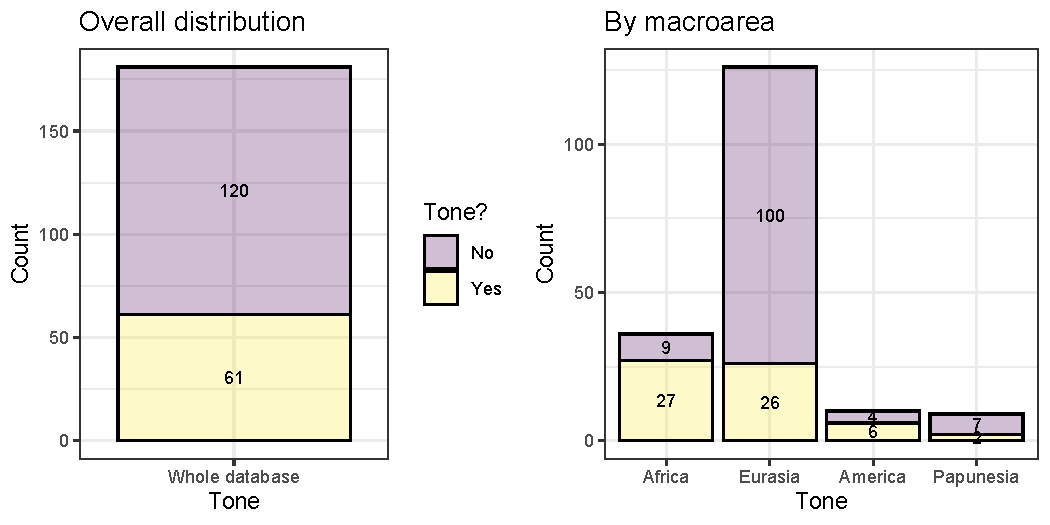
\includegraphics[width=\textwidth]{../../code/figures/tone1_distribution}
  \caption{Distribution (as number of languages) of \textit{tone1} (no tone vs any type of tone system) across the full database (left) and by macroarea (right). Please note that the vertical axes have different scales to avoid the macroareas with small sample sizes to be visually ``squashed'' by the whole database.}
  \label{Fig:tone1_distribution}
\end{figure}

The relationship between \textit{tone1} and the population frequency of the two ``derived'' alleles is shown in Figure \ref{Fig:tone1_alleles}.
It can seen that, globally, there seems to be a difference between languages with and without tone: while tone languages (\textit{tone1} == ``Yes'') tend to be found when \textit{ASPM}-D has a low frequency, the others (\textit{tone1} == ``No'') tend to be found at high frequencies of both ``derived'' alleles.
Zooming in on each macroarea shows different patterns: while there seems to be a difference for \textit{ASPM}-D in Eurasia (higher for ``No'') and Papunesia (lower for ``No''), there seems to be no differences in Africa and America.
However, such plots can be very misleading because these points represent related languages and/or alternative genetic and linguistics values for the same sample -- actual statistical analyses are needed.

\begin{figure}[h]
  \centering
  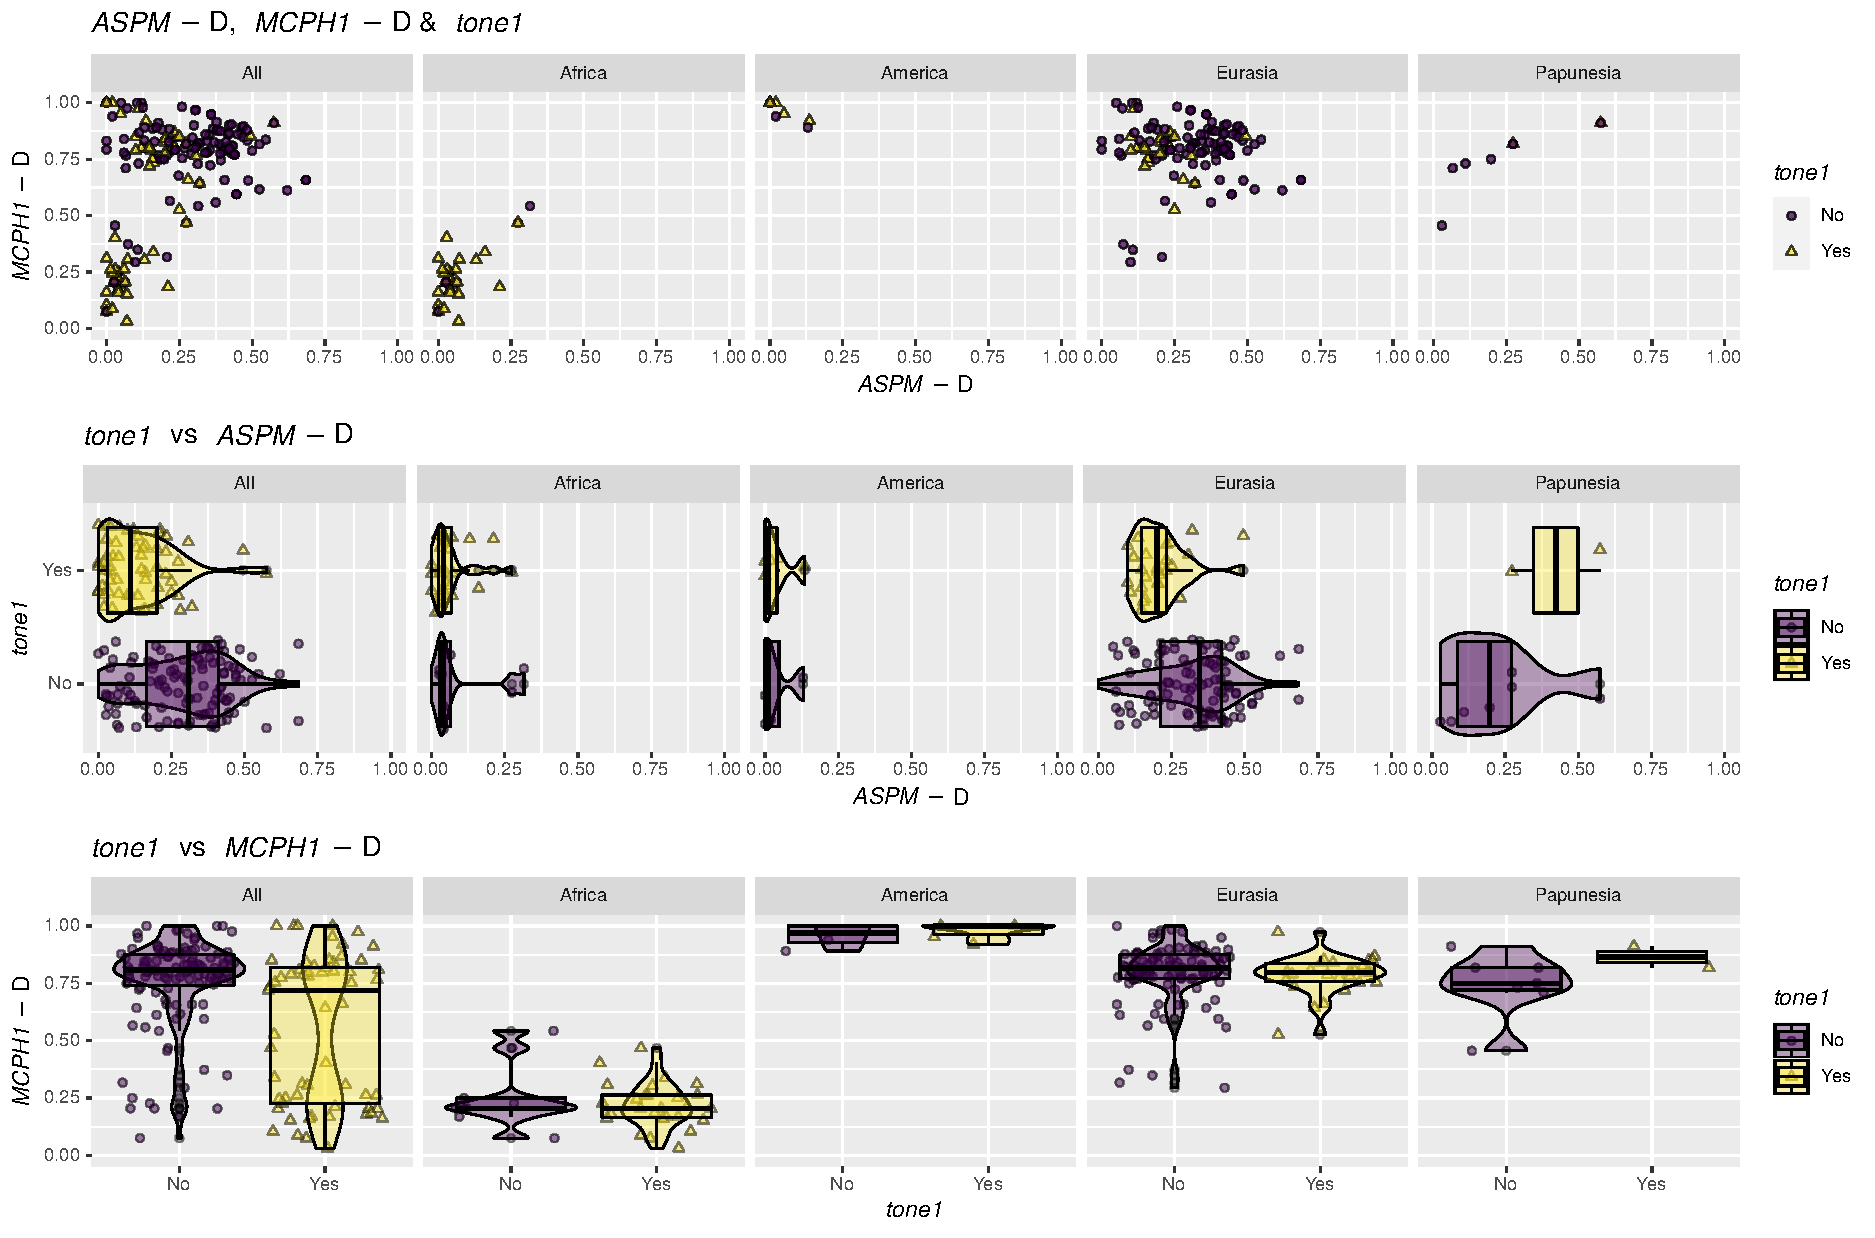
\includegraphics[width=\textwidth]{../../code/figures/tone1_alleles}
  \caption{Relationship between tone1 (colour \& shape) and the population frequency of \textit{ASPM}-D and \textit{MCPH1}-D in the whole database and separately by macroarea (columns). Top row: scatter plots of \textit{ASPM}-D (horizontal axis) and \textit{MCPH1}-D (vertical axis) versus \textit{tone1} (dot colour \& shape). Next two rows show the ``derived'' allele frequency (as actual jittered observations, violin plots and boxplots) versus \textit{tone1} values (color) for \textit{ASPM}-D (middle row) and \textit{MCPH1}-D (bottom row); please note that the orientation of the axis showing the ``derived'' allele frequency is the same as in the top row plots (i.e., x-axis for \textit{ASPM}-D, and y-axis for \textit{MCPH1}-D.}
  \label{Fig:tone1_alleles}
\end{figure}


\paragraph{Regressions}

I fitted a mixed-effects logistic regression model of \textit{tone1} on \textit{macroarea}, the population frequencies of the two ``derived'' alleles and all their pairwise interactions as fixed effects, and \textit{family} as random effect\footnote{Building on the notations in footnote \ref{note_reg_R}: $t1 \sim 1 + a + m +  M + a:M + m:M + a:m + (1 \mid F)$, where $t1$ is \textit{tone1}, and $:$ represents interactions.} to the whole data.
First, as expected, \textit{tone1} is strongly clustered within families ($ICC(tone1) = 71.1\%$).
Second, the interactions do not contribute (\textit{p}(\textit{ASPM}-D:\textit{MCPH}-D) = 0.27, \textit{p}(\textit{ASPM}-D:\textit{macroarea} + \textit{MCPH}-D:\textit{macroarea}) = 0.19)\footnote{Such $p$-values result from comparing the model with the predictor(s) and/or interaction(s) of interest, against the identical model but with them removed, using an appropriate test as implemented by \texttt{R}'s \texttt{anova()} function (here, for logistic regressions, a $\chi^2$ test).} and were removed from the model.
Third, as expected, \textit{macroarea} predicts \textit{tone1} by itself ($p = 0.00082$, $R^2 = 23.3\%$\footnote{For mixed-effects models, the proportion of variance explained by the model is represented by \emph{Nakagawa's} $R^2$, where the \emph{marginal} estimate considers only the fixed effects, while the \emph{conditional} also considers the random effects as well. Here, I only show the marginal $R^2$, as we are interested in the fixed effects.}).
Fourth, when excluding \textit{macroarea} from the model, the two ``derived'' alleles together predict tone ($p = 0.0049$, $R^2 = 13.4\%$), with each by itself having negative significant effects on \textit{tone1} (\textit{ASPM}-D: $\beta = -6.0 \pm 2.2$, $p = 0.0041$, $R^2 = 10.0\%$; \textit{MCPH1}-D $\beta = -4.0 \pm 1.5$, $p = 0.0064$, $R^2 = 9.4\%$).
However, adding \textit{macroarea} as a fixed effect makes the specific contributions of the two ``derived'' alleles not significant (\textit{ASPM}-D: $\beta = -2.2 \pm 2.7$, $p = 0.41$; \textit{MCPH1}-D: $\beta = -1.5 \pm 2.2$, $p = 0.49$).

Conducting separate regressions in Africa and Eurasia (as they have enough data; also removing \textit{macroarea} as a fixed effect), finds a negative effect of \textit{ASPM}-D in both (Africa: $\beta = -25.9 \pm 20.7$, $p = 0.035$; Eurasia: $\beta = -6.7 \pm 1.9$, $p = 0.00011$), but only when not modelling language family.
Please note that for Africa there is almost no variation between families to allow its inclusion as a random effect, and, when included as fixed effect, family does not contribute significantly ($p = 0.41$).
For Eurasia, family can be included as a random or as a fixed effect, and when doing so, the partial effect of \textit{ASPM}-D becomes not significant (as random effect: $\beta = 0.7 \pm 3.9$, $p = 0.86$; as fixed effect: $\beta = 1.6 \pm 4.1$, $p = 0.7$).

Permuting\footnote{Because permutations and restricted sampling involve random sampling, the results might differ slightly between runs.} (with or without restrictions) the observations, shows that \textit{ASPM}-D has a negative effect on \textit{tone1}, especially clear when not controlling for \textit{macroarea}, but still present when including it as a fixed effect (except when restricting the permutations within families, which is not surprising given the strong clustering within families of both \textit{ASPM}-D and \textit{tone1}).
In contrast, for \textit{MCPH1}-D, there is a negative effect only for unrestricted permutations when not controlling for \textit{macroarea}.
Please see Figure \ref{Fig:tone1_regressions_permuted}.

\begin{figure}[h]
  \centering
  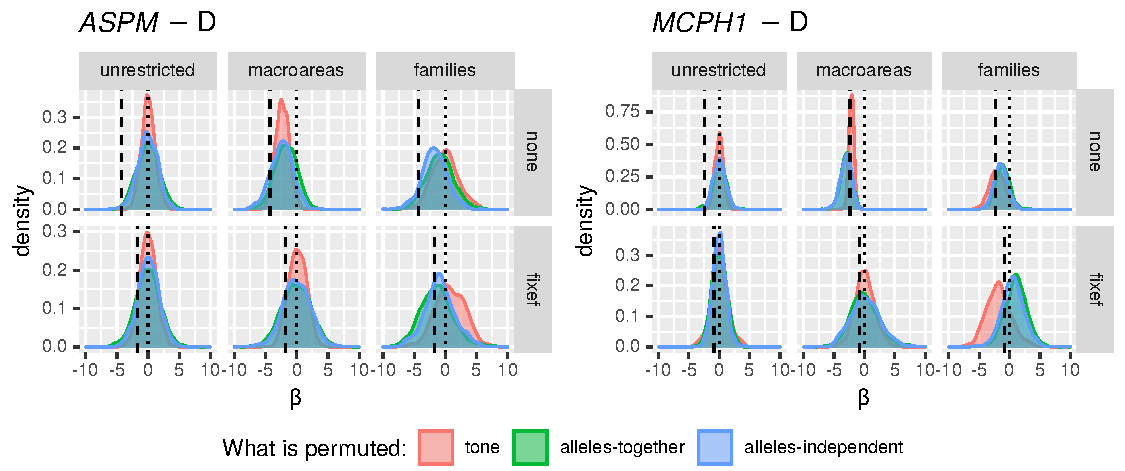
\includegraphics[width=\textwidth]{../../code/figures/tone1_regressions_permuted}
  \caption{Distribution of the effect size $\beta$ (horizontal axis) of \textit{ASPM}-D (left) and \textit{MCPH1}-D (right) on \textit{tone1} in the permutation regressions without restrictions (``unrestricted''), only within macroareas (``macroareas''), and only within families (``families''), without controlling for macroarea (``none'') or when including macroarea as a fixed effect (``fixef''). Each individual plot shows the original $\beta$ obtained on the unpermuted data (vertical dashed black line), 0.0 (vertical dotted black thin line), and the distribution of the permuted $\beta$ for the three variables to be permuted (the coloured areas): tone by itself (red), the two ``derived'' alleles together as a unit (green), and the two ``derived'' alleles shuffled individually (blue). Please note that the y-axes vary between plots, but the x-axes are fixed between -10.0 and 10.0 for comparability. If a distribution is centred on 0.0 (e.g., ``ASPM''/``unrestricted''/``none'' in the top left) then the permuted data show no effect of the ``derived'' allele (here, \textit{ASPM}-D) on tone (i.e., the regression slope $\beta$ is 0.0). The less overlap is between the observed $\beta$ (dashed black line) and such a distribution, the more ``special'' the relationship between the ``derived'' allele and tone is relative to the structure destroyed by that specific permutation; conversely, if the observed $\beta$ is largely included in a distribution, the more such a value is expected by chance given the constraints of the permutation.}
  \label{Fig:tone1_regressions_permuted}
\end{figure}

Repeated restricted sampling, where only one sample is randomly chosen per family, also shows a clear negative effect of \textit{ASPM}-D on \textit{tone1} even when controlling for \textit{macroarea} and \textit{MCPH1}-D ($\approx 83\%$ of the $\beta$'s < 0, with a mean $\overline{\beta} \approx -2.6$), and a weaker but still discernible one for \textit{MCPH1}-D even when controlling for \textit{macroarea} and \textit{ASPM}-D ($\approx 69\%$ of the $\beta$'s < 0, with a mean $\overline{\beta} \approx -1.5$); see Figure \ref{Fig:tone1_regressions_restricted}.

\begin{figure}[h]
  \centering
  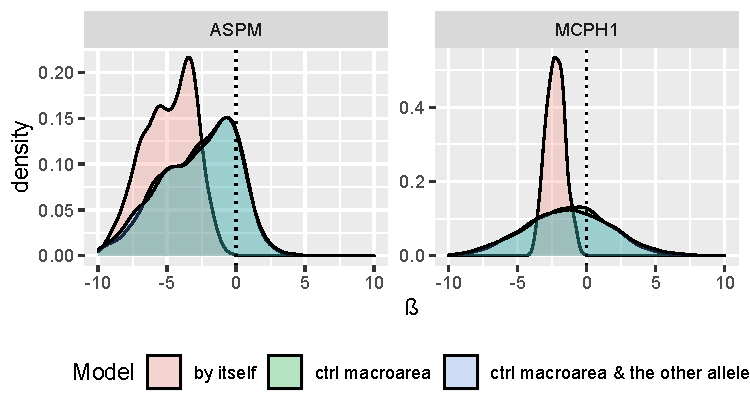
\includegraphics[width=0.6\textwidth]{../../code/figures/tone1_regressions_restricted}
  \caption{Distribution of the effect size $\beta$ (horizontal axis) of \textit{ASPM}-D (left) and \textit{MCPH1}-D (right) on \textit{tone1} in the restricted sampling regressions without controlling for macroareas (``by itself'', red areas), including macroarea as a fixed effect (``ctrl macroarea'', green areas), and including both macroarea and the other ``derived'' allele as fixed effects (``ctrl macroarea \& the other allele'', blue areas). Each individual plot shows 0.0 (vertical dotted black thin line) and the distribution of the $\beta$'s for the three ``models'' (the coloured areas). Please note that the y-axes vary between plots, but the x-axes are fixed between -10.0 and 10.0 for comparability. The more to the left of 0.0 a distribution is, the clearer the negative effect is.}
  \label{Fig:tone1_regressions_restricted}
\end{figure}


\paragraph{Mediation analysis}

I ran two separate mediation analyses (see Figure \ref{Fig:mediation_analysis}) with the treatment (\textit{IV}) = \textit{dichotomised macroarea} (Africa vs the rest of the world), the outcome (\textit{DV}) = \textit{tone1}, and the \textit{mediator} (\textit{MV}) = either \textit{ASPM}-D or \textit{MCPH1}-D, respectively.

Using the full dataset, both models find a significant positive \textit{total effect} ($TE$) of macroarea on tone (\textit{ASPM}-D: $0.50$, 95\%CI $(0.33, 0.64)$, $p < 2\cdot10^{-16}$; \textit{MCPH1}-D:  $0.50$, 95\%CI $(0.33, 0.65)$, $p < 2\cdot10^{-16}$), confirming that African languages tend to be more tonal in our database than languages outside Africa, as well as a significant positive \textit{average direct effect} ($ADE$; coefficient $c'$ in Figure \ref{Fig:mediation_analysis}) of \textit{macroarea} on \textit{tone1} (\textit{ASPM}-D: $0.28$, 95\%CI $(0.08, 0.48)$, $p = 0.002$; \textit{MCPH1}-D:  $0.54$, 95\%CI $(0.19, 0.76)$, $p = 0.008$).
However, the average \textit{indirect effects} ($ACME$), mediated by the ``derived'' allele frequencies, differ strongly between them: for \textit{ASPM}-D, the mediated effect is significant and positive ($0.21$, 95\%CI $(0.10, 0.32)$, $p = 0.002$), representing 42.8\% of the total effect and resulting from a significant negative effect of being in Africa on \textit{ASPM}-D (coefficient $a$; $-0.21 \pm0.03$, $p = 7.7\cdot10^{-13}$), and a significant negative effect of \textit{ASPM}-D on tone (coefficient $b$; $-5.40 \pm1.42$, $p = 0.00015$).
For \textit{MCPH1}-D, the mediated effect is not significant ($-0.04$, 95\%CI $(-0.22, 0.24)$, $p = 0.6$), composed of a significant negative effect of being in Africa on \textit{MCPH1}-D (coefficient $a$; $-0.57 \pm0.02$, $p = 9.9\cdot10^{-59}$), and a non-significant effect of \textit{MCPH1}-D on tone (coefficient $b$; $0.75 \pm1.44$, $p = 0.6$).
Taken together, this shows that there's a positive effect of being in Africa on tone, but that about half of it is mediated by the negative effect of \textit{ASPM}-D, but not by \textit{MCPH1}-D; moreover, the frequency of \textit{MCPH1}-D is shaped much more by being in or outside Africa than that of \textit{ASPM}-D.

Restricted sampling (repeated 1,000 times) finds the same pattern (see Figure \ref{Fig:tone1_mediation_restricted} and Table \ref{Tab:tone1_mediation_restricted}), with only \textit{ASPM}-D mediating part of the influence of macroarea on tone, but not \textit{MCPH1}-D; also, macroarea has a much stronger effect the latter.
This procedure does control for language family, but, on the other hand, drastically reduces the sample size to only $N=35$ unique families, resulting in a low power of the individual mediation analyses, with relatively few effect sizes being large enough for statistical significance, but even so, there are many more significant indirect effects for \textit{ASPM}-D (9.2\% at $\alpha$-level 0.05, and 27.9\% at $\alpha$-level 0.10) than for \textit{MCPH1}-D (0.1\% and 1.1\%, respectively).

\begin{figure}[h]
  \centering
  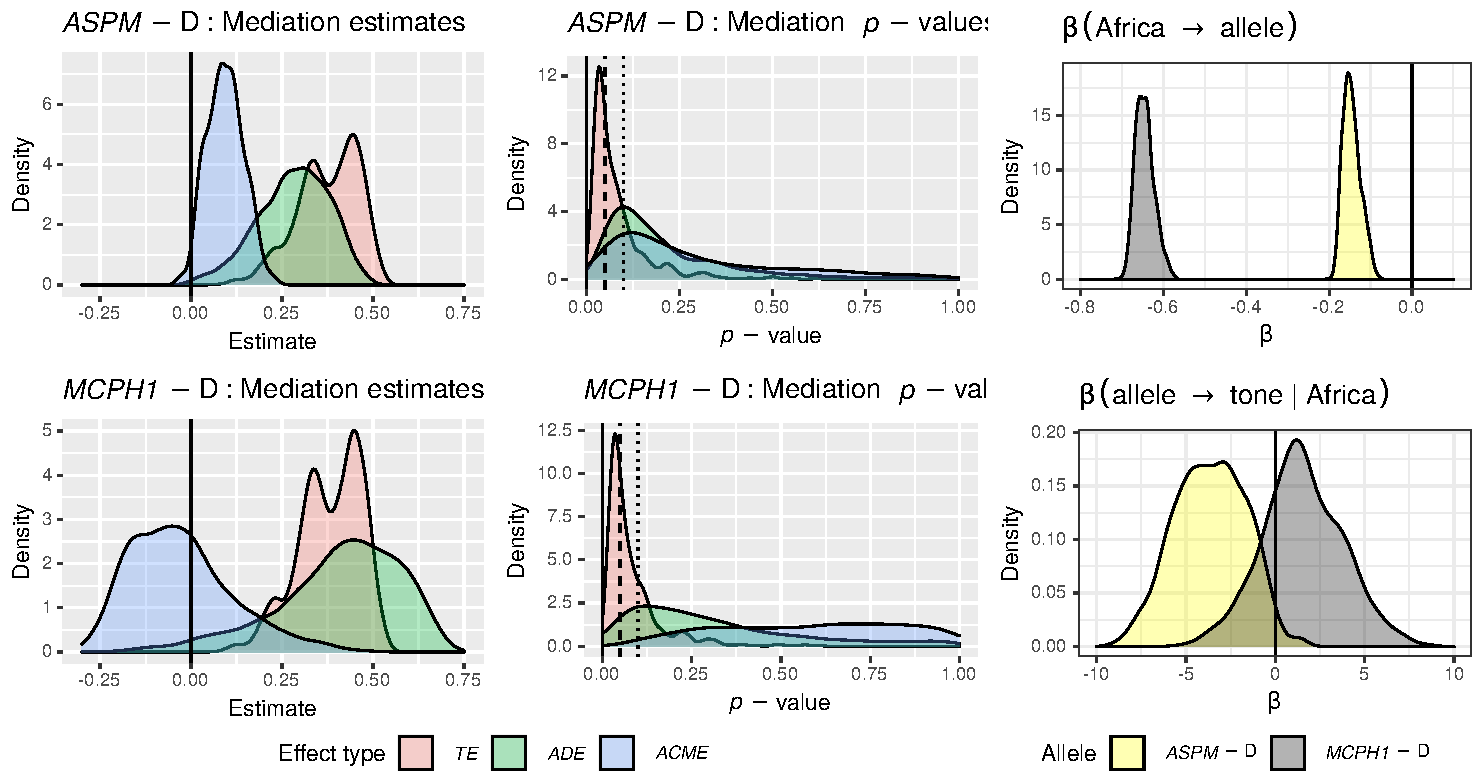
\includegraphics[width=\textwidth]{../../code/figures/tone1_mediation_restricted}
  \caption{Mediation analysis for 1,000 restricted samples for \textit{tone1}. The leftmost two panels show the distribution of point estimates (coloured areas) of the \textit{Total Effect} ($TE$), the \textit{Direct Effect} ($AD$E) and the \textit{Indirect Effect} ($ACM$E) for \textit{ASPM}-D and \textit{MCHP1}-D; the middle two panels show the distribution of the \textit{p}-values (coloured areas) for the same effects, while the two rightmost panels (on white background) show the distribution of the regression slopes ($\beta$) for the two alleles (top: for the regression of the allele frequency on being within or outside Africa, and bottom: for the regression of tone on the allele while controlling for being within or outside Africa). The black vertical lines are: 0.0 (solid), 0.05 (dashed) and 0.10 (dotted). Please note that the y-axes vary between plots, but the x-axes of the four left panels (but not of the two right panels) are fixed for comparability. Mediation estimates (leftmost panels): $ACME$ (blue) should be away from 0 for a sizeable mediation through the ``derived'' allele. Mediation \textit{p}-values (mid panels): $ACME$ (blue) should be below 0.05 (or 0.10) for a statistically significant mediation through the ``derived'' allele. (Partial) regression slopes $\beta$ (rightmost panels): should be different from 0. See Table \ref{Tab:tone1_mediation_restricted} for the numeric summaries.}
  \label{Fig:tone1_mediation_restricted}
\end{figure}

\begin{table}[h]
  \caption{Summaries of the mediation analysis for 1,000 restricted samples for \textit{tone1}. For each ``derived'' allele the table shows the three types of effects (total, direct and mediated) and the two (partial) regression coefficients. For each, it gives the mean, median and the results of the relevant comparison with 0.0 (smaller or bigger) in terms of the percent of the estimates smaller (or bigger) than 0.0 and the one-sided \textit{t}-test; the direction of the comparison is based on \textit{a priori} expectancies: positive effects but negative $\beta$s.}
  \label{Tab:tone1_mediation_restricted}
  \centering
  \begin{tabular}{|l|l|r|r|l|}
    \toprule
    \textbf{Allele} & \textbf{Estimate} & \textbf{Mean} & \textbf{Median} & \textbf{Compared to 0} \\
    \midrule
    \multirow{5}{*}{\textit{ASPM}-D} & $TE$ & 0.38 & 0.38 & > 0: 100.0\%, $t = 141.1$, $p < 2.2\cdot10^{-16}$ \\
      & $ADE$ & 0.28 & 0.29 & > 0: 99.8\%, $t = 91.9$, $p < 2.2\cdot10^{-16}$ \\
      & $ACME$ & 0.094 & 0.093 & > 0: 98.3\%, $t = 59.5$, $p < 2.2\cdot10^{-16}$ \\
      & $\beta$(Africa $\rightarrow$ allele) & -0.15 & -0.15 & < 0: 100.0\%, $t = -216.9$, $p < 2.2\cdot10^{-16}$ \\
      & $\beta$(allele $\rightarrow$ tone $\mid$ Africa) & -3.6 & -3.6 & < 0: 98.0\%, $t = -58.0$, $p < 2.2\cdot10^{-16}$ \\
    \midrule
    \multirow{5}{*}{\textit{MCPH1}-D} & $TE$ & 0.38 & 0.39 & > 0: 100.0\%, $t = 140.6$, $p < 2.2\cdot10^{-16}$ \\
      & $ADE$ & 0.41 & 0.43 & > 0: 97.6\%, $t = 76.5$, $p < 2.2\cdot10^{-16}$ \\
      & $ACME$ & -0.027 & -0.045 & > 0: 36.9\%, $t = -6.0$, $p = 1$ \\
      & $\beta$(Africa $\rightarrow$ allele) & -0.65 & -0.65 & < 0: 100.0\%, $t = -899.4$, $p < 2.2\cdot10^{-16}$ \\
      & $\beta$(allele $\rightarrow$ tone $\mid$ Africa) & 1.5 & 1.4 & < 0: 24.2\%, $t = 21.4$, $p = 1$ \\
    \bottomrule
  \end{tabular}
\end{table}


\paragraph{Path analysis}

I ran path analyses (see Figure \ref{Fig:path_analysis}) with the treatment (\textit{IV}) = \textit{dichotomised macroarea} (Africa vs the rest of the world), the outcome (\textit{DV}) = \textit{tone1}, and the \textit{mediators} \textit{MV}\textsubscript{1} = \textit{ASPM}-D and \textit{MV}\textsubscript{2} = \textit{MCPH1}-D, separately for the binary and the ordered codings of the \textit{IV} and the \textit{DV} (but given that the results are extremely similar, I only report here the numeric coding).

Using the full dataset, the model fits the data very well ($\chi^2_{1} = 0.22$, $p = 0.22$; $CFI=1.00$, $TLI=1.01$, $NNFI=1.01$ and $RFI=1.00$)\footnote{Please note that, for path analyses/SEM models, we want the $\chi^2$ goodness-of-fit test to be \emph{not} significant, meaning that there is no reason to reject the hypothesis that the model fits the data; this is a binary decision. On the other hand, there are several \emph{fit indices} (I only show a few: $CFI$, $TLI$, $NNFI$ and $RFI$), which are continuous, the closer to $1.00$, the better the model fits to the data.}, and, as shown in Figure \ref{Fig:tone1_path_all}, being in Africa has a significant positive direct effect on \textit{tone1}, a significant negative effect on \textit{ASPM}-D which has a negative significant effect on \textit{tone1}, but while it has a stronger significant negative effect on \textit{MCHP1}-D this has no effect on \textit{tone1}.

\begin{figure}[h]
  \centering

  \begin{tikzpicture}[node distance=4.0cm]
  \node(iv) {\textit{Africa}};
  \node(dv)[right of=iv] {\textit{tone1}};
  \node(m1)[above of=dv] {\textit{ASPM}-D};
  \node(m2)[below of=dv] {\textit{MCPH1}-D};
  \draw[->, very thick, red] (iv) -- (dv) node[midway, above] {0.33 (0.019)};
  \draw[->, very thick, blue] (iv) -- (m1) node[midway, left] {-0.50 (0.000)};
  \draw[->, very thick, blue] (m1) -- (dv) node[midway, right] {-0.30 (0.000)};
  \draw[->, very thick, blue] (iv) -- (m2) node[midway, left] {-0.88 (0.000)};
  \draw[->, thin, gray, dotted] (m2) -- (dv) node[midway, right] {0.05 (0.68)};
  \end{tikzpicture}

  \caption{The path model for \textit{tone1} fitted on all the data, showing the standardized path coefficients (and their \textit{p}-values in parentheses); gray dotted = not significant, red = significant positive, and blue = significant negative. }
  \label{Fig:tone1_path_all}
\end{figure}

As for the mediation analysis above, restricted sampling finds a similar pattern (see Figure \ref{Fig:tone1_path_restricted} and Table \ref{Tab:tone1_path_restricted}).

\begin{figure}[h]
  \centering

  \begin{tikzpicture}[node distance=4.0cm]
  \node(iv) {\textit{Africa}};
  \node(dv)[right of=iv] {\textit{tone1}};
  \node(m1)[above of=dv] {\textit{ASPM}-D};
  \node(m2)[below of=dv] {\textit{MCPH1}-D};
  \draw[->, thin, red] (iv) -- (dv) node[midway, above] {0.41 (0.48)};
  \draw[->, very thick, blue] (iv) -- (m1) node[midway, left] {-0.15 (0.03)};
  \draw[->, thin, blue] (m1) -- (dv) node[midway, right] {-0.69 (0.52)};
  \draw[->, very thick, blue] (iv) -- (m2) node[midway, left] {-0.65 (0.03)};
  \draw[->, thin, gray, dotted] (m2) -- (dv) node[midway, right] {0.14 (0.63)};
  \end{tikzpicture}

  \caption{Summary of the 1,000 path models for \textit{tone1} fitted to restricted samples, showing the medians of the standardized path coefficients (and their IQR, in parentheses); conventions as in Figure \ref{Fig:tone1_path_all}. }
  \label{Fig:tone1_path_restricted}
\end{figure}

\begin{table}[h]
  \caption{Summaries of the path analysis for 1,000 restricted samples for \textit{tone1}. Similar conventions as for Table \ref{Tab:tone1_mediation_restricted}.}
  \label{Tab:tone1_path_restricted}
  \centering
  \begin{tabular}{|l|l|r|r|l|}
    \toprule
    \textbf{Type} & \textbf{Estimate} & \textbf{Mean (SD)} & \textbf{Median (IQR)} & \textbf{Compared to 0} \\
    \midrule
    \multirow{5}{*}{Fit} & $\chi^2$ test & 95.3\% n.s. & - & - \\
    & $CFI$              & 0.99 (0.01) & 1.00 (0.01) & - \\
    & $TLI$              & 0.98 (0.10) & 1.00 (0.15) & - \\
    & $NNFI$             & 0.98 (0.10) & 1.00 (0.15) & - \\
    & $RFI$              & 0.90 (0.09) & 0.93 (0.13) & - \\
    \midrule
    \multirow{4}{*}{Path} & Africa $\rightarrow$ \textit{tone1} &  0.41 (0.33) &  0.41 (0.48) & 88.8\%  > 0 \\
    & Africa $\rightarrow$ \textit{ASPM}-D                      & -0.15 (0.02) & -0.15 (0.03) & 100.0\% < 0 \\
    & \textit{ASPM}-D  $\rightarrow$ \textit{tone1}             & -0.70 (0.35) & -0.69 (0.52) & 98.7\%  < 0 \\
    & Africa $\rightarrow$ \textit{MCPH1}-D                     & -0.64 (0.02) & -0.65 (0.03) & 100.0\% < 0 \\
    & \textit{MCPH1}-D $\rightarrow$ \textit{tone1}             &  0.13 (0.44) &  0.14 (0.63) & 37.7\%  < 0 \\
    \bottomrule
  \end{tabular}
\end{table}


\paragraph{Decision trees}

If, besides \textit{ASPM}-D and \textit{MCHP1}-D, \textit{macroarea} is also included, the decision tree fits the full dataset well (accuracy = 77.3\%, sensitivity = 71.7\%, specificity = 79.3\%, precision = 54.1\%, and recall = 71.7\%), and generalises across 100 training/testing sets (mean $\pm$ sd: accuracy = 75.3\% $\pm$6.4\%, sensitivity = 70.0\% $\pm$14.6\%, specificity = 77.4\% $\pm$6.3\%, precision = 49.4\% $\pm$11.9\%, recall = 70.0\% $\pm$14.6\%), and suggests that within Eurasia and Papunesia, the frequency of \textit{ASPM}-D is a good predictor of \textit{tone1} (with $p = 0.002$).
When \textit{macroarea} is not included, then the fit for the whole dataset drops a bit (accuracy = 75.1\%, sensitivity = 75.0\%, specificity = 75.2\%, precision = 39.3\%, and recall = 75.0\%) and generalises slightly less well (accuracy = 69.9\% $\pm$6.2\%, sensitivity = 59.6\% $\pm$18.5\%, specificity = 74.1\% $\pm$7.0\%, precision = 39.8\% $\pm$18.9\%, recall = 59.6\% $\pm$18.5\%); now, \textit{ASPM}-D is predictive overall ($p < 0.001$), and \textit{MCPH1}-D is relevant ($p = 0.004$) only for low frequencies of \textit{ASPM}-D (see Figure \ref{Fig:tone1_decision_trees}).

\begin{figure}[h]
  \centering
  \begin{subfigure}{0.75\linewidth}
    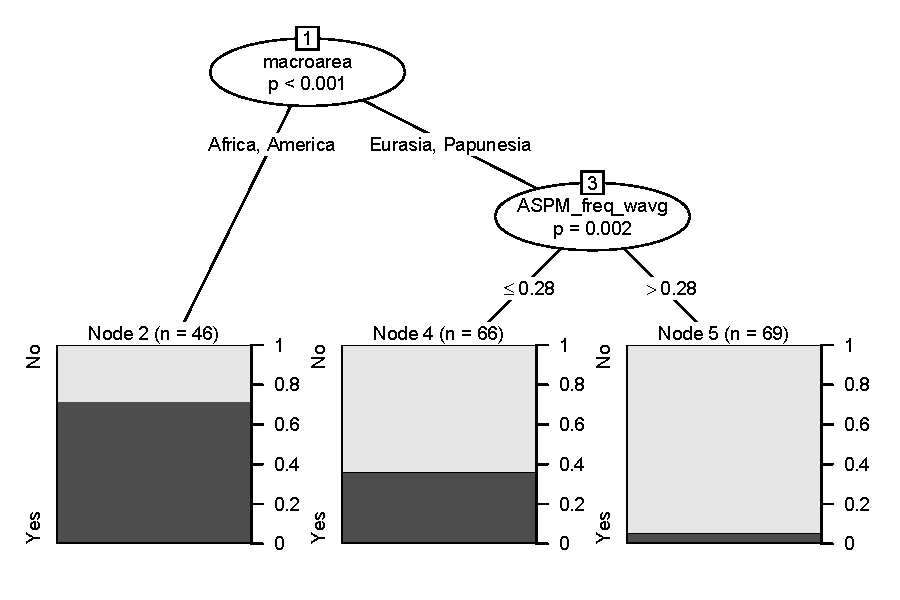
\includegraphics[width=\textwidth]{../../code/figures/tone1_decision_trees_macroarea}
  \end{subfigure}
  \begin{subfigure}{0.75\linewidth}
    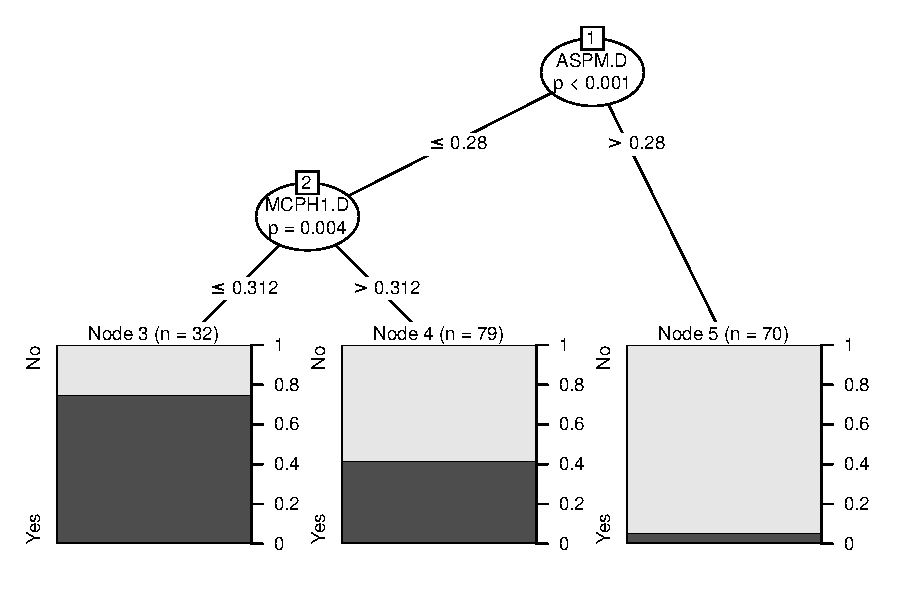
\includegraphics[width=\textwidth]{../../code/figures/tone1_decision_trees_nomacroarea}
  \end{subfigure}
  \caption{Decision trees for \textit{tone1} including \textit{macroarea} as a predictor (top) or not (bottom). Please note that in these decision tree plots ``ASPM.D'' and ``MCPH1.D'' stand for \textit{ASPM}-D and \textit{MCPH1}-D, respectively. Each split is a binary decision based on the values or conditions on the branches (with the $p$-value in parentheses). The bars at the bottom of the plots show the distribution of ``No'' (light gray') and ``Yes'' (dark gray) values and the number of observations for that case (e.g., $n = 69$ in the top panel's rightmost bar, means that 69 observations are in Eurasia and Papunesia with the population frequency of \textit{ASPM}-D > 0.28, and for those only a minority of $\approx 6\%$ have tone). It can be seen that in the bottom panel, a low frequency of \textit{MCPH1}-D seems to be a proxy for Africa.}
  \label{Fig:tone1_decision_trees}
\end{figure}


\paragraph{Random forests}

If \textit{macroarea} is included as a predictor, the random forests fit the data well (accuracy = 77.8\% $\pm$0.9\%, sensitivity = 68.9\% $\pm$1.8\%, specificity = 81.6\% $\pm$0.4\%, precision = 62.\% $\pm$1.0\%, recall = 68.9\% $\pm$1.8\%), and the conditional random forests are even better (accuracy = 84.5\% $\pm$0.6\%, sensitivity = 78.9\% $\pm$0.4\%, specificity = 87.0\% $\pm$0.7\%, precision = 73.5\% $\pm$1.7\%, recall = 78.9\% $\pm$0.4\%).
Of the 3 measures of variable importance, the mean decrease in accuracy for the random forests finds that \textit{macroarea} > \textit{ASPM}-D > \textit{MCPH1}-D, the mean decrease in node impurity for the random forests finds that \textit{ASPM}-D > \textit{MCPH1}-D > \textit{macroarea}, and the unconditional importance for the conditional random forests finds that \textit{ASPM}-D > \textit{macroarea} > \textit{MCPH1}-D.

Leaving macroarea out slightly reduces the fit (random forests: accuracy = 70.6\% $\pm$1.0\%, sensitivity = 56.1\% $\pm$1.4\%, specificity = 78.5\% $\pm$0.8\%, precision = 58.6\% $\pm$1.9\%, recall = 56.1\% $\pm$1.4\%; conditional random forests: accuracy = 82.1\% $\pm$0.5\%, sensitivity = 81.6\% $\pm$0.9\%, specificity = 82.3\% $\pm$0.5\%, precision = 60.6\% $\pm$1.3\%, recall = 81.6\% $\pm$0.9\%), but now all three criteria agree that \textit{ASPM}-D > \textit{MCPH1}-D.


\paragraph{Conclusions}

Thus, for \textit{tone1}, capturing the presence of any type of tone system, \textit{macroarea} (and especially being or not in Africa) shapes simultaneously the distribution of tone and of the two ``derived'' alleles.
This makes it very hard to disentangle the direct influence of macroarea on tone (as a proxy for linguistic and genetic processes) from any indirect effects mediated by the two ``derived'' alleles.
Nevertheless, the overarching pattern is that the two ``derived'' alleles by themselves have a negative effect on tone even when controlling for family, but this largely overlaps with the effect of macroarea (especially Africa vs the rest of the world), fully explaining the influence of \textit{MCPH1}-D.
In contrast, there seems to be a negative effect of \textit{ASPM}-D on tone above and beyond the influence of macroarea and family.




\subsection{Is there complex tone? (\textit{tone2})}

While the original hypothesis in \citet{dediu_ladd_2007} concerns strictly the presence of tone, here I capitalise on the availability of data allowing the comparison of languages with a complex tone system versus those without tone or with a simple system -- this is embodied in the \textit{tone2} variable, where ``Yes'' represents complex tone systems.

When selecting all unique observations with non-missing data for \textit{tone2}, \textit{ASPM}-D and \textit{MCPH1}-D, there are 165 observations, distributed among 108 unique Glottolg codes (languages) in 35 families (the number of languages per family ranges from 1 to 44, with mean 4.7 and median 2).
There are 25 (15.2\%) languages with complex tone (``Yes'') in the dataset ($\chi^2_{1} = 80.2$, $p < 2.2\cdot10^{-16}$), and the distribution by macroarea is 30 (7 = 23.3\% ``Yes'') in Africa, 115 (16 = 13.9\%) in Eurasia, 10 (1 = 10\%) in America, and 10 (1 = 10\%) in Papunesia (between macroareas $\chi^2_{3} = 2.1$, $p = 0.55$); see Figure \ref{Fig:tone2_distribution}.

\begin{figure}[h]
  \centering
  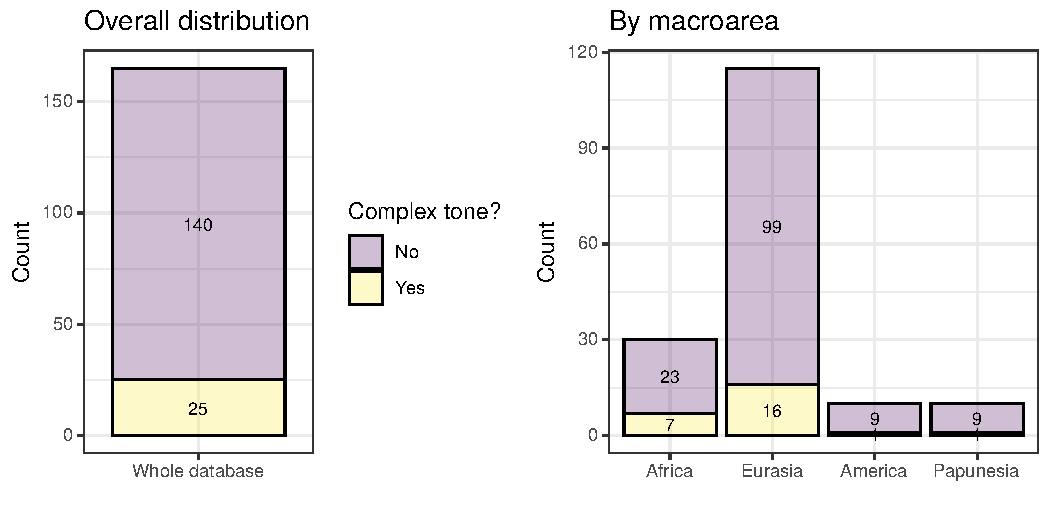
\includegraphics[width=\textwidth]{../../code/figures/tone2_distribution}
  \caption{Distribution (as counts) of \textit{tone2} (no and simple tone vs complex tone) across the full database (left) and by macroarea (right). Same conventions as in Figure \ref{Fig:tone1_distribution}.}
  \label{Fig:tone2_distribution}
\end{figure}

The relationship between \textit{tone2} and the population frequency of the two ``derived'' alleles is shown in Figure \ref{Fig:tone2_alleles}.
It can seen that, globally, it seems that languages with complex tone tend to be found when \textit{ASPM}-D has a low frequency, which seems to be the case also in Eurasia.

\begin{figure}[h]
  \centering
  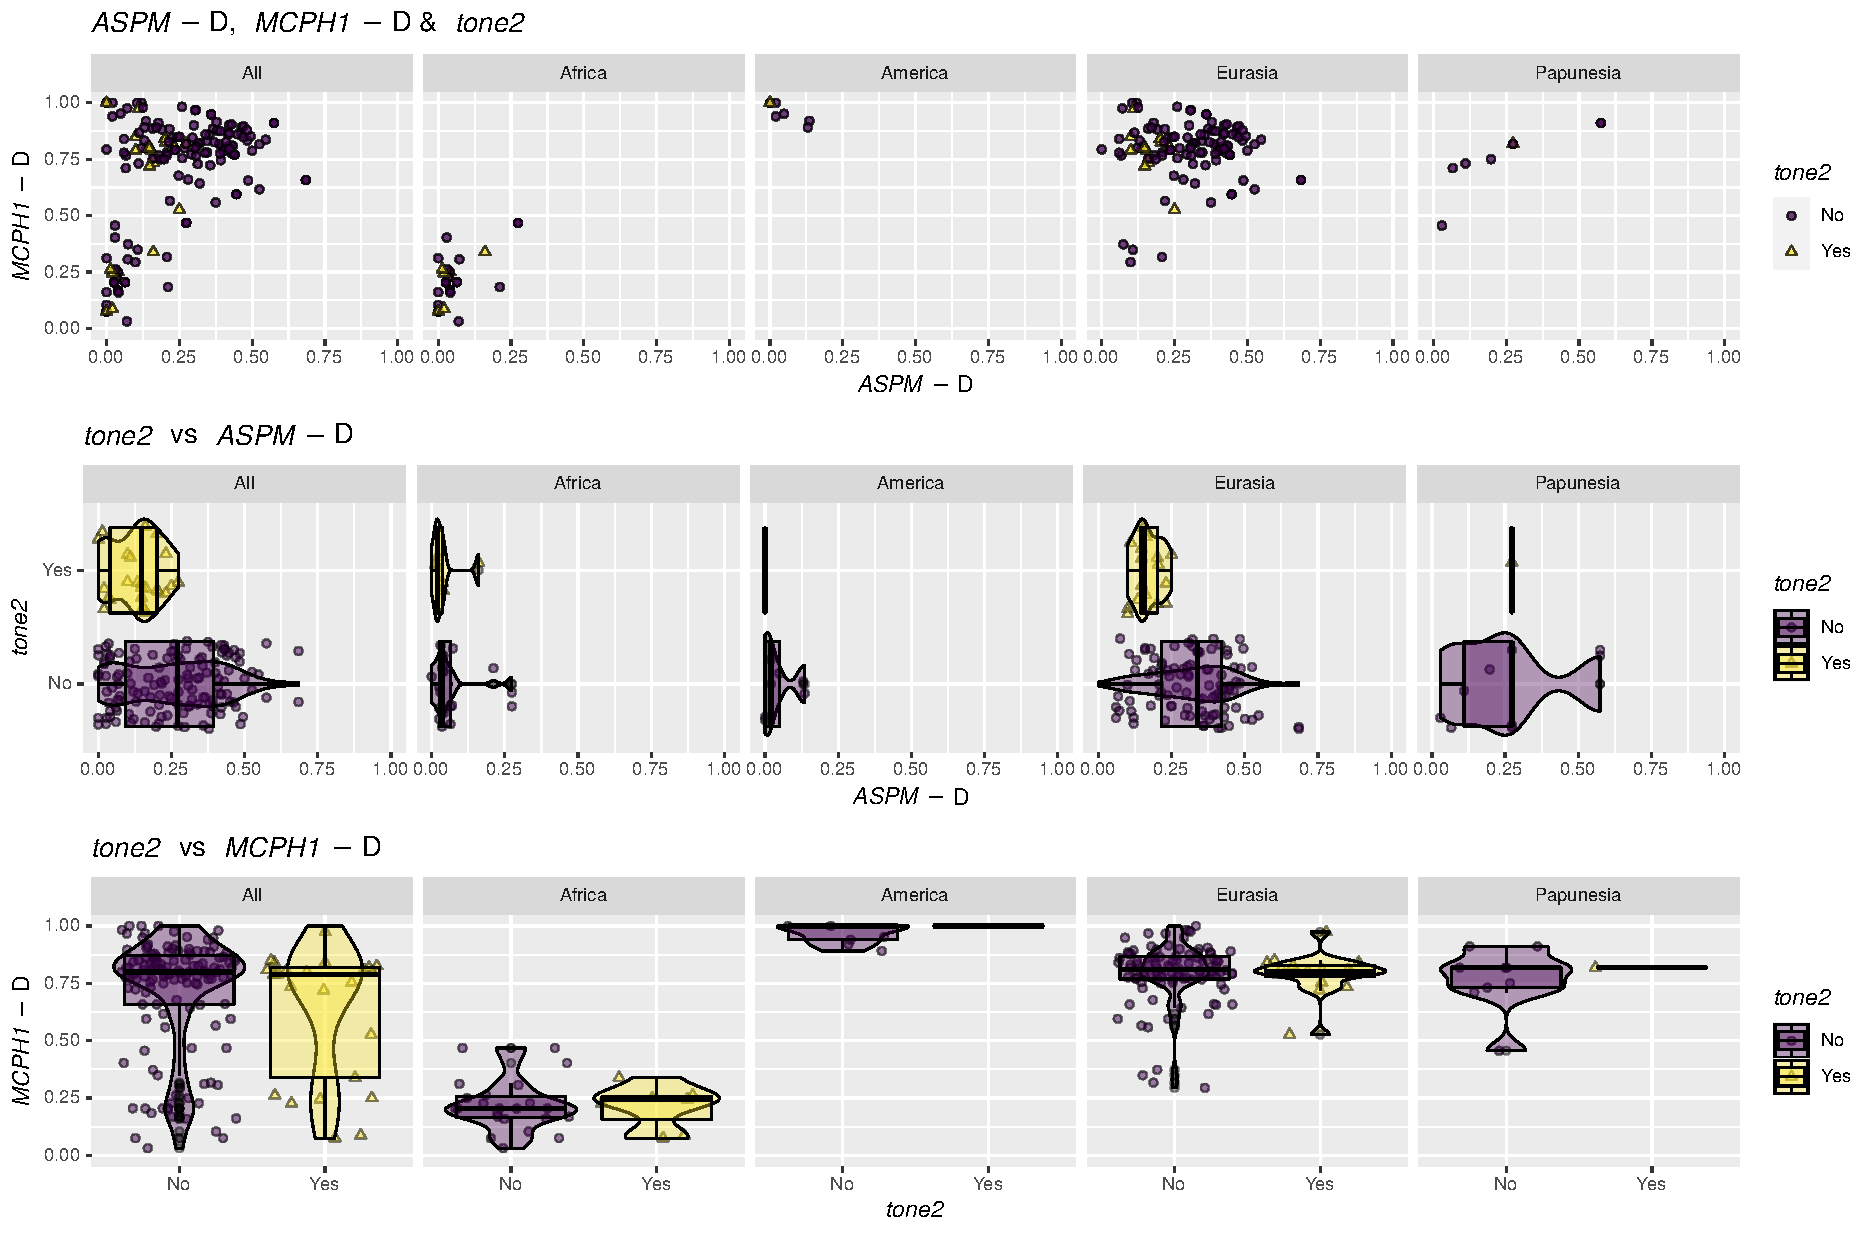
\includegraphics[width=\textwidth]{../../code/figures/tone2_alleles}
  \caption{Relationship between tone2 and the population frequency of \textit{ASPM}-D and \textit{MCPH1}-D in the whole database and separately by macroarea. Same conventions as in Figure \ref{Fig:tone1_alleles}.}
  \label{Fig:tone2_alleles}
\end{figure}


\paragraph{Regressions}

On the whole data, \textit{tone2} is almost completely clustered within families ($ICC(tone2) =94.6\%$).
The interactions do not contribute (\textit{p}(\textit{ASPM}-D:\textit{MCPH}-D) = 0.56, \textit{p}(\textit{ASPM}-D:\textit{macroarea} + \textit{MCPH}-D:\textit{macroarea}) = 0.66), that \textit{macroarea} does not predict \textit{tone2} ($p = 0.49$, $R^2 = 2.2\%$), and neither do the two ``derived'' alleles together ($p = 0.23$, $R^2 = 3.4\%$) nor individually (\textit{ASPM}-D: $\beta = -5.9 \pm 4.2$, $p = 0.14$, $R^2 = 2.4\%$; \textit{MCPH1}-D $\beta = -3.9 \pm 2.7$, $p = 0.14$, $R^2 = 2.0\%$).

However, permuting the observations shows that \textit{ASPM}-D seems to have a negative effect on \textit{tone2} (except when restricting the permutations within families while controlling for \textit{macroarea}), but \textit{MCPH1}-D seems to have a negative effect only for unrestricted permutations when not controlling for \textit{macroarea}.
Please see Figure \ref{Fig:tone2_regressions_permuted}.

\begin{figure}[h]
  \centering
  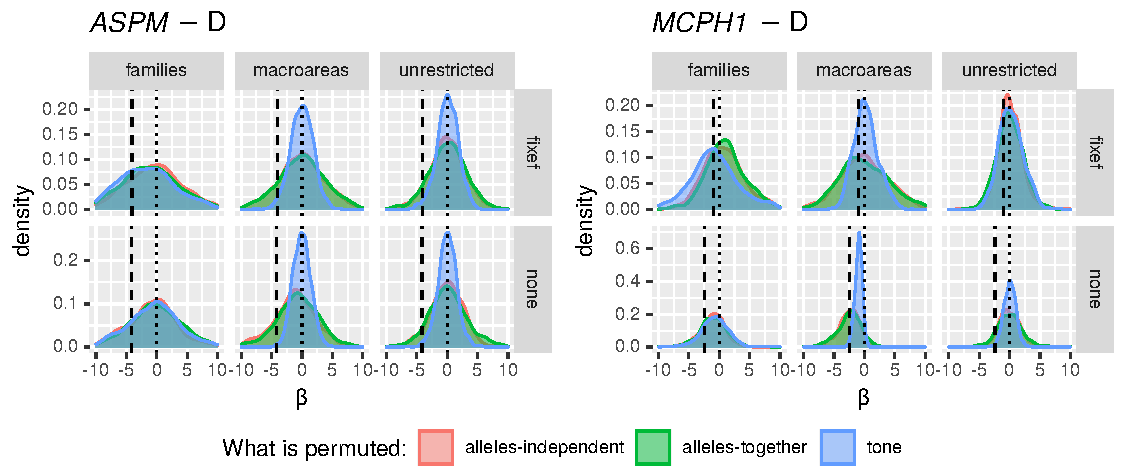
\includegraphics[width=\textwidth]{../../code/figures/tone2_regressions_permuted}
  \caption{Distribution of the permutation regressions for \textit{tone2}. Same conventions as in Figure \ref{Fig:tone1_regressions_permuted}.}
  \label{Fig:tone2_regressions_permuted}
\end{figure}

Repeated restricted sampling also shows a clear negative effect of \textit{ASPM}-D on \textit{tone2} even when controlling for \textit{macroarea} and \textit{MCPH1}-D (100\% of the $\beta$'s < 0, with a mean $\overline{\beta} = -7.6$), and arguably no effect for \textit{MCPH1}-D (37.2\% of the $\beta$'s < 0, with a mean $\overline{\beta} = 1.94$); see Figure \ref{Fig:tone2_regressions_restricted}.

\begin{figure}[h]
  \centering
  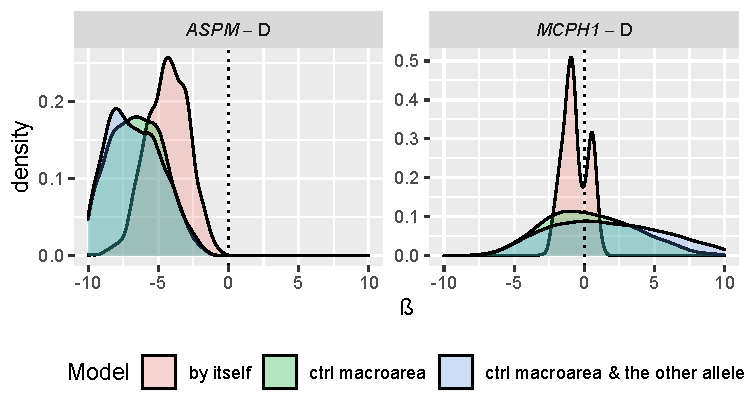
\includegraphics[width=0.6\textwidth]{../../code/figures/tone2_regressions_restricted}
  \caption{Distribution of the restricted sampling regressions for \textit{tone2}. Same conventions as in Figure \ref{Fig:tone1_regressions_restricted}.}
  \label{Fig:tone2_regressions_restricted}
\end{figure}


\paragraph{Mediation analysis}

On the full dataset, there is no significant total effect for neither of the two ``derived'' alleles (\textit{ASPM}-D: $0.13$, 95\%CI $(-0.01, 0.29)$, $p=0.064$, \textit{MCPH1}-D: $0.10$, 95\%CI $(-0.04, 0.28)$, $p=0.18$).

However, restricted sampling (Figure \ref{Fig:tone2_mediation_restricted} and Table \ref{Tab:tone2_mediation_restricted}), finds that while for both ``derived'' alleles there are positive and comparably strong total ($TE$) and direct ($ADE$) effects, only \textit{ASPM}-D shows a positive indirect effect ($ACME$), but pretty much none of these effects are individually significant.

\begin{figure}[h]
  \centering
  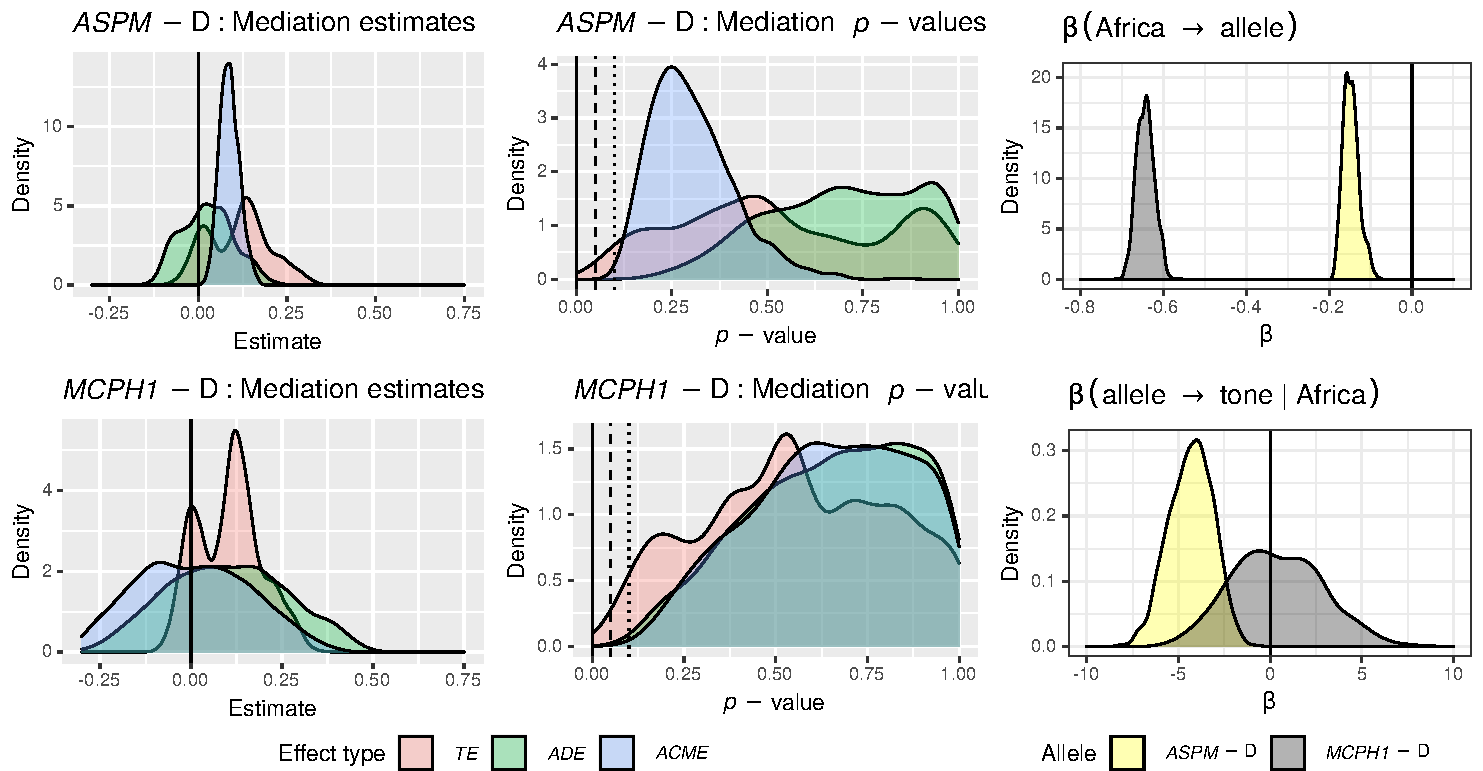
\includegraphics[width=\textwidth]{../../code/figures/tone2_mediation_restricted}
  \caption{Mediation analysis for 1,000 restricted samples for \textit{tone2}. Same conventions as in Figure \ref{Fig:tone1_mediation_restricted}. See Table \ref{Tab:tone2_mediation_restricted} for the numeric summaries.}
  \label{Fig:tone2_mediation_restricted}
\end{figure}

\begin{table}[h]
  \caption{Summaries of the mediation analysis for 1,000 restricted samples for \textit{tone2}. Same conventions as in Table \ref{Tab:tone1_mediation_restricted}.}
  \label{Tab:tone2_mediation_restricted}
  \centering
  \begin{tabular}{|l|l|r|r|l|}
    \toprule
    \textbf{Allele} & \textbf{Estimate} & \textbf{Mean} & \textbf{Median} & \textbf{Compared to 0} \\
    \midrule
    \multirow{5}{*}{\textit{ASPM}-D} & $TE$ & 0.11 & 0.13 & > 0: 91.6\%, $t = 42.2$, $p < 2.2\cdot10^{-16}$ \\
    & $ADE$ & 0.026 & 0.026 & > 0: 63.6\%, $t = 11.5$, $p < 2.2\cdot10^{-16}$ \\
    & $ACME$ & 0.088 & 0.086 & > 0: 100.0\%, $t = 100.8$, $p < 2.2\cdot10^{-16}$ \\
    & $\beta$(Africa $\rightarrow$ allele) & -0.15 &  -0.15 & < 0: 100.0\%, $t = -242.0$, $p < 2.2\cdot10^{-16}$ \\
    & $\beta$(allele $\rightarrow$ tone $\mid$ Africa) & -4.3 & -4.3 & < 0: 100.0\%, $t = -114.8$, $p < 2.2\cdot10^{-16}$ \\
    \midrule
    \multirow{5}{*}{\textit{MCPH1}-D} & $TE$ & 0.10 & 0.11 & > 0: 84.2\%, $t = 38.3$, $p < 2.2\cdot10^{-16}$ \\
    & $ADE$ & 0.099 & 0.01 & > 0: 71.1\%, $t = 19.4$, $p < 2.2\cdot10^{-16}$ \\
    & $ACME$ & 0.0056 & 0.0002 & > 0: 50.1\%, $t = 1.1$, $p = 0.13$ \\
    & $\beta$(Africa $\rightarrow$ allele) & -0.64 & -0.64 & < 0: 100.0\%, $t = -959.9$, $p < 2.2\cdot10^{-16}$ \\
    & $\beta$(allele $\rightarrow$ tone $\mid$ Africa) & 0.39 & 0.24 & < 0: 46.0\%, $t = 4.9$, $p = 1$ \\
    \bottomrule
  \end{tabular}
\end{table}


\paragraph{Path analysis}

As above, I only report here the numeric coding.
On the full dataset, the model fits the data very well ($\chi^2_{1} = 0.06$, $p = 0.81$; $CFI=1.00$, $TLI=1.02$, $NNFI=1.02$ and $RFI=1.00$).
As shown in Figure \ref{Fig:tone2_path_all}, being in Africa has no direct effect on complex tone, but has a significant negative effect on \textit{ASPM}-D which has a negative significant effect on complex tone; however, while it has a stronger significant negative effect on \textit{MCHP1}-D, this has no effect on complex tone.
The same pattern is also found by restricted sampling, except that here there is also a hint of a negative effect of \textit{MCHP1}-D on complex tone (see Figure \ref{Fig:tone2_path_restricted} and Table \ref{Tab:tone2_path_restricted}).

\begin{figure}[h]
  \centering

  \begin{tikzpicture}[node distance=4.0cm]
  \node(iv) {\textit{Africa}};
  \node(dv)[right of=iv] {\textit{tone2}};
  \node(m1)[above of=dv] {\textit{ASPM}-D};
  \node(m2)[below of=dv] {\textit{MCPH1}-D};
  \draw[->, thin, gray, dotted] (iv) -- (dv) node[midway, above] {-0.07 (0.67)};
  \draw[->, very thick, blue] (iv) -- (m1) node[midway, left] {-0.51 (0.000)};
  \draw[->, very thick, blue] (m1) -- (dv) node[midway, right] {-0.29 (0.000)};
  \draw[->, very thick, blue] (iv) -- (m2) node[midway, left] {-0.87 (0.000)};
  \draw[->, thin, gray, dotted] (m2) -- (dv) node[midway, right] {-0.03 (0.82)};
  \end{tikzpicture}

  \caption{The path model for \textit{tone2} fitted on all the data, showing the standardized path coefficients (and their \textit{p}-values in parentheses). Same conventions as in Figure \ref{Fig:tone1_path_all}. }
  \label{Fig:tone2_path_all}
\end{figure}


\begin{figure}[h]
  \centering

  \begin{tikzpicture}[node distance=4.0cm]
  \node(iv) {\textit{Africa}};
  \node(dv)[right of=iv] {\textit{tone2}};
  \node(m1)[above of=dv] {\textit{ASPM}-D};
  \node(m2)[below of=dv] {\textit{MCPH1}-D};
  \draw[->, thin, gray, dotted] (iv) -- (dv) node[midway, above] {-0.03 (0.34)};
  \draw[->, very thick, blue] (iv) -- (m1) node[midway, left] {-0.15 (0.03)};
  \draw[->, very thick, blue] (m1) -- (dv) node[midway, right] {-0.50 (0.18)};
  \draw[->, very thick, blue] (iv) -- (m2) node[midway, left] {-0.64 (0.03)};
  \draw[->, thin, gray, dotted] (m2) -- (dv) node[midway, right] {-0.06 (0.52)};
  \end{tikzpicture}

  \caption{Summary of the 1,000 path models for \textit{tone2} fitted to restricted samples, showing the medians of the standardized path coefficients (and their IQR, in parentheses). Same conventions as in Figure \ref{Fig:tone1_path_restricted}. }
  \label{Fig:tone2_path_restricted}
\end{figure}

\begin{table}[h]
  \caption{Summaries of the path analysis for 1,000 restricted samples for \textit{tone2}. Similar conventions as for Table \ref{Tab:tone1_mediation_restricted}.}
  \label{Tab:tone2_path_restricted}
  \centering
  \begin{tabular}{|l|l|r|r|l|}
    \toprule
    \textbf{Type} & \textbf{Estimate} & \textbf{Mean (SD)} & \textbf{Median (IQR)} & \textbf{Compared to 0} \\
    \midrule
    \multirow{5}{*}{Fit} & $\chi^2$ test & 99.4\% n.s. & - & - \\
    & $CFI$              & 0.99 (0.01) & 1.00 (0.01) & - \\
    & $TLI$              & 1.00 (0.08) & 1.01 (0.14) & - \\
    & $NNFI$             & 1.00 (0.08) & 1.01 (0.14) & - \\
    & $RFI$              & 0.92 (0.07) & 0.94 (0.12) & - \\
    \midrule
    \multirow{4}{*}{Path} & Africa $\rightarrow$ complex tone & -0.04 (0.25) & -0.03 (0.34) & 46.0\%  > 0 \\
    & Africa $\rightarrow$ \textit{ASPM}-D                    & -0.15 (0.02) & -0.15 (0.03) & 100.0\% < 0 \\
    & \textit{ASPM}-D  $\rightarrow$ complex tone             & -0.51 (0.13) & -0.50 (0.18) & 100.0\% < 0 \\
    & Africa $\rightarrow$ \textit{MCPH1}-D                   & -0.64 (0.02) & -0.64 (0.03) & 100.0\% < 0 \\
    & \textit{MCPH1}-D $\rightarrow$ complex tone             & -0.09 (0.37) & -0.06 (0.52) & 57.7\%  < 0 \\
    \bottomrule
  \end{tabular}
\end{table}


\paragraph{Decision trees}

The decision trees including or excluding macroarea are the same and trivial in that they uniformly predict just the majority value ``No'' and have only one split depending on the frequency of \textit{ASPM}-D ($\leq$ or > $\approx 0.27$, $p < 0.001$).


\paragraph{Random forests}

If \textit{macroarea} is included as a predictor, the random forests fit the data well (accuracy = 85.1\% $\pm$0.5\%, sensitivity = 58.0\% $\pm$14.3\%, specificity = 85.8\% $\pm$0.3\%, precision = 8.3\% $\pm$2.3\%, recall = 58.0\% $\pm$14.3\%), and the conditional random forests are even better (accuracy = 87.3\% $\pm$0.1\%, sensitivity = 99.8\% $\pm$1.7\%, specificity = 87.0\% $\pm$0.1\%, precision = 16.1\% $\pm$0.7\%, recall = 99.8\% $\pm$1.7\%), and all measures of variable importance find that \textit{ASPM}-D > \textit{MCPH1}-D > \textit{macroarea}.

Leaving macroarea out has very little effect on the fit (random forests: accuracy = 87.4\% $\pm$0.6\%, sensitivity = 64.4\% $\pm$2.8\%, specificity = 89.6\% $\pm$0.5\%, precision = 37.3\% $\pm$3.1\%, recall = 64.4\% $\pm$2.8\%; conditional random forests: accuracy = 89.1\% $\pm$0.1\%, sensitivity = 88.5\% $\pm$1.8\%, specificity = 89.1\% $\pm$0.0\%, precision = 32.0\% $\pm$0.0\%, recall = 88.5\% $\pm$1.8\%), and all three criteria agree that \textit{ASPM}-D > \textit{MCPH1}-D.


\paragraph{Conclusions}

Complex tone is much rarer than no tone and simple tone, so that the distribution of \textit{tone2} is very skewed, and the results much less clear-cut than for \textit{tone1}, but it seems that there is a negative effect of \textit{ASPM}-D on complex tone (while for \textit{MCPH1}-D the evidence is much more ambiguous).




\subsection{Tone (\textit{counts})}

There are 184 unique observations with non-missing data for tone \textit{counts}, \textit{ASPM}-D and \textit{MCPH1}-D, distributed among 121 unique Glottolg codes (languages) in 35 families (the number of languages per family ranges from 1 to 47, with mean 5.3 and median 2); see Figure \ref{Fig:tone_counts_distribution}.

\begin{figure}[h]
  \centering
  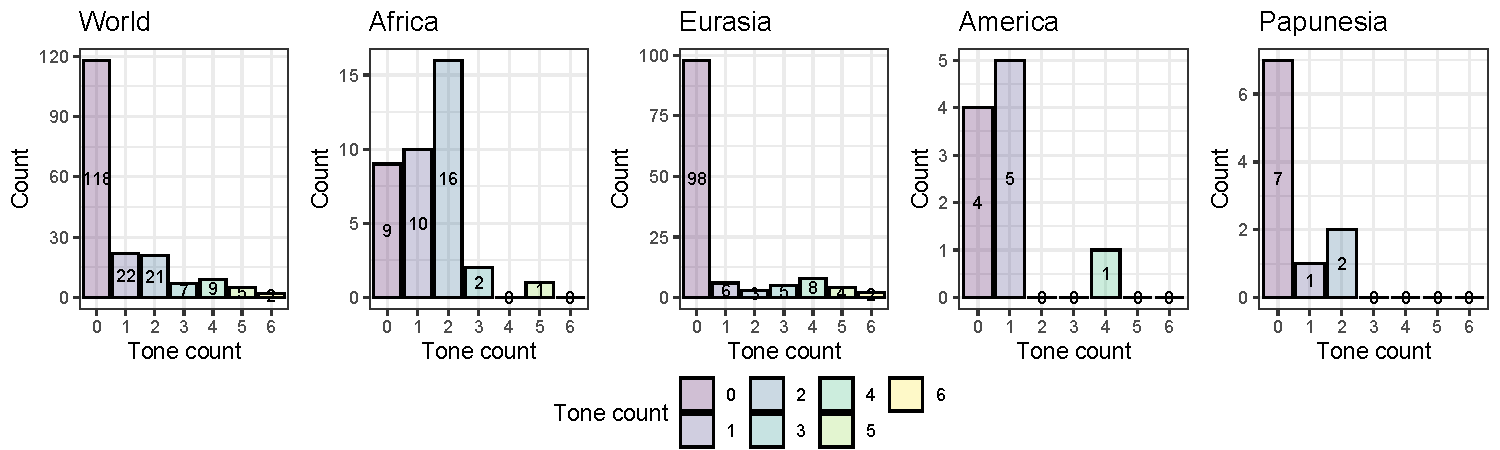
\includegraphics[width=\textwidth]{../../code/figures/tone_counts_distribution}
  \caption{Distribution of tone \textit{counts} across the full database (left-most panel) and by macroarea (the following 4 panels). Same conventions as in Figure \ref{Fig:tone1_distribution}.}
  \label{Fig:tone_counts_distribution}
\end{figure}

The relationship between the tone \textit{counts} and the population frequency of the two ``derived'' alleles is shown in Figure \ref{Fig:tone_counts_alleles}.
It can seen that, globally, languages with higher tone counts tend to be found when \textit{ASPM}-D has a low frequency, but this does not seem to be a linear relationship.

\begin{figure}[h]
  \centering
  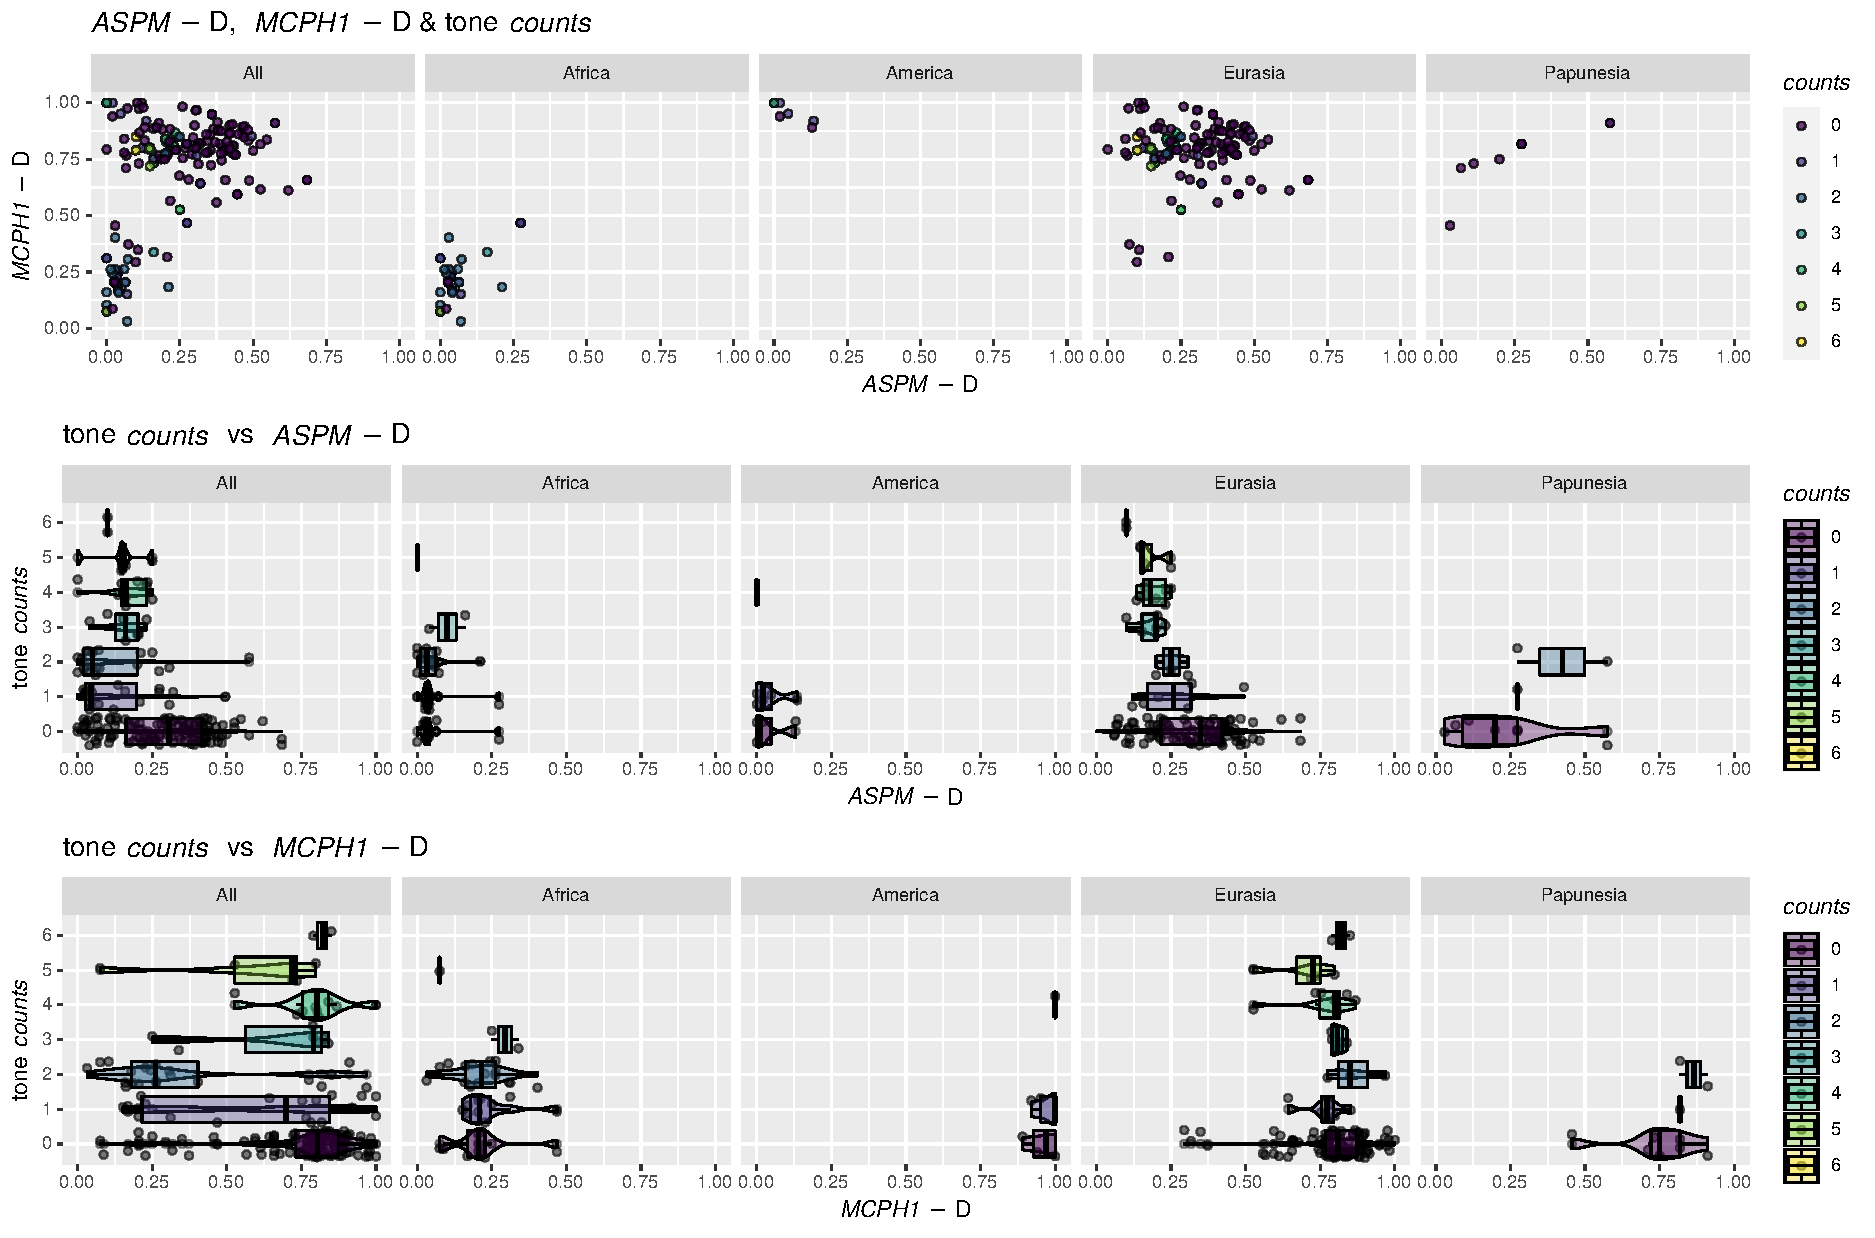
\includegraphics[width=\textwidth]{../../code/figures/tone_counts_alleles}
  \caption{Relationship between tone \textit{counts} and the population frequency of \textit{ASPM}-D and \textit{MCPH1}-D in the whole database and separately by macroarea. Same conventions as in Figure \ref{Fig:tone1_alleles}.}
  \label{Fig:tone_counts_alleles}
\end{figure}


\paragraph{Regressions}

On the whole data, the Poisson regression model is not overdispersed ($\chi^2_{182} = 112.6$, $p = 1$) and tone \textit{counts} are clustered within families ($ICC(counts) = 65.3\%$).
\textit{macroarea} predicts tone \textit{counts} ($p = 0.013$, $R^2 = 16.8\%$), \textit{ASPM}-D does not ($\beta = -2.2 \pm 1.2$, $p = 0.061$, $R^2 = 4.7\%$), while \textit{MCPH1}-D has a negative effect by itself ($\beta = -1.7 \pm 0.7$, $p = 0.016$, $R^2 = 6.5\%$) but this fully overlaps with that of \textit{macroarea}.

Permuting the observations suggests that there is a negative effect of both ``derived'' alleles when not controlling for macroarea and family; see Figure \ref{Fig:tone_counts_regressions_permuted}.

\begin{figure}[h]
  \centering
  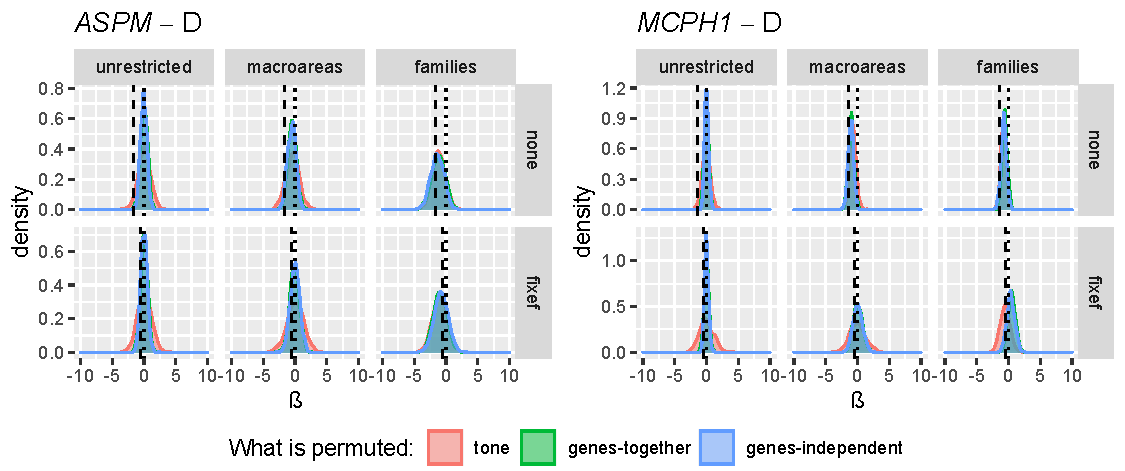
\includegraphics[width=\textwidth]{../../code/figures/tone_counts_regressions_permuted}
  \caption{Distribution of the permutation regressions for tone \textit{counts}. Same conventions as in Figure \ref{Fig:tone1_regressions_permuted}.}
  \label{Fig:tone_counts_regressions_permuted}
\end{figure}

On the other hand, restricted sampling shows a clear negative effect of \textit{ASPM}-D even when controlling for \textit{macroarea} and \textit{MCPH1}-D (96.7\% of the $\beta$'s < 0, with a mean $\overline{\beta} = -3.16$), and arguably no effect for \textit{MCPH1}-D (37.6\% of the $\beta$'s < 0, with a mean $\overline{\beta} = 1.02$); see Figure \ref{Fig:tone_counts_regressions_restricted}.

\begin{figure}[h]
  \centering
  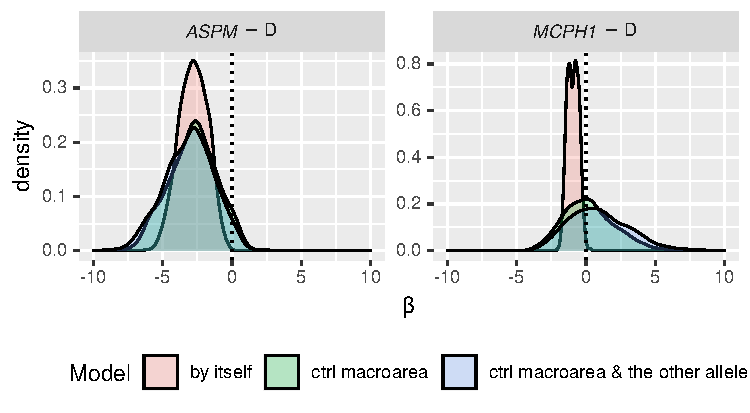
\includegraphics[width=0.6\textwidth]{../../code/figures/tone_counts_regressions_restricted}
  \caption{Distribution of the restricted sampling regressions for tone \textit{counts}. Same conventions as in Figure \ref{Fig:tone1_regressions_restricted}.}
  \label{Fig:tone_counts_regressions_restricted}
\end{figure}


\paragraph{Mediation analysis}

On the full dataset, both models find a significant positive total effect ($TE$) of macroarea on tone (\textit{ASPM}-D: $0.94$, 95\%CI $(0.42, 1.63)$, $p < 2\cdot10^{-16}$; \textit{MCPH1}-D:  $0.69$, 95\%CI $(0.31, 1.13)$, $p < 2\cdot10^{-16}$), but there is no significant direct effect ($ADE$) for neither (\textit{ASPM}-D: $-0.17$, 95\%CI $(-0.66, 0.28)$, $p = 0.47$; \textit{MCPH1}-D:  $0.43$, 95\%CI $(-0.39, 1.37)$, $p = 0.30$), and also no significant indirect effect ($ACME$) for \textit{MCPH1}-D ($0.26$, 95\%CI $(-0.55, 1.03)$, $p = 0.49$).
However, there is a significant positive $ACME$ mediated by \textit{ASPM}-D ($1.11$, 95\%CI $(0.62, 1.82)$, $p < 2\cdot10^{-16}$, mediating $\approx 100\%$ of the effect), composed of a significant negative effect of being in Africa on \textit{ASPM}-D ($-0.22 \pm0.03$, $p = 1.6\cdot10^{-15}$) and a significant negative effect of \textit{ASPM}-D on tone \textit{counts} ($-4.36 \pm0.70$, $p = 4.2\cdot10^{-10}$).

Restricted sampling (Figure \ref{Fig:tone_counts_mediation_restricted} and Table \ref{Tab:tone_counts_mediation_restricted}), finds that while for both ``derived'' alleles there are positive and comparably strong total ($TE$) and direct ($ADE$) effects, only \textit{ASPM}-D shows a positive indirect effect ($ACME$).

\begin{figure}[h]
  \centering
  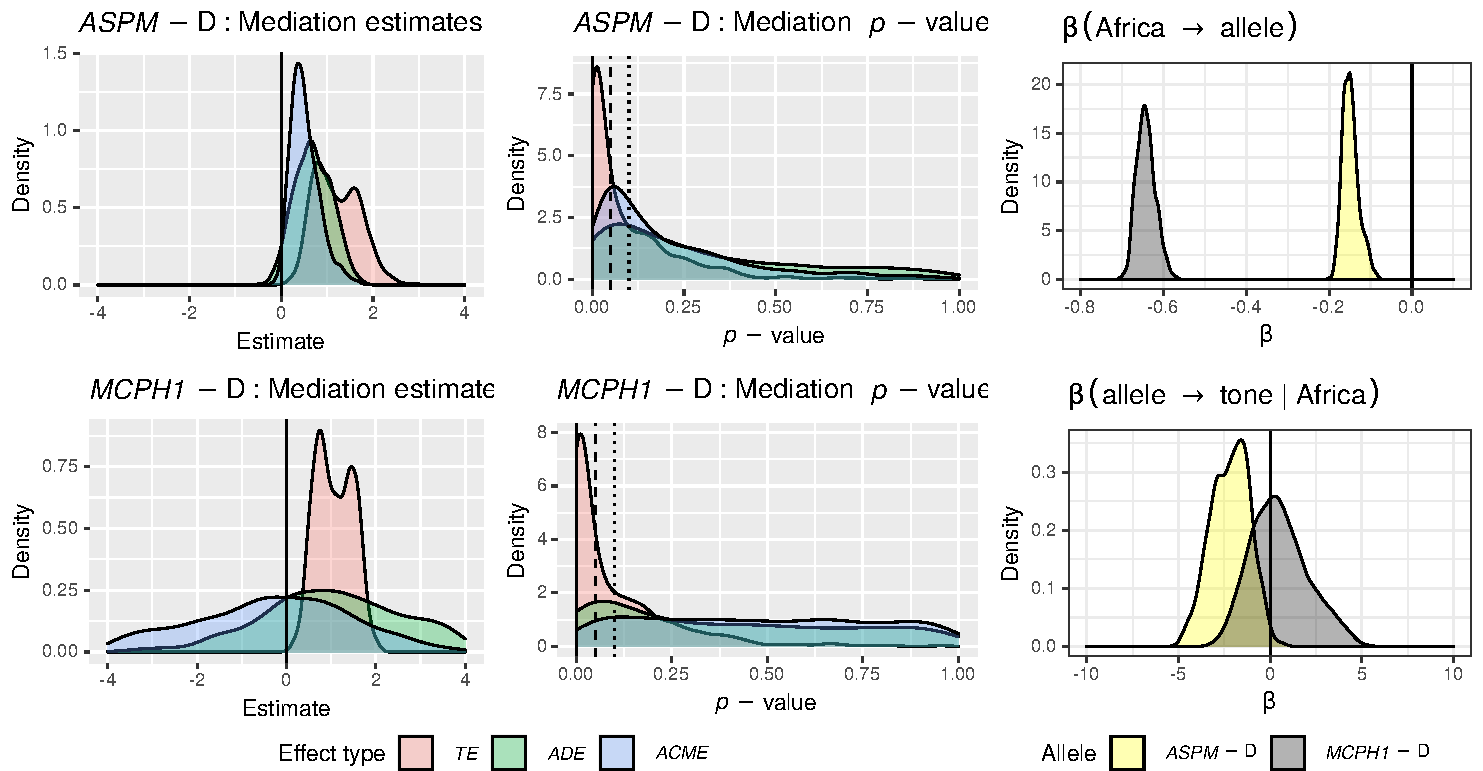
\includegraphics[width=\textwidth]{../../code/figures/tone_counts_mediation_restricted}
  \caption{Mediation analysis for 1,000 restricted samples for tone \textit{counts}. Same conventions as in Figure \ref{Fig:tone1_mediation_restricted}. See Table \ref{Tab:tone_counts_mediation_restricted} for the numeric summaries.}
  \label{Fig:tone_counts_mediation_restricted}
\end{figure}

\begin{table}[h]
  \caption{Summaries of the mediation analysis for 1,000 restricted samples for tone \textit{counts}. Same conventions as in Table \ref{Tab:tone1_mediation_restricted}.}
  \label{Tab:tone_counts_mediation_restricted}
  \centering
  \begin{tabular}{|l|l|r|r|l|}
    \toprule
    \textbf{Allele} & \textbf{Estimate} & \textbf{Mean} & \textbf{Median} & \textbf{Compared to 0} \\
    \midrule
    \multirow{5}{*}{\textit{ASPM}-D} & $TE$ & 1.2 & 1.2 & > 0: 100.0\%, $t = 77.9$, $p < 2.2\cdot10^{-16}$ \\
    & $ADE$ & 0.7 & 0.7 & > 0: 96.7\%, $t = 54.8$, $p < 2.2\cdot10^{-16}$ \\
    & $ACME$ & 0.52 & 0.46 & > 0: 99.0\%, $t = 52.0$, $p < 2.2\cdot10^{-16}$ \\
    & $\beta$(Africa $\rightarrow$ allele) & -0.15 & -0.15 & < 0: 100.0\%, $t = -237.5$, $p < 2.2\cdot10^{-16}$ \\
    & $\beta$(allele $\rightarrow$ tone $\mid$ Africa) & -2.2 & -2.1 & < 0: 99.0\%, $t = -65.9$, $p < 2.2\cdot10^{-16}$ \\
    \midrule
    \multirow{5}{*}{\textit{MCPH1}-D} & $TE$ & 1.1 & 1.0 & > 0: 100.0\%, $t = 82.1$, $p < 2.2\cdot10^{-16}$ \\
    & $ADE$ & 3.8 & 1.9 & > 0: 82.1\%, $t = 18.9$, $p < 2.2\cdot10^{-16}$ \\
    & $ACME$ & -2.7 & -0.82 & > 0: 35.2\%, $t = -13.5$, $p = 1$ \\
    & $\beta$(Africa $\rightarrow$ allele) & -0.64 & -0.64 & < 0: 100.0\%, $t = -900.5$, $p < 2.2\cdot10^{-16}$ \\
    & $\beta$(allele $\rightarrow$ tone $\mid$ Africa) & 0.50 & 0.35 & < 0: 39.8\%, $t = 10.2$, $p = 1$ \\
    \bottomrule
  \end{tabular}
\end{table}


\paragraph{Path analysis}

On the full dataset, the model fits the data very well ($\chi^2_{1} = 0.29$, $p = 0.59$; $CFI=1.00$, $TLI=1.01$, $NNFI=1.01$ and $RFI=1.00$), and, as shown in Figure \ref{Fig:tone_counts_path_all}, being in Africa has no direct effect on tone counts, but has a significant negative effect on \textit{ASPM}-D which has a negative significant effect on tone counts, but while it has a stronger significant negative effect on \textit{MCHP1}-D this has no effect on tone counts.
The same pattern is also found by restricted sampling, except that here there is also a hint of a negative effect of \textit{MCHP1}-D on complex tone (see Figure \ref{Fig:tone_counts_path_restricted} and Table \ref{Tab:tone_counts_path_restricted}).

\begin{figure}[h]
  \centering

  \begin{tikzpicture}[node distance=4.0cm]
  \node(iv) {\textit{Africa}};
  \node(dv)[right of=iv] {tone \textit{counts}};
  \node(m1)[above of=dv] {\textit{ASPM}-D};
  \node(m2)[below of=dv] {\textit{MCPH1}-D};
  \draw[->, thin, gray, dotted] (iv) -- (dv) node[midway, above] {-0.08 (0.66)};
  \draw[->, very thick, blue] (iv) -- (m1) node[midway, left] {-0.54 (0.000)};
  \draw[->, very thick, blue] (m1) -- (dv) node[midway, right] {-0.34 (0.000)};
  \draw[->, very thick, blue] (iv) -- (m2) node[midway, left] {-0.88 (0.000)};
  \draw[->, thin, gray, dotted] (m2) -- (dv) node[midway, right] {-0.09 (0.57)};
  \end{tikzpicture}

  \caption{The path model for tone \textit{counts} fitted on all the data, showing the standardized path coefficients (and their \textit{p}-values in parentheses). Same conventions as in Figure \ref{Fig:tone1_path_all}. }
  \label{Fig:tone_counts_path_all}
\end{figure}


\begin{figure}[h]
  \centering

  \begin{tikzpicture}[node distance=4.0cm]
  \node(iv) {\textit{Africa}};
  \node(dv)[right of=iv] {tone \textit{counts}};
  \node(m1)[above of=dv] {\textit{ASPM}-D};
  \node(m2)[below of=dv] {\textit{MCPH1}-D};
  \draw[->, thin, blue] (iv) -- (dv) node[midway, above] {0.83 (1.70)};
  \draw[->, very thick, blue] (iv) -- (m1) node[midway, left] {-0.15 (0.02)};
  \draw[->, very thick, blue] (m1) -- (dv) node[midway, right] {-1.80 (1.40)};
  \draw[->, very thick, blue] (iv) -- (m2) node[midway, left] {-0.64 (0.03)};
  \draw[->, thin, gray, dotted] (m2) -- (dv) node[midway, right] {0.099 (2.50)};
  \end{tikzpicture}

  \caption{Summary of the 1,000 path models for tone \textit{counts} fitted to restricted samples, showing the medians of the standardized path coefficients (and their IQR, in parentheses). Same conventions as in Figure \ref{Fig:tone1_path_restricted}. }
  \label{Fig:tone_counts_path_restricted}
\end{figure}

\begin{table}[h]
  \caption{Summaries of the path analysis for 1,000 restricted samples for tone \textit{counts}. Similar conventions as for Table \ref{Tab:tone1_mediation_restricted}.}
  \label{Tab:tone_counts_path_restricted}
  \centering
  \begin{tabular}{|l|l|r|r|l|}
    \toprule
    \textbf{Type} & \textbf{Estimate} & \textbf{Mean (SD)} & \textbf{Median (IQR)} & \textbf{Compared to 0} \\
    \midrule
    \multirow{5}{*}{Fit} & $\chi^2$ test & 98.6\% n.s. & - & - \\
    & $CFI$                              & 0.99 (0.01) & 1.00 (0.01) & - \\
    & $TLI$                              & 0.98 (0.09) & 1.00 (0.14) & - \\
    & $NNFI$                             & 0.98 (0.09) & 1.00 (0.14) & - \\
    & $RFI$                              & 0.91 (0.08) & 0.92 (0.13) & - \\
    \midrule
    \multirow{4}{*}{Path} & Africa $\rightarrow$ tone \textit{counts} &  0.83 (1.20) &  0.83 (1.70) & 75.8\%  > 0 \\
    & Africa $\rightarrow$ \textit{ASPM}-D                            & -0.15 (0.02) & -0.15 (0.02) & 100.0\% < 0 \\
    & \textit{ASPM}-D  $\rightarrow$ tone \textit{counts}             & -1.80 (0.98) & -1.80 (1.40) & 97.7\%  < 0 \\
    & Africa $\rightarrow$ \textit{MCPH1}-D                           & -0.64 (0.02) & -0.64 (0.03) & 100.0\% < 0 \\
    & \textit{MCPH1}-D $\rightarrow$ tone \textit{counts}             &  0.16 (1.80) & 0.099 (2.50) & 47.6\%  < 0 \\
    \bottomrule
  \end{tabular}
\end{table}


\paragraph{Conclusions}

The actual number of tones/tone symbols has a skewed distribution, and the results are less clear, but it seems that there is a negative effect of \textit{ASPM}-D on tone counts above and beyond the confounding effects of macroarea and family (but not for \textit{MCPH1}-D).



%------------------------------------------------

\section{Discussion and conclusions}

Using an updated dataset and methods relative to the original \citet{dediu_ladd_2007} paper, I found that the population frequencies of the two ``derived'' alleles (denoted \textit{ASPM}-D and \textit{MCPH1}-D), as well as the distribution of tone, coded as the presence/absence of any type of tone system (denoted \textit{tone1}), of complex tone systems (\textit{tone2}), or as the actual number of tones/tone symbols (tone \textit{counts}), are strongly clustered within language families and macroareas.
This is not surprising given that they are all shaped by large-scale demographic processes, with a strong vertical transmission component (inheritance), but also being influenced by horizontal processes (contact).
However, this is a very important result, as it confirms the need to properly disentangle the confounding effects of inheritance (using the language families as proxy) and contact (using the macroareas as proxy), from the potential causal effects of the two ``derived'' alleles on tone.
On the other hand, by blindly controlling for family and macroarea, we may risk ``throwing the baby with the bathwater'' in the sense that this type of causal effect is expected to act on similar timescales to the processes affecting languages and the genetic structure of populations.

Therefore, I used multiple methods of controlling for their effects, including the ``standard'' mixed-effects regression approach of modelling family as a random effect and macroarea as a fixed effect, but also by permuting the language and genetic data according to multiple types of constraints (none, within families, and within macroareas), and by repeatedly sampling only one data point from each family.
Moreover, besides the regression approach which quantifies the ``extra'' effect of the alleles on tone left after removing the effects of macroarea and family, I also used mediation and path analysis, which allow the explicit modelling of the interplay between macroarea, tone and the alleles, as well as decision trees and random forests, which quantify the capacity and relative importance of macroarea and the two alleles in predicting tone.

With these, the overall picture is one of a \emph{negative effect} of the population frequency of \textit{ASPM}-D on tone above and beyond the effects of contact (macroarea) and inheritance (family), but these effects are largely overlapping in the sense that, on the one hand, samples from the same family tend to be very similar to each other genetically and linguistically, while, on the other, being a sample from Africa or from outside Africa has a major effect on \textit{ASPM}-D and (much less so) on tone.
This ``extra'' negative effect of \textit{ASPM}-D on tone means that languages spoken by populations with a high frequency of \textit{ASPM}-D tend, overall, to not use tone, and, if they do, to have a simpler tone system than expected.
It is interesting to note that the distribution of tone languages is clearly skewed relative to the high frequencies of \textit{ASPM}-D, and it is interesting to note that there is a qualitative change around 25\% from \textit{Abau} (glottocode \texttt{abau1245}, Sepik; simple system; 57.5\% \textit{ASPM}-D), \textit{Swedish} (\texttt{swed1254}, Indo-European; simple ``pitch accent''; two samples with 49.5\% and 43.8\%), \textit{Western Balochi} (\texttt{west2368}, Indo-European; simple; 32.0\%), \textit{Eastern Panjabi} (\texttt{panj1256}, Indo-European; simple system; 30.7\%), \textit{Burushaski} (\texttt{buru1296}, Burushaski; probably not?; 28.0\%), \textit{Awngi} (\texttt{awng1244}, Afro-Asiatic; simple; 27.4\%), and a set of 7 Austronesian languages (\texttt{cemu1238}, \texttt{fwai1237}, \texttt{kara1486}, \texttt{labu1248}, \texttt{kuma1276}, \texttt{xara1244} and \texttt{yabe1254}) ambiguously matching the ``Micronesians'' (\textit{ALFRED} \texttt{SA004382R}) genetic sample with 27.3\% \textit{ASPM}-D with simple tone systems, to \textit{L\"{u}} and \textit{Tai N\"{u}a} (\texttt{luuu1242} and \texttt{tain1252}, Tai-Kadai; complex to systems; 25.0\%), \textit{Sichuan Yi} (\texttt{sich1238}, Sino-Tibetan; simple; 25.0\%), \textit{She} (\texttt{shee1238}, Hmong-Mien; complex; 23.4\%) and \textit{Mandarin Chinese} and \textit{Yue Chinese} (\texttt{mand1415} and \texttt{yuec1235}, Sino-Tibetan; complex; 23.1\%).
At the other extreme, a low frequency of \textit{ASPM}-D clearly does not require the presence of tone.

However, while \textit{MCPH1}-D apparently also has a negative effect on tone on its own, this effect seems to be fully driven by its very skewed distribution within versus outside Africa.

Thus, the more (and, in some cases, more refined) data that became available since 2007 concerning both the population frequency of the two ``derived'' alleles (either directly, or inferred through proxies in high linkage disequilibrium) and tone, and the newer methods that became popular since, support a \emph{weak negative effect of \textit{ASPM}-D but not of \textit{MCPH1}-D} after removing the effects of contact (macroareas) and inheritance (language families).

Interestingly, while the original data and analyses in \citet{dediu_ladd_2007} did not find anything that would suggest a qualitative difference between \textit{ASPM}-D and \textit{MCPH1}-D in how they affect tone, the results reported here do, with the effect of \textit{MCPH1}-D apparently fully confounded by its skewed distribution inside versus outside Africa.
This is consonant with the experimental findings of \citet{wong_plosone_2012} and \citet{wong_sciadv_2020}, which supported a (negative) effect of \textit{ASPM}-D on tone perception/processing, but failed to find any effect of \textit{MCPH1}-D.

Methodologically, the mixed-effects regressions with family as random effect and macroarea as fixed effect were the most conservative, failing to find an effect of the ``derived'' alleles on tone.
Randomising the data allows a better insight into the influence of the confounds and the differences between \textit{ASPM}-D and \textit{MCPH1}-D.
Repeatedly sampling only one language per family (``restricted sampling'') coupled with regression modelling and controlling for macroarea is better at disentangling the negative effect of \textit{ASPM}-D on tone.
The mediation and path analyses, especially when coupled with restricted sampling (controlling thus for inheritance), clearly show that the main confound is being or not an African sample/language and that this shapes both the distribution of the two ``derived'' alleles and of tone, but also that while it fully explains the apparent effect of \textit{MCPH1}-D it only partly accounts for that of \textit{ASPM}-D on tone.
The decision trees and random forests must be seen only as providing some supporting evidence that indeed \textit{ASPM}-D is an important predictor of tone besides macroarea.

Finally, I think the relationship between tone and \textit{ASPM}-D, but probably not with \textit{MCPH1}-D, may be one of the most beautiful illustrations of the joys and perils of \emph{exploratory analyses}: rather than being fishy ``fishing expeditions'' that no decent scientist should embark on, they are essential tools for the advancement of science, generating the hypotheses that other methods are designed to test.
However, there are costs and benefits to everything, and the relationship between the two should be an open decision, adapted to each field and question: too high an aversion for potential false positives and there goes the effect of \textit{ASPM}-D on tone; too liberal, and \textit{MCPH1}-D is allowed to ``sneak'' into the rather select club of genes that do something to tone.
Luckily, due to the nature of linguistics, temporarily accepting \textit{MCPH1}-D in the ``causal'' club (very probably a false positive of \citealp{dediu_ladd_2007}) together with \textit{ASPM}-D (seemingly a true positive of that study) did not kill any patients, blow up any multi-billion euro infrastructure, contribute to climate inaction, nor radicalise any vulnerable persons.
On the other hand, missing the effects of \textit{ASPM}-D on tone would have arguably delayed the reintegration of language in its wider environment and the current ``renaissance'' of extra-linguistic explanations for language evolution, change and diversity \citep{blasi_human_2019,dediu_language_2017,everett_language_2016,dediu_glossa_2019,lupyan_why_2016}, which is part of a larger paradigm shift within the language sciences that matters beyond linguistics.

To be clear, I am as far as imaginable from arguing for the unbridled dredging of databases for correlations between acacia trees and car accidents \citep{ladd_correlational_2015,roberts_traffic_2013}!
Exploratory studies are complex endeavours that must use high-quality data, an up-to-date methodological toolkit, and a proper understanding of the substantive issues at hand, in order to weed out as many of the false positives and spurious correlations as possible.
We must keep in mind that there’s no such thing as a free lunch: while missing connections (false negatives) comes at the expense of failing to push the boundaries of science, being too accepting and/or methodologically weak results in too many false positives which, as dramatically shown by the ``replicability crises'' in medicine \citep{ioannidis_why_2005} and social sciences – as only the most visible cases – has tremendous negative consequences for science in terms of wasted resources, loss of trust, and factually wrong views becoming widespread among the public at large with real-life consequences \citep{bregman_humankind_2020}.






%------------------------------------------------

\section*{Acknowledgements}

Special thanks D. Robert Ladd and Patrick Wong.
I also wish to thank \textit{Huma-num} (\url{https://www.huma-num.fr}) for the use of their computing infrastructure for parts of this project.


%------------------------------------------------

\section*{Funding}

I was funded by an IDEXLYON (16-IDEX-0005) Fellowship grant (2018-2021), and indirectly by the LabEx ASLAN (ANR-10-LABX-0081) of the University of Lyon within the program Investissements d’Avenir (ANR-11-IDEX-0007) of the French National Research Agency (ANR).


%------------------------------------------------

\section*{Author contributions}

I am the sole author of this paper.


%------------------------------------------------

\section*{Ethics}

Not applicable.


%------------------------------------------------

\section*{Conflict of interests}

I declare no conflict of interest.


%----------------------------------------------------------------------------------------
%	REFERENCE LIST
%----------------------------------------------------------------------------------------

\bibliography{references}
%----------------------------------------------------------------------------------------


%------------------------------------------------

\onecolumn
\section{Supplementary materials}

All the data and \texttt{R} and \texttt{Rmarkdown} code need to reproduce these results, as well as the full results (as a self-contained \texttt{HTML} document) are freely available in the GitHub repository \url{https://github.com/ddediu/tone-genes-update}.
All external file paths are relative to the root of this repository (e.g., \verb|./data/genetics/code/00_preprocesses_genetics.R|).


\subsection{Population matching} \label{SM:pop_match}

The meta-information used for matching samples and (meta)populations is contained in the \texttt{TAB}-separated file \verb|./data/genetics/input/populations.tsv|, and is used in the pre-processing of the genetic data by the \texttt{R} script \verb|./data/genetics/code/00_preprocesses_genetics.R|.


\subsection{Agreement between sources for tone} \label{SM:tone_agreeemnt_sources}

A summary is given in Figure \ref{Fig:tone_agreement_sources}, but for full details please see the \texttt{HTML} analysis report \verb|./data/genetics/code/tone-genes.html|.

\begin{figure}[h]
  \centering
  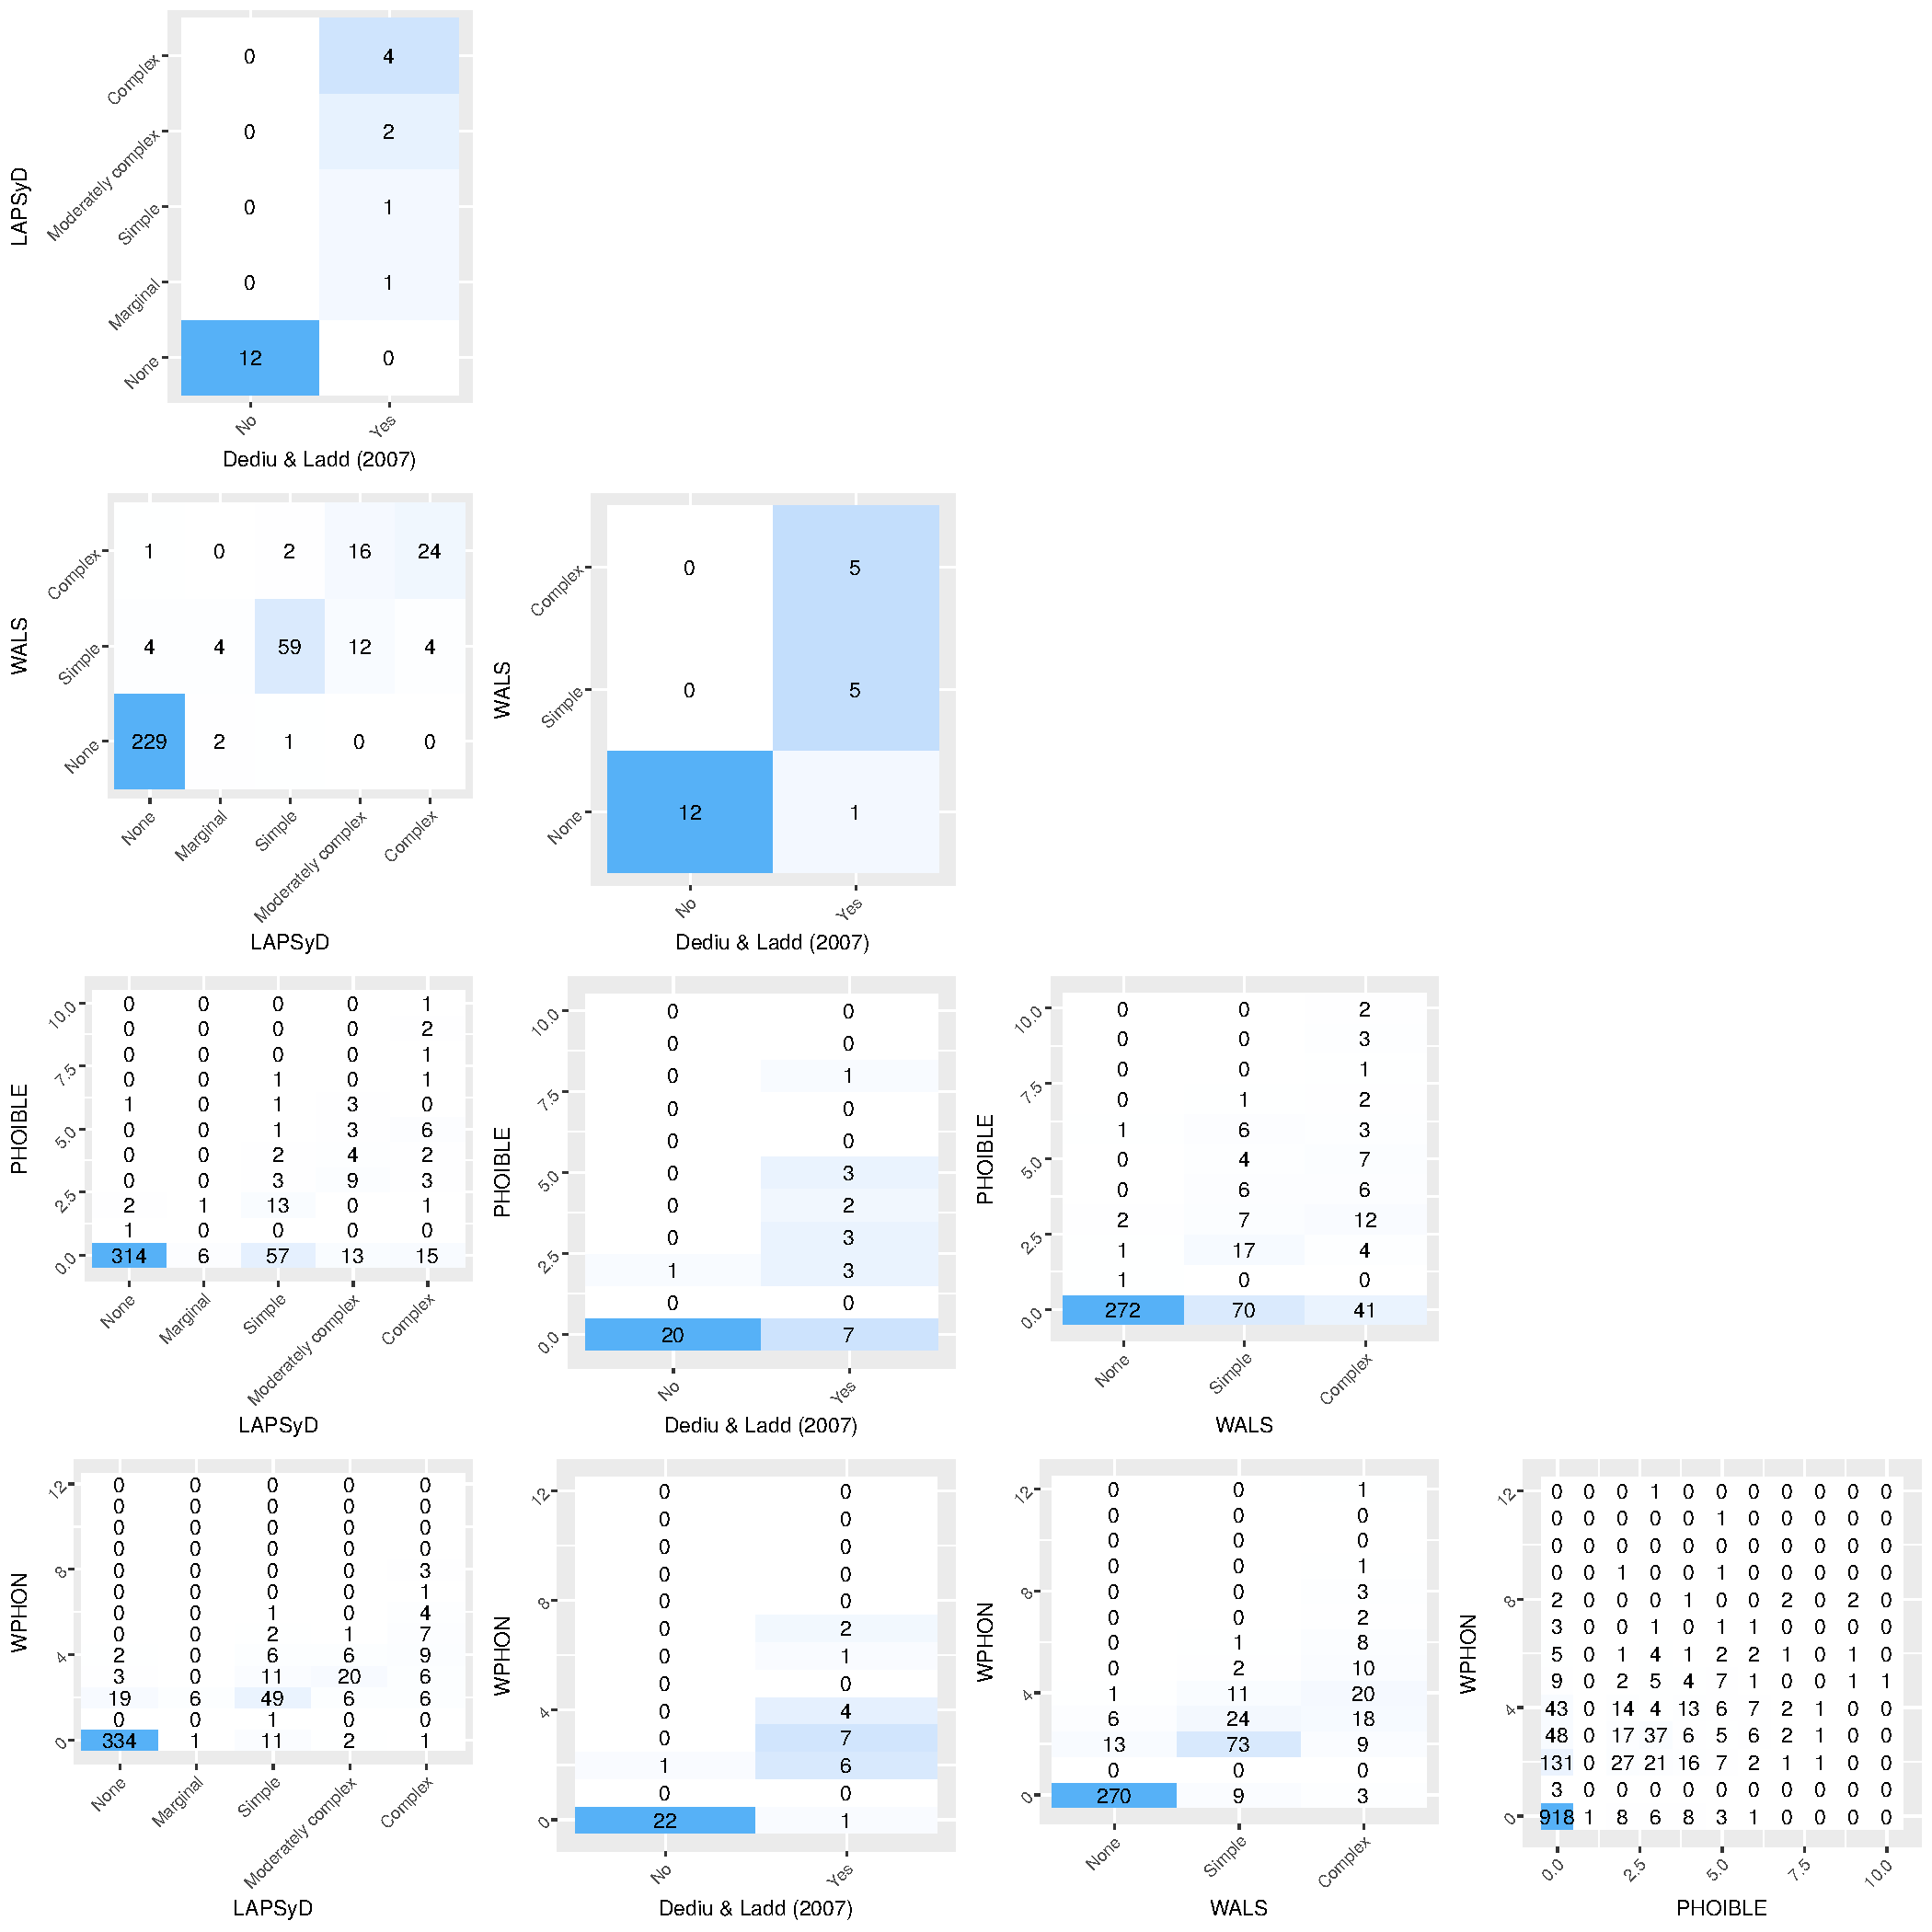
\includegraphics[width=\textwidth]{../../code/figures/tone_agreement_sources}
  \caption{The agreement between the 5 sources for tone. Each panel shows a pair of sources (e.g., the top-left panel shows \textit{LAPSyD} on the vertical axis and \textit{DL2007} on the horizontal axis); please note that the pairs are symmetric, so that the \textit{DL2007} vs \textit{LAPSyD} panel is not shown; likewise, the identity panels (e.g., \textit{LAPSyD} vs \textit{LAPSyD}) on the diagonal are also not shown. Each panel shows the number of languages with each possible combination of values from the two sources (e.g., for ``None'' vs ``No'', there are 12 languages, but there's no language for ``None'' vs ``Yes''). The shade of blue varies between white (the lowest count) to light blue (highest count). A high agreement between two sources results in little discrepancy between corresponding values (e.g., all ``None'' in \textit{LAPSyD} map to ``No'' in \textit{DL2007} and vice-versa, while ``Marginal'', ``Simple'', ``Moderately complex'' and ``Complex'' map to ``Yes'').}
  \label{Fig:tone_agreement_sources}
\end{figure}


\subsection{Agreement classification of tone vs the sources} \label{SM:tone_agreeemnt_with_sources}

A summary is given in Figures \ref{Fig:tone_agreement_with_sources_binary},  \ref{Fig:tone_agreement_with_sources_3way}, and  \ref{Fig:tone_agreement_with_sources_counts}, but for full details please see the \texttt{HTML} analysis report \verb|./data/genetics/code/tone-genes.html|.

\begin{figure}[h]
  \centering
  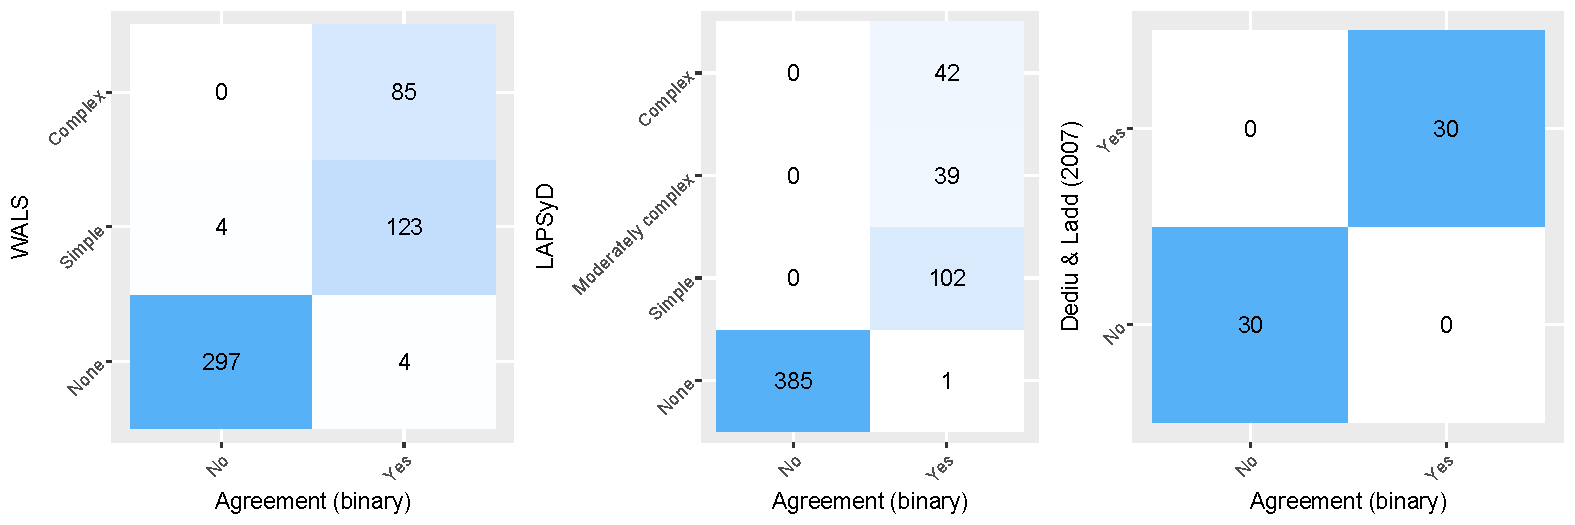
\includegraphics[width=\textwidth]{../../code/figures/tone_agreement_with_sources_binary}
  \caption{The agreement binary classification of tone versus the original sources \textit{WALS}, \textit{LAPSyD} and \textit{DL2007}. The same conventions as for Figure \ref{Fig:tone_agreement_sources}).}
  \label{Fig:tone_agreement_with_sources_binary}
\end{figure}

\begin{figure}[h]
  \centering
  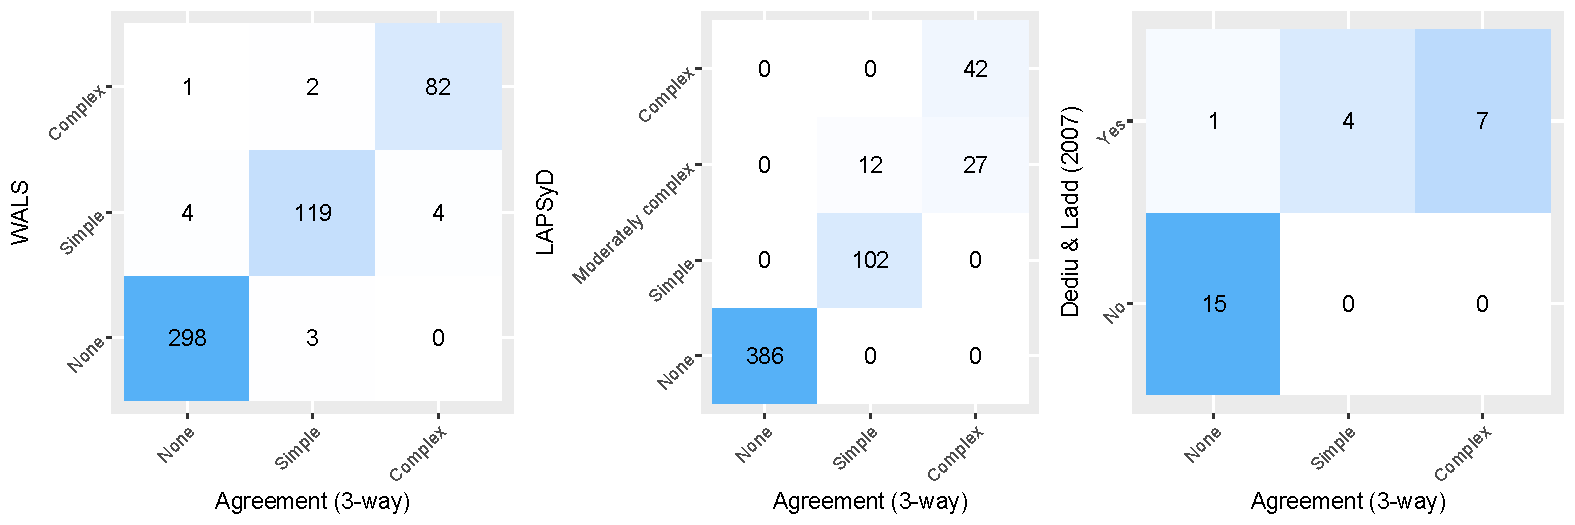
\includegraphics[width=\textwidth]{../../code/figures/tone_agreement_with_sources_3way}
  \caption{The agreement 3-way classification of tone versus the original sources \textit{WALS}, \textit{LAPSyD} and \textit{DL2007}. The same conventions as for Figure \ref{Fig:tone_agreement_sources}).}
  \label{Fig:tone_agreement_with_sources_3way}
\end{figure}

\begin{figure}[h]
  \centering
  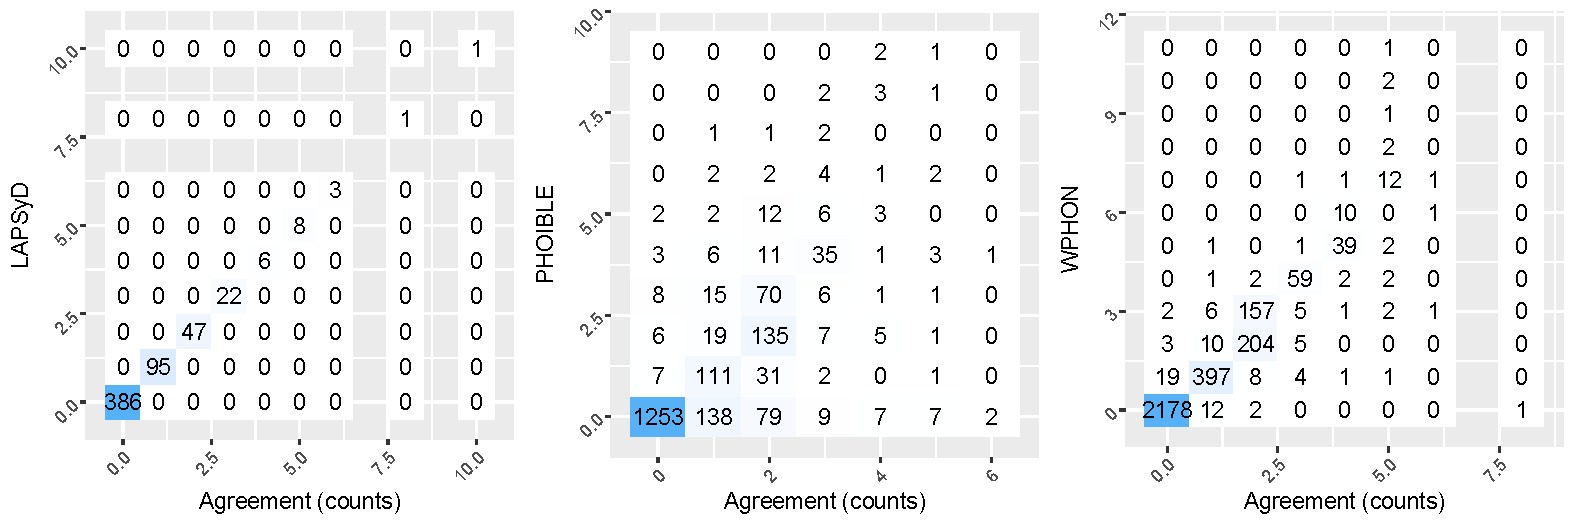
\includegraphics[width=\textwidth]{../../code/figures/tone_agreement_with_sources_counts}
  \caption{The agreement for tone counts versus the original sources \textit{LAPSyD}, \textit{PHOIBLE} and \textit{WPHON}. The same conventions as for Figure \ref{Fig:tone_agreement_sources}).}
  \label{Fig:tone_agreement_with_sources_counts}
\end{figure}



\end{document}
